\documentclass[12pt]{article} % use larger type; default would be 10pt

%packages
\usepackage{epsfig}
\usepackage{amsmath}
\usepackage{authblk}
\usepackage{setspace}
\usepackage[mathlines]{lineno}
\usepackage[margin=1in]{geometry}
\usepackage{float}
\usepackage{gensymb}
\usepackage{lscape}
\usepackage{braket}
%\usepackage{hyperref}
%\usepackage[options]{nohyperref}
\usepackage{url}
\usepackage{afterpage}
\usepackage{fancyhdr}
\usepackage[defaultlines=3,all]{nowidow}
\usepackage[absolute]{textpos}
\usepackage{tocloft}

\usepackage{times}

\usepackage{multirow}
\usepackage{titlesec}
\setcounter{secnumdepth}{2}
\titleformat{\paragraph}
{\normalfont\normalsize\bfseries}{\theparagraph}{1em}{}
% \titlespacing*{\paragraph}
% {0pt}{3.25ex plus 1ex minus .2ex}{1.5ex plus .2ex}
\titlespacing*{\paragraph}
{0pt}{0in}{1.5ex plus .2ex}

\usepackage{cancel}
\usepackage{booktabs}

%\titleformat{\section}{\singlespacing\normalfont\Large\bfseries}{\thesection}{0.5em}{\centering\MakeUppercase}[\vspace{1ex}]
\titlespacing\section{0in}{-0.3in}{0.4in}
\titleformat{\section}{\singlespacing\Large\bfseries}{\thesection}{0.5em}{\centering\MakeUppercase}
%\titlespacing*{\section}{0pt}{3.25ex plus 1ex minus .2ex}{1.5ex plus .2ex}
%\titlespacing\subsection{0in}{0in}{0in}
\titleformat{\subsection}[block]{\singlespacing\large\bfseries}{\thesubsection}{0.5em}{}
\titleformat{\subsubsection}[block]{\singlespacing\bfseries}{}{0em}{}

\setlength{\cftsubsecnumwidth}{3em}
\setlength{\cftsubsubsecnumwidth}{3em}

\renewcommand\cftdotsep{5}

\renewcommand\cfttoctitlefont{\normalfont\MakeUppercase}
\renewcommand{\contentsname}{\hfill Table of Contents\hfill}
\renewcommand\cftaftertoctitle{\hfill}
\setlength\cftbeforetoctitleskip{0.5in}
\setlength\cftaftertoctitleskip{0.4in}

\renewcommand\cftsecfont{\normalfont}
\renewcommand{\cftsecleader}{\cftdotfill{\cftsecdotsep}}
\renewcommand\cftsecdotsep{\cftdotsep}
\renewcommand\cftsecpagefont{\normalfont}
\setlength\cftbeforesecskip{0in}

% \makeatletter
% \renewcommand\tableofcontents{%
%     \@starttoc{toc}%
% }
% \makeatother

\begin{document}

\doublespacing

\thispagestyle{empty}
\begin{center}
DISSERTATION\\

\bigskip
\bigskip
\bigskip
\bigskip
\bigskip

MEASUREMENT OF $\nu_\mu$ INDUCED CHARGED CURRENT\\ 
INCLUSIVE CROSS SECTION ON WATER USING THE\\
NEAR DETECTOR OF THE T2K EXPERIMENT\\

\bigskip
\bigskip
\bigskip
\bigskip
\bigskip

Submitted by\\
Rajarshi Das\\
Department of Physics\\

\bigskip
\bigskip
\bigskip
\bigskip
\bigskip

In partial fulfillment of the requirements\\
For the Degree of Doctor of Philosophy\\
Colorado State University\\
Fort Collins, Colorado\\
Spring 2016
\end{center}

\bigskip
\bigskip
\bigskip
\bigskip

\singlespacing
\noindent Doctoral Committee:\\

\indent Advisor: Walter Toki\\
%\indent Co-Advisor: Robert Wilson\\

\indent Robert Wilson\\
\indent Bruce Berger\\
\indent Carmen Menon\\


\newpage

\thispagestyle{empty}
\topskip0pt
\vspace*{\fill}
\doublespacing
\begin{center}
Copyright by Rajarshi Das 2016\\
All Rights Reserved
\end{center}
\vspace*{\fill}

\newpage
\pagenumbering{roman}

\setstretch{2}

\setcounter{page}{2}
\addcontentsline{toc}{section}{Abstract}
\begin{center}
ABSTRACT\\
\bigskip
MEASUREMENT OF $\nu_\mu$ INDUCED CHARGED CURRENT INCLUSIVE CROSS SECTION ON WATER USING THE NEAR DETECTOR OF THE T2K EXPERIMENT\\
\end{center}
\medskip
\-\ \indent The Tokai to Kamioka (T2K) Experiment is a long-baseline neutrino oscillation experiment located in Japan with the primary goal to measure precisely multiple neutrino flavor oscillation parameters. An off-axis muon neutrino beam peaking at 600 MeV is generated at the JPARC facility and directed towards the 50 kiloton Super-Kamiokande (SK) water Cherenkov detector located 295 km away. Measurements from a Near Detector that is 280 m downstream of the neutrino beam target are used to constrain uncertainties in the beam flux prediction and neutrino interaction rates. We present a selection of inclusive charged current neutrino interactions on water. We used several sub-detectors in the ND280 complex, including a Pi-Zero detector (P0D) that has alternating planes of plastic scintillator and water bag layers, a time projection chamber (TPC) and fine-grained detector (FGD) to detect and reconstruct muons from neutrino charged current events. We use a statistical subtraction method with the water-in and water-out inclusive selection to extract a flux-averaged, $\nu_\mu$ induced, charged current inclusive cross section. We also outline the evaluation of systematic uncertainties. We find an absolute cross section of $\left<\sigma\right>_\Phi = (6.37 \pm 0.157 (stat.) ^{-1.060}_{+0.910} (sys.))\times 10^{-39} \frac{cm^2}{H_2O\:nucelon}$. This is the first $\nu_\mu$ charged current inclusive cross section measurement on water. 

\newpage
\addcontentsline{toc}{section}{Acknowledgments}
\begin{center}
ACKNOWLEDGMENTS
\end{center}
\medskip
\-\ \indent This thesis would not be possible without three groups of people. First, I would like to thank my advisor Walter Toki. Without his guidance and superhuman patience, graduate school would have been an impossible feat. Second, I want to thank all of my friends, new and old, for the gifts of love and laughter through the years. Finally, I want to thank my family: my uncle, my mother and my father. They provided support in too many ways to count, even when I myself didn't know I needed it. I don't think my father knew when he first showed me a magnet that he had just set my young feet on a journey that will last the rest of my life.
\pagebreak






\newpage

\setcounter{secnumdepth}{2}
\setcounter{tocdepth}{2}
% \begin{center}
% TABLE OF CONTENTS
% \end{center}
\tableofcontents

\clearpage

\pagenumbering{arabic}
\setcounter{page}{1}

\setstretch{2}
\section{Introduction}
\label{sec:Introduction}

Almost 85 years ago, Wolfgang Pauli proposed to the physics community the existence of a neutral, weakly interacting particle that would solve the baffling problem of the continuous $\beta$ decay energy spectrum. In the many decades that have passed, not only has the $\beta$ spectrum puzzle been solved, but the story of this little particle, dubbed the ``neutrino", has grown into an entire science. The study of neutrino properties and their interactions with matter have consumed many millions of man-hours and motivated the construction of enormous technological structures all over the world. 

In 1960, Davis and Bahcall found a deficit in the number of expected neutrinos from the sun; a problem with the rather surprising solution that particular flavors of neutrinos could somehow \emph{disappear} and \emph{reappear} over time and distance. Evidence for this phenomenon, called neutrino oscillation, was later discovered by Super Kamiokande and published in the most cited particle physics paper of all time. The Solar Neutrino Observatory (SNO) later confirmed that neutrino mixing in combination with the matter effect solved the solar neutrino problem. Neutrinos have also proved instrumental in probing the structure of a nucleon. Yet many mysteries remain unraveled. Neutrinos have mass, but how much mass? Are they Dirac or Majorana particles? Can neutrino oscillation violate charge-parity conservation and even further the understanding of the matter-antimatter asymmetry of our universe? These questions and more mean that the study of neutrinos will remain a fascinating and growing field.

The T2K experiment is one of a few long-baseline neutrino experiments designed to measure the parameters that govern neutrino oscillation. The far detector of T2K is the same Super Kamiokande responsible for the discovery of neutrino mixing. Super Kamiokande is a water Cherenkov detector, so measurement of oscillation parameters requires an accurate knowledge of the neutrino interaction rate on water. Also, neutrino nucleon interactions are the only way to measure the axial form factors of the nucleon current. With such motivations, the need for a neutrino cross section on water is clear.

In this thesis, we present a measurement of the $\nu_\mu$ induced charged current inclusive cross section on water using the Pi-Zero detector and the Tracker of the off-axis near detector complex in the T2K experiment. In a $\nu_\mu$ CC inclusive interaction, we expect a daughter muon to be produced. Using the uniquely designed water target of the P0D as a neutrino interaction target, and the TPC for its muon reconstruction, we select the daughter muon in the charged current event. The neutrino event rate in the P0D while it is drained of water is statistically subtracted from the neutrino event rate in the P0D while it is filled with water.

In Chapter \ref{sec:Theory}, we first discuss the formalism describing neutrino oscillation and then summarize the calculation of the three main neutrino-nucleon scattering processes in the 1~GeV regime: quasi-elastic, resonance production and deep inelastic scattering. Then, in Section \ref{sec:detectordescription}, we provide a description of the T2K experiment, focusing on the near detector complex where the cross section measurement is carried out. Section \ref{sec:FluxDetermination} discusses how the muon neutrino flux at the near detector is determined and Section \ref{sec:evsim} describes the neutrino interaction simulation and how T2K uses external data to constrain cross section parameters. Section \ref{sec:Reconstruction} explains the event reconstruction process. Then Section \ref{sec:fidmassvol} describes how the mass of water in the analysis fiducial volume is measured. Section \ref{sec:selection} describes the selection process used to identify candidate muon neutrino events and shows the resulting distributions. Section \ref{sec:xsec} uses the selected event rates and develops the statistical subtraction method used to extract the water-only cross section from two separate samples. Sections \ref{sec:fluxxsecsyst}, \ref{sec:detsys} and \ref{sec:detsysprop} explain how flux, cross section parameter and detector systematic uncertainties are measured and propagated into the water cross section measurement. Finally, Section \ref{sec:results} discusses the final measurement of the $\nu_\mu$ charged-current inclusive cross section on water and compares it to available global data. 

As with all modern neutrino experiments, T2K is a large collaboration. A collection of theorists, experimentalists, engineers and graduate students are intellectually responsible for the complete set of analyses performed using T2K apparatus. A lot of information in this thesis is extracted from publications, presentations, notes and technical documents written by these people. It is therefore important to highlight my personal intellectual contributions to this thesis. In close collaboration with small analysis groups at Colorado State University, Fort Collins and University of Colorado, Boulder, I developed the track matching algorithm in Section \ref{sec:matching}, the selection procedure in Section \ref{sec:selection}, and the methodology behind measuring detector systematic uncertainties in Section \ref{sec:detsys}. The propagation of flux and cross section model uncertainties in Section \ref{sec:fluxxsecsyst} was done primarily by myself with the help of a reweighting software package developed by T2K collaborators. The cross section extraction formalism in Section \ref{sec:xsec} and the propagation of detector systematic uncertainties and application of corrections in Section \ref{sec:detsysprop} were entirely my work. The introduction in each Section will also delineate work that is ours and work that is from other T2K subgroups. This thesis would not be possible without the massive, international, collaborative effort that it was my pleasure to be a part of.



\clearpage
\section{Neutrino Oscillations and Interactions}
\label{sec:Theory}

Neutrinos are neutral, spin 1/2 fermions that have only been observed with left-handed chirality. There are three types of neutrinos, $\nu_e$, $\nu_\mu$ and $\nu_\tau$ each corresponding with one of the Standard Model (SM) leptons. They are produced via weak interactions and are always observed in one of these three flavors. According to the SM, these neutrinos are also massless; a prediction that has been found incorrect in the recent decades as a direct implication of the phenomenon of neutrino oscillation. Also if the energies are known, neutrinos provide a way to measure the axial form factors that describe the internal structure of a nucleon. In the following sections, we calculate various observable quantities of interest in neutrino science including the probabilities of oscillation and three major neutrino-nucleon scattering cross sections.

\subsection{Neutrino Mixing}
\label{sec:neutosc}

Observations from solar, atmospheric and reactor neutrino experiments suggested that while a neutrino is produced as one of three flavors, over time and distance they oscillate into another. This manifests in experiments as an excess of an unexpected neutrino flavor (\emph{appearance}) or as a deficit in the expected neutrino flavor (\emph{disappearance}). The ability for neutrinos to oscillate into a different flavor state implies that neutrinos do in fact have mass, albeit a small one. It also implies that each flavor state is also a linear superposition of three different mass states. This observation is called neutrino mixing. Experimental measurement of the invisible $Z^0$ decay width confirms that there are only 3 neutrinos flavors that couple with the Z boson.

As neutrinos are electrically neutral, it is unknown whether neutrinos are Dirac or Majorana particles. In the three neutrino picture, the unitary matrix ($U$) describing the mixing of the states has three Euler angles and six phases. If neutrinos are Dirac particles, then only one complex phase has a physically observable effect and is called the Dirac CP violating phase $\delta_{CP}$. However, if neutrinos are Majorana particles, then there are three CP violating phases. In this case, the unitary mixing matrix can be decomposed to the form
\begin{equation}
U = V P
\end{equation}
where V contains all the Dirac angles and phases and P contains the additional Majorana phases. The Majorana phases do not contribute to the phenomenon of neutrino mixing, so we ignore them. We will only consider the Dirac part of the mixing matrix and, to simplify the notation, henceforth call it $U$.

In the three neutrino picture, assuming that the three mass states are not degenerate (i.e. $m_1 \neq m_2 \neq m_3$), the fact that the flavor states are linear combinations of mass states can be represented by
\begin{equation}
\ket{\nu_\alpha} = \sum_i U^*_{\alpha i} \ket{\nu_i}.
\end{equation}
Here, $\ket{\nu_\alpha}$ is a flavor eigenstate, $\ket{\nu_i}$ is a Hamiltonian eigenstate and $U^*$ is the unitary Dirac mixing matrix
\begin{equation}\label{eq:U}
\begin{aligned}
U &= \begin{pmatrix}
1 & 0 & 0 \\
0 & c_{23} & s_{23} \\
0 & -s_{23} & c_{23} \end{pmatrix}
\begin{pmatrix}
c_{13} & 0 & s_{13} e^{-i \delta} \\
0 & 1 & 0 \\
-s_{13} e^{i \delta} & 0 & c_{13} \end{pmatrix}
\begin{pmatrix}
c_{12} & s_{12} & 0 \\
-s_{12} & c_{12} & 0 \\
0 & 0 & 1 \end{pmatrix}
%\begin{pmatrix}
%1 & 0 & 0 \\
%0 & e^{i \alpha_{1}/2} & 0 \\
%0 & 0 & e^{i \alpha_{2}/2} \end{pmatrix} 
\\
& = \begin{pmatrix}
c_{12} c_{13} & s_{12} c_{13} & s_{13} e^{-i \delta} \\
-s_{12} c_{23} - c_{12} s_{23} s_{13} e^{i \delta} & c_{12} c_{23} - s_{12} s_{23} s_{13} e^{i \delta} & s_{23} c_{13} \\
s_{12} s_{23} - c_{12} c_{23} s_{13} e^{i \delta} & -c_{12} s_{23} - s_{12} c_{23} s_{13} e^{i \delta} & c_{23} c_{13} \end{pmatrix}
%\begin{pmatrix}
%1 & 0 & 0 \\
%0 & e^{i \alpha_{1}/2} & 0 \\
%0 & 0 & e^{i \alpha_{2}/2} \end{pmatrix}.
\end{aligned}
\end{equation}
 In vacuum, the Hamiltonian eigenstates, $\lambda_i$, are just the vacuum energy eigenstates, so the time evolution of the flavor state is given by
\begin{equation}
\ket{\nu_\alpha(t)} = \sum_i U_{\alpha i}^*e^{-i\lambda_i t}\ket{\nu_i}.
\end{equation}
The neutrino oscillation amplitude after some time $t$, given that mass eigenstates are orthogonal, is then
\begin{align}
\braket{\nu_\beta|\nu_\alpha(t)} &= \left(\sum_j \bra{\nu_j}U^T_{j\beta}\right)\left( \sum_i U_{\alpha i}^*e^{-i\lambda_i t}\ket{\nu_i}\right)\\
&= \sum_i U^*_{\alpha i} e^{-i\lambda_i t} U_{\beta i}.
\end{align}
Squaring this yields the oscillation probability which can be expanded by separating out the imaginary part:
\begin{align}
P(\nu_\alpha\rightarrow\nu_\beta)  = &\left|\braket{\nu_\beta|\nu_\alpha(t)}\right|^2 = \left|\left(\sum_j U_{\alpha i}^*e^{-i\lambda_i t} U^*_{\beta j}\right)\left(\sum_j U^*_{\alpha i}e^{-i\lambda_i t} U_{\beta i}\right)\right|\\
= &\left|\sum_{i,j}U^*_{\alpha i}U_{\beta i}U_{\alpha j}U^*_{\beta j}e^{-i(\lambda_i-\lambda_j)t}\right| \\
= &\sum_i |U_{\alpha i}|^2|U_{\beta i}|^2 +2Re\sum_{i>j}U^*_{\alpha i}U_{\beta i}U_{\alpha j}U^*_{\beta j}\cos(\Delta_{ij}t)\nonumber\\
&+2Im\sum_{i>j}U^*_{\alpha i}U_{\beta i}U_{\alpha j}U^*_{\beta j}\sin(\Delta_{ij}t) \\
= &\sum_i |U_{\alpha i}|^2|U_{\beta i}|^2 +2Re\sum_{i>j}U^*_{\alpha i}U_{\beta i}U_{\alpha j}U^*_{\beta j}\left(1-2\sin^2\left(\frac{\Delta_{ij}t}{2}\right)\right)\nonumber\\
&+2Im\sum_{i>j}U^*_{\alpha i}U_{\beta i}U_{\alpha j}U^*_{\beta j}\sin(\Delta_{ij}t) \\
= &\left|\sum_i U^*_{\alpha i}U_{\beta i}\right|^2-4Re\sum_{i>j}U^*_{\alpha i}U_{\beta i}U_{\alpha j}U^*_{\beta j}\sin^2\left(\frac{\Delta_{ij}t}{2}\right)\nonumber\\
&+2Im\sum_{i>j}U^*_{\alpha i}U_{\beta i}U_{\alpha j}U^*_{\beta j}\sin(\Delta_{ij}t).
\end{align}

A few more approximations greatly simplify the oscillation probability expression. First, using the common particle physics units of $c=\hbar=1$, the highly relativistic nature of light neutrinos means $t \simeq L$ where L is the distance a neutrino has propagated. Second, as the mass of a neutrino is generally much smaller than its momentum, the Hamiltonian energy is approximated by
\begin{equation}
E_i=\sqrt{p^2+m^2}\simeq p+\frac{m_i^2}{2p}\simeq E+\frac{m_i^2}{2E}
\end{equation}
where an assumption is made that the momentum of the neutrino remains unchanged during propagation. Converting to common units used in neutrino oscillation experiments and the identification of $\lambda_{ij} = E_{ij}$, the sine terms in the probability expression becomes 
\begin{equation}
\frac{\Delta_{ij}L}{2} = \frac{(E_i-E_j)L}{2} \simeq \frac{(m_i^2-m_j^2) L}{4E} = 1.27 \frac{\Delta m^2_{ij}(eV^2) L(m)}{E(MeV)}.
\end{equation}
Finally, and perhaps most crucially, measurements of the neutrino mass squared splittings $|\Delta m^2_{21}|$ and $|\Delta m^2_{31}|$ show that the values are orders of magnitude different. Specifically,
\begin{align}
|\Delta m^2_{21}| \simeq 7.6\times 10^{-5}\text{eV}^2,\\
|\Delta m^2_{31}| \simeq 2.4\times 10^{-3}\text{eV}^2.
\end{align}
This simplifies the probability equation by the relations $m^2_{31} \simeq m^2_{32}$ and $\sin\left(1.27 \frac{\Delta m^2_{21}L}{E}\right)\rightarrow 0$ for small $L/E$ values such as the T2K baseline. For the three neutrino case, with the unitarity property of $U_{\alpha 1}^2 + U_{\alpha 2}^2 + U_{\alpha 3}^2 = 1$, the oscillation probabilities are
\begin{align}
P(\nu_\alpha\rightarrow\nu_\alpha) &= 1-4 |U^*_{\alpha 3}|^2(1-|U^*_{\alpha 3}|^2) \sin\left(1.27 \frac{\Delta m^2_{31}L}{E}\right), \\
P(\nu_\alpha\rightarrow\nu_\beta) &= -4 Re[(U^*_{\alpha 1}U_{\beta 1}+U^*_{\alpha 2}U_{\beta 2})(U_{\alpha 3}U^*_{\beta 3})]\sin\left(1.27 \frac{\Delta m^2_{31}L}{E}\right)
\end{align}
for disappearance and appearance respectively. It is straightforward to take the values of the chosen unitary matrix $U$ from  equation \ref{eq:U} to construct the electron appearance probability
\begin{equation}
P(\nu_\mu\rightarrow\nu_e) = \sin^2 2\theta_{13} \cdot \sin^2 \theta_{23} \cdot \sin\left(1.27 \frac{\Delta m^2_{31}L}{E}\right).
\end{equation}
The observation of electron neutrino events appearing from a muon neutrino beam 295~km away allowed T2K to constrain this probability. In turn, given the significantly more precise knowledge of the other mixing parameters, a constraint on the appearance probability provides a constraint on the mixing parameter $\theta_{13}$. Since $\theta_{13}$ is non-zero, which both accelerator experiments such as T2K and reactor experiments such as Daya Bay, Double CHOOZ and RENO have confirmed is the case, the next step is to measure the Dirac CP violating phase $\delta_{CP}$. A non-zero $\delta_{CP}$ violation would yield CP violation in the lepton sector that would bring us much closer to explaining the great remaining puzzle of the matter-antimatter asymmetry in the universe.


\subsection{Neutrino Interactions}
\label{sec:neutint}

In the Standard Model, there are four fundamental forces: gravitational, electromagnetic, strong and weak. As neutrinos are chargeless and colorless, neutrinos only interact via the gravitational and the weak force. The graviational interactions of neutrinos are not discussed as the cross section measured in this analysis is one of weak interaction. Spontaneous symmetry breaking of the electroweak symmetry $SU(2) \times U(1)$ yields three fundamental gauge bosons: photons, $Z^0$ and $W^{\pm}$. The neutral vector $Z^0$ boson is responsible for mediating neutral current interactions (NC) where no charge is exchanged while the charged $W^{\pm}$ bosons mediate charged current (CC) interactions. This latter interaction mode is what we are most concerned with. 

\begin{figure}
\centering
\includegraphics[width=6in]{Figures/neutrino-xsec.png}
\caption{The $\mu_\nu$ induced charged-current cross section measurements and the predictions as a function of neutrino energy \cite{Hewett:2012ns}. For reference, T2K has a peak muon neutrino energy of 600~MeV.} 
\label{fig:CCxsec}
\end{figure}

In the T2K neutrino beam energy regime, there are three major CC interaction channels that contribute to the total inclusive cross section: quasi-elastic (QE) scattering, resonant pion production and deep inelastic scattering. The cross sections of these neutrino-nucleon processes peak at different energy ranges as shown in Figure \ref{fig:CCxsec}. The theoretical calculation of the expressions modeling QE, resonance and DIS cross sections is extremely involved and has been developed over many decades. Even so, as the resolving power improves and amount of data increases, the models are undergoing continuous changes. We discuss the nature of the weak current, the general structure of the nucleon current and then summarize some of the more fundamental formulations of the three primary CC process cross sections.

\subsubsection{V-A Nature of the Weak Current}

In 1957, it was discovered that the weak interaction violated parity \cite{Wu:1957}, a rather surprising result at the time. To account for this in theory, the universal V-A theory of weak interactions was developed. To understand this, we first look at all the possible bilinear covariant expressions we can form out of the Dirac $\gamma$ matrices and a Dirac spinor $\psi$. There are only five independent expressions we can form from $\gamma$ matrices and they have definitive transformation properties under the Lorentz group and the parity operator. These five matrices along with their transformative properties are shown in Table \ref{tab:currpos} with $\gamma^5\equiv i \gamma^0 \gamma^1 \gamma^2 \gamma^3$.

\begin{table}[h]
\caption{List of all the possible independent bilinear covariant combinations of Dirac matrices along with the effect under Parity and Lorentz group transformations.}
\centering
\begin{tabular}{cccc}\toprule
Expression & \# of Component & Effect under Parity & Transformative Property\\
\midrule
$\overline{\psi}\psi$ & 1 & $+$ & Scalar \\
$\overline{\psi}\gamma^\mu \psi$ & 4 & $(+,-,-,-)$ & Vector \\
$\overline{\psi} \sigma^{\mu\nu} \psi = \frac{i}{2} \left[ \gamma^\mu , \gamma^\nu \right] $ & 6 & $ $ & Tensor \\
$\overline{\psi}\gamma^\mu \gamma^5 \psi$ & 4 & $(+,+,+,+)$ & Axial Vector \\
$\overline{\psi}\gamma^5 \psi$ & 1 & $-$ & Pseudo-Scalar \\ \bottomrule
\end{tabular} 
\label{tab:currpos}
\end{table}

Neutrinos are observed to be left-handed chiral particles, so given the left-handed chiral projection operator is $P_L = \frac{1}{2}\left( 1-\gamma^5\right)$, the current that is responsible for weak interactions should look like
\begin{equation}
\overline{\psi} \hat{O} P_L \phi
\end{equation}
where $\hat{O}$ is an operator that is a yet unknown combination of $\gamma$ matrices and $\phi$ is another Dirac spinor. Experimentation showed that $\hat{O}$ was simply $\gamma^\mu$, so the current explands to
\begin{equation}
\overline{\psi} \gamma^\mu \frac{1}{2}\left(1-\gamma^5\right) \phi = \frac{1}{2} \left(\overline{\psi}\gamma^\mu\phi - \overline{\psi} \gamma^\mu\gamma^5\phi\right).
\end{equation}

If we compare the two terms in this current with Table \ref{tab:currpos}, we find that first is a vector and the second is an axial vector. Therefore, the current describing weak interactions has the aforementioned V-A structure, a key realization in constructing an expression for the cross section of a CC interaction. The V-A structure implies parity violation as the vector and the axial parts transform differently under parity.

\subsubsection{Charge-Current Quasi-Elastic Cross Section}
\label{sec:ccqexsec}

We can now begin to study the theory behind neutrino-nucleon scattering by first looking at the $\nu_\mu$ quasielastic charged-current reaction
\begin{equation}
\nu_\mu + n \rightarrow p + \mu^{-}.
\end{equation}

\begin{figure}
\centering
\includegraphics[width=3in]{Figures/ccqefeynman.png}
\caption{The lowest order Feynman diagram for the $\nu_\mu$ CCQE scattering process on a down quark. The W boson actually interacts with the neutron as a bound state of three quarks which significantly complicates the cross section calculation. Note that the general CCQE interaction could involve $\nu_e$ or $\nu_\tau$ instead of the $\nu_\mu$ lepton.} 
\label{fig:ccqefeynman}
\end{figure}

Charged current interactions can also occur with other leptons as well as anti-neutrinos, but as our beam consists almost entirely of muon neutrinos, we only study this particular interaction. Using the Feynman rules, we can construct the scattering amplitude for a neutrino with a down quark in the neutron for the first order process shown in Figure \ref{fig:ccqefeynman}. This expression, given the $d \rightarrow u$ transition, is \cite{GKbook}
\begin{equation}
\mathcal{A} = -i \frac{G_F}{\sqrt{2}}V_{ud}\left[\overline{u_\mu}(p_\mu)\gamma^\rho (1-\gamma^5)u_\nu(p_\nu)\right] \times \left[\overline{u_u}(p_u)\gamma^\rho(1-\gamma^5)u_d(p_d)\right]
\end{equation}
where the $u(p)$ terms are 4-vector representations of solutions to the Dirac equation corresponding to each of the external lines. The issue here is that the quarks are not free quarks as this expression would imply. Instead, they are bound into nucleons. So we replace the quark current with a \emph{nucleon current} to characterize the proper hadronic transition matrix:
\begin{equation}
\overline{u_u}(p_u)\gamma^\rho(1-\gamma^5)u_d(p_d) \rightarrow \bra{p(p_p)} h^\rho_W (0) \ket{n(p_n)}.
\end{equation}
The hadronic current is known to be of the form V-A as discussed before, so we split it into the vector and axial parts:
\begin{equation}
h^\rho_W (x) = v^\rho_W(x) - a^\rho_W(x).
\end{equation}
The vector and axial parts are now constructed separately by using the neutron 4-vector $p_n$ and the proton 4-vector $p_p$, the only kinematic variables available to us. Then, the most general hadronic vector matrix element possible is
\begin{equation}
\bra{p(p_p)} v^\rho_W(0)\ket{n(p_n)} = \overline{u_p}(p_p)\left[ f_1(q^2) \gamma^\rho + f_2(q^2)(p^\rho_n + p^\rho_p) + f_3(q^2)(p^\rho_n - p^\rho_p)\right] u_n(p_n)
\end{equation}
where $f_i(q^2)$ are form factors that are a function of the only scalar that can be constructed from $p_n$ and $p_p$:
\begin{equation}
p_n \cdot p_p = \frac{1}{2}\left[m_n^2 +m_p^2 -(p_p-p_n)^2\right] = \frac{1}{2}\left[m_n^2+m_p^2-q^2\right].
\end{equation}
We replace $p_p-p_n$ with $q$. The expression $Q^2 \equiv -q^2$ will also be used quite often in the formalism. As the mass terms are constant, the form factors are a function only of $q^2$. If $m_N \simeq m_n \simeq m_p $ and the Dirac equation is applied, the hadronic vector matrix element can be rewritten. The axial component can also be constructed following the same logic. The vector and axial components of the hadronic matrix element are 
\begin{align}
\bra{p(p_p)} v^\rho_W(0)\ket{n(p_n)} = & \overline{u_p}(p_p)\left[ \gamma^\rho F_1(Q^2) + \frac{i \sigma^{\rho\eta}q_\eta}{2 m_N} F_2(q^2) + \frac{q^\rho}{m_N}F_3(q^2)\right] u_n(p_n), \\
\bra{p(p_p)} a^\rho_W(0)\ket{n(p_n)} = & \overline{u_p}(p_p)\left[ \gamma^\rho \gamma^5 G_A(Q^2)  + \frac{q^\rho}{m_N} \gamma^5 G_P(q^2) + \frac{p^\rho_p+p^\rho_n}{m_N} \gamma^5 G_3(Q^2) \right] u_n(p_n).
\end{align}

The $F_3(Q^2)$ and $G_3(Q^2)$ terms, also known as second-class currents, have been confirmed to be zero by experimentation. The theory that suggested the disappearance of second-class currents involves the conservation of isovector current, also known as the conserved vector current (CVC) hypothesis, an important result. The remaining form factors $F_1(Q^2)$, $F_2(Q^2)$, $G_A(Q^2)$ and $G_P(Q^2)$ are called the Dirac, Fermi, axial and pseudo-scalar form factors respectively. These form factors essentially describe how a nucleon as a bound state of quarks is different from a point-like particle. Putting it all together, the scattering amplitude is 
\begin{multline}
\mathcal{A} = -i \frac{G_F}{\sqrt{2}}{V_{ud}}\left[\overline{u_\mu}(p_\mu)\gamma^\rho (1-\gamma^5)u_\nu(p_\nu)\right] \\ \times \left\{ \overline{u_p}(p_p)\left[ \gamma^\rho F_1(Q^2) + \frac{i \sigma^{\rho\eta}q_\eta}{2 m_N} F_2(q^2) +  \gamma^\rho \gamma^5 G_A(Q^2)  + \frac{q^\rho}{m_N} \gamma^5 G_P(q^2)\right] u_n(p_n) \right\}.
\end{multline}
Following the work of Llewellyn Smith \cite{LSCCQE}, this amplitude yields a $Q^2$ dependent differential cross section in the lab frame (nucleon at rest) of
\begin{equation}
\frac{d\sigma^{\nu_\mu n}_{CC}}{dQ^2} = \frac{G_F^2 |V_{ud}|^2 m_N^4}{8\pi (p_\nu \cdot p_N)^2} \left[ A(Q^2) + B(Q^2)\frac{s-u}{m_N^2} + C(Q^2)\frac{(s-u)^2}{m_N^4}\right],
\end{equation}
where $s$, $t$ and $u$ are the Mandelstam variables
\begin{align}
s \equiv & (p_\nu+p_N)^2,\\
t \equiv & (p_\nu+p_\mu)^2 = -Q^2,\\
u \equiv & (p_\mu+p_N)^2.
\end{align}
The $A(Q^2)$, $B(Q^2)$ and $C(Q^2)$ terms are written separately to clean up this rather messy cross section equation. They are given by

\begin{align}
\begin{split}
A = { }& \frac{m_\mu^2+Q^2}{m_N^2}\left\{\left( 1+\frac{Q^2}{4m_N^2}\right) G_A^2 - \left(1-\frac{Q^2}{4m_N^2}\right)\left(F_1^2-\frac{Q^2}{4m_N^2}F^2_2\right) + \frac{Q^2}{m_N^2}F_1 F_2\right. \nonumber\\
 &\left. - \frac{m_\mu^2}{4m_N^2}\left[(F_1+F_2)^2+(G_A+2G_P)^2 - \frac{1}{4}\left(1+\frac{Q^2}{4m_N^2}\right)G_P^2\right]\right\} ,
\end{split}\\
B = { }& \frac{Q^2}{m_N^2}G_A(F_1+F_2),\nonumber\\
C = { }& \frac{1}{4}\left(G_A^2+F_1^2+\frac{Q^2}{4m_N^2}F_2^2\right) .\nonumber
\end{align}
In the $A(Q^2)$ expression, $m_\mu^2 / m_N^2 \simeq 1.3\times10^{-2}$, so that entire term can be neglected for this particular scattering calculation. This also removes the dependence of the cross section on the $G_P$ form factor, leaving only $F_1$, $F_2$ and $G_A$. The axial form factor is parametrized as
\begin{equation}
G_A{Q^2} = \frac{g_A}{(1+Q^2/m_A^2)^2}.
\end{equation}
The $m_A$ term is called the \emph{axial mass} and has been determined by experiments to be $m_A = 1.026 \pm 0.021 GeV$. However, a $Q^2$ differential CCQE cross section measurement made by MiniBooNE \cite{MBCCQE}, a short-baseline neutrino experiment, suggested that the current value of $m_A$ determined from electron scattering might be too low. While there are suggested cross section modifications that fit the MiniBooNE data without altering the axial mass value, the T2K experiment accounts for the discrepancy by assigning a significant uncertainty to the CCQE $m_A$. Further CCQE cross section data fits will significantly improve our understanding of the nucleon form factors and determine the $m_A$ value from neutrino scattering.

Finally, as it is often possible to reconstruct the angle of the outgoing muon($\theta$) in a detector, it is practical to also calculate the angular differential cross-section in the lab frame:
\begin{equation}
\frac{d\sigma^{\nu_\mu n}_{CC}}{d\cos\theta} = -\frac{G_F^2 |V_{ud}|^2 m_N^2}{4\pi} \frac{p_\mu}{E_\nu}\left[ A(Q^2) + B(Q^2)\frac{s-u}{m_N^2} + C(Q^2)\frac{(s-u)^2}{m_N^4}\right].
\end{equation}
Here, assuming that the nucleon is at rest, $s-u = 4m_N E_\nu - 2 E_\nu (E_\mu - p_\mu \cos\theta)$. 

\subsubsection{Charged-Current Resonant Pion Production}
\label{sec:resxsec}

The next contributor to the total charged-current inclusive cross section is the resonant pion production process. A neutrino scatters off a nucleon, exciting it to a higher energy state and eventually decaying to a low multiplicity pion state in the following possible ways:
\begin{align}
\nu_\mu + p(n) &\rightarrow \mu^{-}+\pi^++p(n),\\
\nu_\mu + n &\rightarrow \mu^{-}+\pi^0+p.
\end{align}

\begin{figure}
\centering
\includegraphics[width=3in]{Figures/1pi.png}
\caption{The Feynman diagram for the resonant scattering process on a nucleon. The neutrino excites the nucleon to a higher energy state which then decays to a single pion.} 
\label{fig:1pi}
\end{figure}
The Feynman diagram for these processes is generalized in Figure \ref{fig:1pi}. As the $Q^2$ is necessarily larger than in the CCQE interaction, this mode does not start to contribute significantly until 1~GeV neutrino energies. Rein and Sehgal \cite{RS1pi} have developed a model to describe the resonant cross section below 2~GeV. As the Rein-Sehgal model is used in the T2K simulation, we summarize their calculation here.

We begin with the Feynman rules to construct the expression for the invariant amplitude of charged-current resonance scattering. As before, the interaction is not on a free quark but on a bound quark in a nucleon, so we use a nucleon current expression instead of the quark current. Then, the invariant amplitude expression is 
\begin{equation}
\mathcal{A}(\nu N \rightarrow \mu N^*) = \frac{g^2 \cos\theta_C}{8}\left[ \overline{u_\mu} \gamma^\rho(1-\gamma^5) u_\nu \right] \left(\frac{g_{\rho\eta}-q_\rho q_\eta}{q^2-M_W^2}\right) \bra{N^*}J_\rho\ket{N}.
\end{equation}
In the accelerator experiment ranges of $|q^2| < 2~\text{GeV}$, terms of the form $|q^2|/M_W^2$ can be neglected. With the added simplifications of $G_F/\sqrt{2} = g^2/(8M_W^2)$ and $G_F \cos\theta_C \approx G_F$, the amplitude reduces to
\begin{equation}
\mathcal{A} = \frac{G_F}{\sqrt{2}}\left[ \overline{u_\mu} \gamma^\rho(1-\gamma^5) u_\nu \right] \bra{N^*}J_\rho\ket{N}.
\end{equation}
The lepton current can be considered as the W boson's polarization vector and is represented by three polarization vectors that correspond to left-handed, right-handed and scalar polarization components. In the frame where the virtual W boson momentum is in the positive Z direction, these polarization vectors are
\begin{align}
e^\rho_L &= \frac{1}{\sqrt{2}}(0, 1, -i, 0)\\
e^\rho_R &= \frac{1}{\sqrt{2}}(0, -1, -i, 0)\\
e^\rho_0 &= (1,0,0,0).
\end{align}
The lepton current can be simplified in the leptonic Breit frame,
\begin{equation}
\overline{u_\mu} \gamma^\rho(1-\gamma^5) u_\nu = -2\sqrt{2}\sqrt{-q^2}e^\rho_L,
\end{equation}
and then Lorentz boosted to the hadron Breit frame,
\begin{equation}
\overline{u_\mu} \gamma^\rho(1-\gamma^5) u_\nu = -\sqrt{2}\sqrt{-q^2}(1-\cosh \xi)e^\rho_L +(1-\cosh\xi)e^\rho_R + 2 \sinh\xi e^\rho_0,
\end{equation}
where the boost parameter $\xi$ is related to kinematical variables:
\begin{align}
\cosh\xi &= \frac{E_\nu^{lab} + E_\mu^{lab}}{|\vec{q}^{lab}|} \\
\sinh \xi &= \sqrt{\cosh^2\xi -1}.
\end{align}
For practical purposes, the leptonic current should be Lorentz boosted to the rest frame of the resonance. This transforms the scalar polarization vector to 
\begin{equation}
e^\rho_0 \rightarrow e^\rho_S= \frac{1}{\sqrt{-q^2}}(|\vec{q}|\frac{m_N}{M}, 0, 0, \sqrt{q^2+|\vec{q}|\frac{m_N^2}{M^2}}).
\end{equation}
This yields the lepton current expression in the resonance rest frame:
\begin{equation}
\overline{u_\mu} \gamma^\rho(1-\gamma^5) u_\nu = -2\sqrt{2}E^{lab}_\nu\sqrt{\frac{-q^2}{\vec{q^{lab}}^2}}(u\cdot e^\rho_L - v\cdot e^\rho_R + \sqrt{2uv}\cdot e^\rho_s),
\end{equation}
where
\begin{align}
u &= \frac{E_\nu^{lab}+E_\mu^{lab}+\vec{q}^{lab}}{2E^{lab}_\nu}\\
v &= \frac{E^{lab}_\nu+E^{lab}_\mu-\vec{q}^{lab}}{2E^{lab}_\nu}.
\end{align}
When the pieces of the lepton current are combined with the hadronic current, along with the identification $F_\rho = J_\rho/(2M)$, the invariant amplitude is
\begin{equation}
\mathcal{A} = -4GME\left[\sqrt{\frac{Q^2}{|\vec{q}|^2}} \bra{N^*} uF_- - vF_+ \ket{N} + \frac{m_N}{M}\sqrt{2uv}\bra{N^*}F_0\ket{N}\right],
\end{equation}
where
\begin{align}
F_+ &= e^\rho_R F_\rho = \frac{-1}{\sqrt{2}}(F_x+iF_y)\\
F_- &= e^\rho_L F_\rho = \frac{1}{\sqrt{2}}(F_x-iF_y)\\
F_0 &= \sqrt{\frac{Q^2}{|\vec{q}|^2}}e^\rho_S F_\rho = F_t+\frac{E_q}{|\vec{q}|}F_z.
\end{align}
This leads to a differential resonance cross section of
\begin{equation}
\frac{d\sigma}{dQ^2 dE_q} = \frac{1}{64\pi m_N E_\nu^2} \sum_{spins} |\mathcal{A}^2| \left(\frac{1}{2\pi}\cdot\frac{\Gamma}{(W-M)^2+\Gamma^2/4}\right)
\end{equation}
where the parenthesized term is simply the Breit-Wigner function with the resonance mass ($M$), the observed energy of the resonance ($W$) and the resonance width ($\Gamma$). The helicity terms in the amplitude
\begin{align}
f_{\pm} &= \bra{N}F_{\pm}\ket{N^*}\\
f_{0} &= \bra{N}F_{0}\ket{N^*}
\end{align}
are referred to as the helicity amplitudes. To calculate the overall resonance interaction cross section, the helicity amplitudes and the corresponding decay amplitude into a pion state for each single resonance are summed together. The isospin Clebsch-Gordan rules for the different isospin resonances yield the coefficients on each term being summed together. The decay amplitude of each single resonance is constructed by multiplying together the Breit-Wigner term, the decay sign and the square root of the resonance elasticity relating to the branching ratio of each pion state decay. 

To calculate the helicity and decay amplitudes, the dynamics of the nucleon must be defined somehow. Using the three bound quark model outlined by Feynman, Kislinger, and Ravandal \cite{FKR} (FKR), this task is possible. The FKR model depicts the quark Hamiltonian with a relativistic harmonic oscillator potential and has exhibited excellent predictive power in certain energy regimes. The FKR model proposes a four-dimensional Hamiltonian of the form
\begin{equation}
\mathcal{H} = 3(p_a^2+p_b^2+p_c^2)+\frac{1}{36}\Omega^2\left[(u_a-u_b)^2+(u_b-u_c)^2+(u_c-u_a)^2\right]+\text{const.}
\end{equation}
where $p_a$ is the four-momentum operator of quark a, $u_a$ is its conjugate position ($p_{a\mu} = i(\delta/\delta u_a^\mu$) and $\Omega$ is the spacing of energy levels per unit angular momentum. The calculation of the helicity amplitudes for each isospin resonance is quite involved and carried out in the FKR paper and the results are resummarized by Rein and Sehgal. The cross section expressions depend on vector and axial form factors $G_A$ and $G_V$ which take the dipole form
\begin{equation}
G^{V,A}(Q^2) = \left( 1+ \frac{Q^2}{4m_N^2}\right)^{1/2-n}\left(\frac{1}{1+Q^2/m_{V,A}^2}\right)^2.
\end{equation}
Electron scattering experiments have measured the vector mass, $m_V = 0.84$~GeV, while the axial mass, $m_A$ is yet to be fully constrained by neutrino experiments.

\subsubsection{Neutrino Deep Inelastic Scattering}
\label{sec:disxsec}

The final major process that contributes to the charged-current cross section in the $Q^2>>m_N$ energy transfer regime is deep inelastic scattering (DIS):
\begin{equation}
\nu_\mu + N \rightarrow \mu^{-}+X,
\end{equation}
where X is any number of other particles. 
%The Feynman diagram corresponding to this process is shown on the left in Figure \ref{fig:dis}.

%\begin{figure}
%\centering
%\includegraphics[width=6in]{Figures/1pi.png}
%\caption{(Left) The Feynman diagram for the deep inelastic scattering off a nucleon N. (Right) The same Feynman diagram adjusted to depict the nucleon scattering off a constituent down quark as described by the quark parton model (QPM).} 
%\label{fig:dis}
%\end{figure}

 The cross section is written \cite{GKbook} as a function of $Q^2\equiv -q^2$ and three other Lorentz-invariant kinematical variables: 
\begin{align}
s &= (p_\nu+p_N)^2 = m_N^2+2p_\nu\cdot p_N, \\
x &= \frac{Q^2}{2p_N\cdot q},\\
y &= \frac{p_N\cdot q}{p_N\cdot p_\nu}.
\end{align}
The differential DIS cross section is
\begin{equation}
\frac{d^2\sigma^{\nu N}_{CC}}{dx dy} = \frac{G_F^2}{2\pi}s \left(1+\frac{Q^2}{m_W^2}\right)^{-2}\left[x y^2 F_1 + (1-y)F_2 + xy\left(1-\frac{y}{2}\right)F_3 \right]
\end{equation}
where $F_i$ are called structure functions.

The quark parton model (QPM), originally developed by Feynman in 1969 \cite{QPM}, can be used to describe the structure functions in the DIS cross section. There are four basic assumptions in the QPM. First, a nucleon is made of a sea of quarks. 
%In this case, the neutrino is scattering off one of these quarks as depicted on the right in Figure \ref{fig:dis}. 
In this case, the neutrino is scattering off one of these quarks. Second, in the DIS regime, the quarks are asymptotically free, i.e. they do not interact with one another. Third, in the Breit frame where $|q^2| = -2 x \vec{p}_N$ and $|\vec{p}_N|^2 >> m_N^2$, the quarks all have three-momenta in the same direction. Finally, the quark masses can be neglected. Given these assumptions, the structure functions can be written in terms of what are known as the parton distribution functions (PDF), $f_q^N(x)$ which are probability densities of finding a quark, $q$, of four-momenta $p_i=x p_N$:

\begin{equation}
F_i(x) = \xi_i \sum_{q=d,s} f^N_q(x)+\overline{\xi_i} \sum_{\overline{q}=\overline{u},\overline{c}} f_{\overline{q}}^N(x)
%\overline{q}^N(x)
\end{equation}
with
\begin{equation}
\xi_1 = \overline{\xi_1} = 1, \xi_2=\overline{\xi_2}=2x, \xi_3=-\overline{\xi_3}=2.
\end{equation}
So finally, the double differential cross section for charged-current DIS is
\begin{equation}
\frac{d^2\sigma^{\nu N}_{CC}}{dx dy} = 2x \frac{G_F^2 m_N E_\nu}{\pi}\left[\sum_{q=d,s} f^N_q(x)+(1-y)^2 \sum_{\overline{q}=\overline{u},\overline{c}}f_{\overline{q}}^N(x)\right].
\end{equation}

\subsubsection{Nuclear Effects}

Similar to how quasi-elastic scattering conducted on a free quark is too simplistic a picture of the process, neutrino-nucleon scattering is also a simplification of the actual case. In reality, the proton and neutrons are not free but bound in a nucleus. This necessitates the modeling of nuclear level effects. The current model of nucleons is as a relativistic fermi gas (RFG) \cite{RFG}. They are given a flat momentum density below the Fermi momentum limit $p_F$. There are however other models that may prove an improvement. In one such mode, the RFG density of states is replaced by a ``spectral function" that is a probability distribution of finding a nucleon with a momentum and a removal energy \cite{SF}.

Another issue is the current tension between CCQE cross section data from the MiniBooNE experiment and older experiments such as NOMAD. Under the Lewellyn-Smith model, a single value of the axial mass does not fit the cross section vs. $Q^2$ distributions of both experiments. In our analysis, we account for this tension by inflating the errors applied to the global best fit value of the axial mass. However, there are other models currently under investigation. For example, the ``multinucleon effect" considers the corrections required when a neutrino interacts with a correlated pair of nucleons instead of a single, free nucleon. While the physics simulation used in our analysis does not include such corrections, the multinucleon effect has made great strides towards reconciling the MiniBooNE and NOMAD CCQE cross section measurements.

Other than nucleon momenta modeling, there are also intra-nuclear effects on produced particles as they exit. Pions produced via resonance can interact with the nuclear medium and be absorbed or neutralized. A cascade model is used by T2K to attempt to correct for these intra-nuclear effects though as we will find, the effect on an inclusive measurement is rather small. 

\clearpage
\section{T2K Experiment}
\label{sec:detectordescription}

The Tokai to Kamioka (T2K) experiment is a long-baseline neutrino oscillation experiment located in Japan. It was designed with the primary goal of discovering $\nu_e$ appearance using an accelerator generated $\nu_\mu$ beam and measuring a non-zero $\theta_{13}$ neutrino mixing angle. T2K also aimed to measure precisely the $\theta_{23}$ mixing angle from $\nu_{\mu}$ disappearance, to search for sterile neutrinos by observing neutral current interactions and to measure the rates of several neutrino-nucleus interaction channels.

T2K published the world's first indication of $\nu_e$ appearance from a $\nu_\mu$ beam\cite{nueApp1} and followed up with a definitive observation of $\nu_e$ appearance\cite{nueApp3}. The experiment has also published precision measurements of $\theta_{23}$ \cite{muDis} and charged-current neutrino-nucleus cross section on a primarily carbon target \cite{ccinc}. This section will discuss the experimental set-up of T2K, including the $\nu_\mu$ beam, the near detector complex and the far detector. The experiment is also described in detail in Ref\cite{t2kex} and Ref\cite{p0dnim}.

\subsection{Experimental Setup}

The T2K experiment uses an off-axis, high intensity beam of $\nu_\mu$ at the Japan Proton Accelerator Research Complex (JPARC) located on the east coast of Japan in the town of Tokai. This beam is first observed at a near detector complex 280~m downstream (ND280) and finally at Super-Kamiokande (Super-K), a water Cherenkov detector 295~km away on the west coast of Japan. Figure \ref{fig:t2k_overview} shows a schematic of this setup.

\begin{figure}[H]
\includegraphics[width=.9\textwidth]{./Figures/t2k-schematic.jpg}
\caption{A schematic of the T2K experiment. The path of the neutrino beam is shown as it travels from the JPARC facility to Super-Kamiokande through ND280 and 295~km of rock. \label{fig:t2k_overview}}
\end{figure}

\subsection{$\nu_\mu$ Beam at JPARC}

The T2K beam is off-axis at $2.5^{\circ}$ with respect to a line drawn from the proton target to the far detector 295~km away. This design choice generates a neutrino beam with a narrow energy band peaking at 600~MeV at the expense of a lower total flux of neutrinos possible in a wide band beam. The choice of energy peak maximizes the probability of $\nu_\mu \rightarrow \nu_e$ oscillation given the baseline of 295~km and maximizes the probability for $\nu_{\mu}$ disappearance. Additionally, Super-K searches for a CCQE-like signal from neutrino interactions and the branching ratio of CCQE interactions is significantly lower at neutrino energies greater than 1~GeV. So the choice of beam peak energy also reduces backgrounds from other neutrino interaction modes. Figure \ref{fig:oabeamflux} shows the $\nu_\mu$ survival probability at 295~km as a function of neutrino energy. It also shows the difference in neutrino flux shape for three off-axis angles. The plots show that the minima of the $\nu_\mu$ survival probability coincides by design with the peak of the neutrino flux at $2.5^{\circ}$ off-axis. In addition, the feedown backgrounds from high energy neutrino interactions are also lowered by having a collimated, low energy neutrino beam.

\begin{figure}
\begin{center}
\includegraphics[width=.7\textwidth]{./Figures/OAbeamflux.png}
\end{center}
\caption{The survival probability of a muon neutrino as a function of
  neutrino energy (top) and the shape difference between an on-axis
  and off-axis beam (bottom). Note that the beam energy peaks at 600~MeV at 2.5 degrees off axis. \label{fig:oabeamflux}}
\end{figure}

The JPARC complex has three accelerators that generate the
protons used by the primary and secondary T2K beamlines. First, the
Linear Accelerator (LINAC) accelerates H\textsuperscript{-} to
181~MeV. Second, the Rapid-Cycling Synchotron (RCS) charge strips the
H\textsuperscript{-} to a proton at injection and then accelerates to
3~GeV with a 25~Hz cycle. Finally, the Main Ring (MR) accelerates the
protons to 30~GeV. Five kicker magnets fast-extract these protons from
the MR into 6-8 `bunches' for use in the primary beamline. The bunched
timing structure of the beam allows excellent rejection of non-beam
correlated backgrounds such as cosmic events. The timing is
synchronized between the beam and the rest of the detectors via two
independent GPS modules located at the beam and at Super-K. The timing
is synchronized to an order of 50~ns.

\begin{figure}
\begin{center}
\includegraphics[width=6in]{./Figures/beam1.png}
\end{center}
\caption{A schematic of the primary and secondary beamlines.}
\label{fig:beam1}
\end{figure}

After the MR, the primary beamline points the 30~GeV proton beam towards Super-K while the secondary beamline converts the protons into a focused, 600~MeV $\nu_\mu$ beam. To calculate the expected flux at ND280 and Super-K it is crucial to have precise measurements of the beam timing, direction, profile and proton content. These quantities are measured by four types of monitors placed along the primary beamline.

\begin{enumerate}
\item Beam Intensity Monitor: This monitor consists of 5 current
  transformers (CTs) made of a 50-turn toroidal coil around a
  cylidrical ferromagnetic core. They measure the absolute beam
  intensity with $2\%$ uncertainty and the relative intensity to
  $0.5\%$ fluctuation. 
\item  Beam Position Monitor: Several electrostatic monitors made of
  four segmented cylindrical electrodes surround the proton beam. The
  left-right and top-bottom asymmetry of beam induced current in the
  electrodes is measured to monitor the proton beam center to a
  precision of less than 450~$\mu$m. The tolerance is 500~$\mu$m.
\item Beam Profile Monitor: Protons pass through multiple segmented secondary
  emission monitors (SSEM). Each SSEM is made of horizontally and
  vertically stripped titanium foils 5~$\mu$m thin with a HV anode
  foil between them. Secondary electrons from protons passing through the foils cause current
  in the strips, which is used to reconstruct the beam profile. The
  beam width is measured with 200~$\mu$m uncertainty while the requirement
  is 700~$\mu$m. As there is a $0.005\%$ beam loss from this monitor,
  they are only used during beam tuning.
\item Beam Loss Monitor: Many beam loss monitors consisting of a wire
  proportional counter filled with Ar-CO$_2$ mixture
  measure loss in beam power to a sensitivity of 16~mW.
\end{enumerate}

\begin{figure}
\begin{center}
\includegraphics[width=3in]{./Figures/beam2.png}
\includegraphics[width=3in]{./Figures/beam3.png}
\end{center}
\caption{A more detailed view of the primary (left) and secondary (right) beamlines. The location of the monitors are shown on the   primary beamline.}
\label{fig:beam2}
\end{figure}
In the secondary beamline, the proton hits a target and generates
pions and kaons. Magnetic horns charge select and focus these
particles that then decay into
neutrinos, yielding the T2K neutrino beam. There are three major
sections: the target station, the decay volume and the beam dump.

The target station has an optical transition radiation (OTR) monitor
to observe the beam profile upstream of the target. The OTR is made of
a thin aluminum foil placed at $45^{\circ}$ to the incident beam. The
foil emits visible light from transitional radiation around where the
beam hits. The light is collected to image the beam profile. Further
downstream in the target station is a 91.4~cm long, 2.6~cm diameter
graphite target with a density of 1.8~g/cm\textsuperscript{3}. This
corresponds to 1.9 interaction lengths. The final elements of the
target hall are three magnetic horns  that generate a 2.1~T toroidal
field for a potential 350~kA of current. The data used in this
dissertation corresponds to a maximum horn current of 250~kA. The
first horn collects while the second and third
horns focus the charged pions and kaons. For optimal
specifications, the increase in the peak of the neutrino flux at Super-K is 16 times
the flux with no magnetic field. The uncertainty of the current in
each horn is $\sim 2\%$ and the uncertainty of magnetic
field strength is $\sim 2\%$ for the first horn and
$\sim 1\%$ for the other two.

Downstream of the target station, a 96~m long steel tunnel provides a
decay volume for charged pions and kaons to decay into neutrinos. The
decay volume terminates at a beam dump positioned 109~m from the
center of the graphite target along the $2.5^{\circ}$ path. It
consists of 75 tons of graphite that stop all hadrons and muons below
5~GeV. Located in the beam dump is the Muon Monitor (MUMON) which
measures the muon profile center to a precision of 3~cm. The
measurement from MUMON provides an added constraint to the neutrino
flux. 

\subsection{Super-Kamiokande Far Detector}

The T2K far detector, Super-Kamiokande, is the world's largest
water-Cherenkov detector located 1~km below Mt. Ikenomiya on the west
coast of Japan. It is a cyclindrical detector filled with 50~kton of
pure water and lined with 13,000 photomultiplier tubes (PMTs). There
were several running periods since Super-K was built with the T2K
experiment taking place during run period SK-IV. 

\begin{figure}
\begin{center}
\includegraphics[width=6in]{./Figures/superk.png}
\end{center}
\caption{The Super Kamiokande Detector at the far detector site of
  T2K.}
\label{fig:superk}
\end{figure}

Super-K has two detection volumes, the inner and the outer
detectors. The outer detector (OD) is a cylindrical shell 2~m thick
radially. It is lined with 1885 outward facing
PMTs. The OD primarily serves to veto cosmic background events and
has nearly $100\%$ efficiency. The inner detector (ID) is a cylinder 33.8~m in diameter and 36.2~m in height. It is lined
with 11,129 inward facing, 50~cm diameter PMTs. This yields $40\%$ PMT
cathode coverage with a total $20\%$ light collection efficiency
when combined. Super-K searches for characteristic rings resulting
from Cherenkov light generated by passing charged particles. The ring
properties are used to reconstruct relevant quantities of the
particle. 

\subsection{ND280 Near Detector Complex}

To constrain uncertainties on the neutrino flux as well as neutrino
interaction cross sections, the T2K experiment uses a near detector
complex to observe the beam 280~m downstream of the target. The near detector
site has an iron/scintillator detector (INGRID) placed on-axis with the beam to
monitor the beam profile. A collection of other detectors (ND280) is located
$2.5^{\circ}$ off-axis and is the primary source of neutrino flux and
interaction cross section constraints. 

\begin{figure}
\begin{center}
\includegraphics[width=6in]{./Figures/pit.png}
\end{center}
\caption{A model of the near detector complex located in the `pit' at
  JPARC. The off-axis detector ND280 and the on-axis detector INGRID
  are visible.}
\label{fig:pit}
\end{figure}


\begin{figure}
\begin{center}
\includegraphics[width=6in]{./Figures/nd280.png}
\end{center}
\caption{A model of ND280 with the major subdetectors color coded.}
\label{fig:nd280}
\end{figure}

The ND280 is a magnetized tracking detector placed inside the recycled
UA1 magnet. It is divided into several sub-detectors, each optimized
for different measurements. Inside the magnet, the most upstream
detector is the Pi-Zero ($\pi^0$) Detector (P0D) consisting of alternating
planes of scintillator bars, sheets of lead/brass radiator, and in the central
region, bags of water. A more detailed decription of the P0D will be provided later. Downstream of the P0D is a tracking detector
comprising of an alternating setup of three Time Projection Chambers
(TPCs) and two Fine Grain Detectors (FGDs). The FGDs are constructed
similar to the P0D but with much smaller scintillator bars for greater
resolution. Surrounding the P0D, TPCs and FGDs and at the most
downstream end of ND280 are three electromagnetic
calorimeters (P0DECAL, barrelECAL and DSECAL respectively) responsible for reconstructing
energy of particles escaping the central detectors. Finally, the
magnet flux return yoke is equipped with planes of scintillator (SMRD)
to constrain external backgrounds and measure sideways muons from neutrino interactions. The entire near detector complex is
located at JPARC in a pit of diameter 17.5~m and of depth 37~m. 

As the analysis in this disseration primarily uses data from the P0D
and the tracking detectors (TPCs and FGDs), they are described in
greater detail. Short descriptions of the other subdetectors are also included.

\subsubsection{$\pi^0$ Detector (P0D)}

The primary goals of the P0D are to measure the rate of neutrino
induced, neutral current $\pi^0$ production on water and the amount of
$\nu_e$ content in the neutrino beam. The P0D is a segmented, scintillation detector with two
major types of regions: the upstream and central electromagnetic
calorimeters (USECAL and CECAL) and the water
target (WT). The water target is nestled in between the USECAL and
CECAL. 

\begin{figure}
\begin{center}
\includegraphics[width=.7\textwidth]{./Figures/p0d1.png}
\end{center}
\caption{A schematic of the entire P0D. The alternating layers of
  lead, brass, scintillator and water are shown as well as the ECAL
  and water target regions.}
\label{fig:p0d}
\end{figure}

The two ECALs are designed to convert photons escaping from the water
target region and provide enough information to reconstruct the energy
of the contained electromagnetic shower. They are made by interleaving
7 ``p0dules'' with 4.5~mm thick sheets of lead radiator. The water
target contains the primary volume for neutrino interactions used in
this analysis. It has 26 ``p0dules" interleaved with 1.28~mm thick
sheets of brass radiator and 28~mm thick water layers. A water layer
consists of two drainable water bags housed in a PVC frame. 

\begin{figure}
\begin{center}
\includegraphics[width=6in]{./Figures/waterp0dule.png}
\end{center}
\caption{An exploded view of a single water target p0dule.}
\label{fig:waterp0dule}
\end{figure}

\begin{figure}
\begin{center}
\includegraphics[width=.7\textwidth]{./Figures/waterheight.png}
\end{center}
\caption{The change in height in all water bags over 19 days of
  monitoring. Some settling at the edges is expected and observed, especially near bags 49 and 50 where the P0Dule bulges outward from water pressure.}
\label{fig:waterheight}
\end{figure}

Measuring the water cross section is facilitated by allowing the P0D to collect
data in both water-in and water-out running modes. There are two types of data runs. The water bags are filled
for the water-in running and drained for water-out running. A
statistical subtraction of the two data sets would then yield the neutrino
interaction rates on water only. The mass of the P0D is 15, 800~kg
with water and 12, 900~kg without water. To properly calculate the
neutrino interaction rate, it is crucial to monitor the
amount of water in the P0D at any given time. There are two types of
sensors installed in every water bag: wet/dry binary sensors and pressure depth
sensors. The depth sensors have a measurement uncertainty of $\pm
1$ ~mm. In conjunction with measurements from the external water
storage tank and the surveys of the total P0D dimension, the
uncertainty on the amount of water in the water target region is
constrained to less than $1\%$.

A p0dule is the basic
construction unit for the P0D scitillators and consists of two planes of vertical and horizontal
scintillator glued together. Each scintillator plane is constructed
with a side-by-side array of triangular scintillator bars. The
orientation of the bars for both scintillator planes is perpendicular
to the beam direction. The bars in each plane are also perpendicular
to each other. The scintillator plane with vertically oriented bars is
also referred to as the X-layer and has 126 triangular bars. The
horizontal scintillator plane, the Y-layer, has 134 bars. Each p0dule
is also sandwiched between sheets of high-density polyethlene (HDPE)
and supported by PVC frames.

The scintillator bars are made of polystyrene and co-extruded with a
TiO$_2$ reflective layer. They have a triangular cross section 17~mm
high and 33~mm wide. The outside surface and the two ends are coated
with a TiO$_2$ mix to reflect scintillation light and maximize light
yield in each bar. Each bar has a hole drilled down the center
with a 1~mm diameter wavelength-shifting (WLS) fiber threaded
through. On one end the fiber is coated with a reflective material. On
the other end, the WLS fiber carries scintillation light from the bar
directly to a multi-pixel photon counter (MMPC).

\begin{figure}
\begin{center}
\includegraphics[width=5in]{./Figures/mppc1.png}
\end{center}
\caption{The Hamamatsu MPPCs used in all scintillator detectors at
  the near detector site. The active region of the $1.3\times 1.3$~mm sensor is shown on the left and
  the actual MPPC on the right.}
\label{fig:mppc}
\end{figure}

\begin{figure}
\begin{center}
\includegraphics[width=5in]{./Figures/mppc2.png}
\end{center}
\caption{An exploded (top) and assembled (bottom) view of the custom
  optical connectors used to pair an MPPC to the WLS fiber from a
  scintillator bar. These parts were designed and fabricated by CSU.}
\label{fig:mppc}
\end{figure}

There are 10,400 indivdually tested MPPCs installed in the entirety
of the P0D. Due to space constraints for the P0D, the MPPCs are
attached to the WLS fibers immediately at the end of each scintillator
bar using a custom optical connector. These magnetic field immune
MPPCs are manufactured by Hamamatsu and are used for every segmented
scintillator detector in ND280.

\begin{figure}
\begin{center}
\includegraphics[width=6in]{./Figures/pedestal.png}
\end{center}
\caption{The dark noise ADC spectrum from a single MPPC. The pedestal
  peak and the 1 p.e. peak are shown with gaussian fits.}
\label{fig:pedestal}
\end{figure}

An MPPC has a 1.3~mm by 1.3~mm active detection region of 667 50~micron
pixels. Each pixel runs in Geiger mode and outputs a clean pulse when
an incident photon triggers a cascade. For low light intensities as
expected from neutrino interactions, the probability of multiple
photons landing on the same 50~micron pixel is small. So the number of
pixels fired in each MPPC is a good measure of the total number of
photons incident on the sensor. The dark noise spectrum, i.e. the digitized output from each MPPC
without any input light signal, is used to calculate the pedestal and
the gain for each MPPC. The pedestal is the baseline output from an MPPC when
there is no photoelectron-equivalent (p.e.) signal observed and the gain is
defined as the separation between the pedestal peak and the first
p.e. induced peak. A physics signal is then calibrated by first
subtracting out the pedestal value and then dividing by the gain to
yield the total p.e. corresponding to the collected light. The
expected signal strength is up to a few hundred p.e. for physics
events in the P0D. 

The timing structure of the P0D electronics is designed to reflect the
bunching nature of the neutrino beam. The P0D electronics has 23
cycles per beam spill trigger where each MPPC integrates the observed
charge for a preset period of time. Each intergration cycle is
480~ns long followed by a 100~ns period of electronics dead-time. The
integration cycles are aligned with the 58~ns wide beam bunches so there is no
dead-time with respect to neutrino beam induced interactions. A 2.5~ns
resolution clock time-stamps an MPPC readout that integrates charge
greater than 2.5 p.e. in a single cycle. 


\subsubsection{Tracker (TPCs and FGDs)}

The Tracker, consisting of alternating placements of three time projection chambers (TPCs) and
two fine grained detectors (FGDs), provides high resolution
reconstruction of charged particles. The TPCs in particular can easily
determine the track multiplicity in a physics event, measure the
momentum of a charged track from magnetic field induced curvature and
indentify particle type by the ionization signature. The FGDs
provide target mass for neutrino interactions as well as assist the
TPCs in reconstruction. 

\begin{figure}[h]
\begin{center}
\includegraphics[width=3.6in]{./Figures/tpc1.png}
\includegraphics[width=2.4in]{./Figures/tpc2.png}
\end{center}
\caption{A simplified diagram of the TPC (left) and a picture of an
  assembled TPC (right).}
\label{fig:tpc}
\end{figure}

The TPCs consist of an inner and outer box made from copper-clad
aluminum skins. The outer box contains CO$_2$ as an insulating gas and
the inner drift chamber has a 95:3:2 mixture of
Ar:CF$_4$:C$_4$H$_{10}$. A central cathode plane in conjunction with
11.5~mm pitch copper-strip panels generates an uniform
electric field aligned with the ND280 magnetic field. Ionization
electrons drift to one of two readout planes located on either side of
each TPC. 

Each readout plane has twelve 342~mm~$\times$~359~mm Micromegas pads for a
total of 9~m$^2$ coverage over the three TPCs. The micormegas pads
have 7.0~mm~$\times$~9.8~mm segmentation allowing for high resolution
reconstruction of charged tracks and a near $100\%$ detectior
efficiency of minimum ionizing particles such as high energy
muons. The gas mixture in the inner box was chosen for high drift speed and low
diffusion. Each TPC contains 3000~L of the Argon gas mixture and is
maintained under positive pressure.

The two FGDs are similar in structure to the P0D. It is a segmented,
scintillation detector constructed from 9.61~mm~$\times$~9.61mm~$\times$~1864.3~mm
bars of polystyrene. The orientation of the bars follows that of the
P0D with all bars perpendicular to the beam direction. Each bar has a
hole down the middle threaded with a WLS fiber and read-out by
Hamamatsu MPPCs. The FGDs contain 1.1~tons of target material and are
of dimension 2300~mm~$\times$~2400~mm~$\times$~365~mm. The most upstream FGD has 30
scintillator layers of 192 bars per layer. Unlike the P0D, there is no
interleaved radiator material. The downstream FGD mimics the water
target region of the P0D with 7 pairs of scintillator planes
alternating with six 2.5~cm water layers. Though the FGDs can also be
used to calculate water cross sections via statistical subtraction of
event rate, this analysis uses the FGDs and TPCs primarily for their
tracking capabilities. 

\subsubsection{SMRD and Magnet}

A 0.2~T magnetic field is generated for ND280 with a recycled magnet
from the UA1/NOMAD experiments at CERN. Water-cooled aluminum coils
provide a dipole field in the X direction and are mechanically supported by a
850~ton flux return yoke. The yoke is divided into two symmetric
pieces with two aluminum coil segments per piece to allow access to
the inner detectors. A nominal current of 2900~A is provided to the
magnet. The magnetic field inside was mapped using a
computer-controlled movable electronic cards holding three Hall
probes. The mapping procedure was completed at a magnetic field
strength of 0.07~T and later extrapolated to the full 2~T case. The
field strength measurement has an uncertainty of 2~G for each component
which corresponds to a momentum measurement error of $2\%$ for sub-GeV
particles. 

\begin{figure}
\begin{center}
\includegraphics[width=6in]{./Figures/magneticfield.png}
\end{center}
\caption{The mapped magnetic field strength from a 0.07~T survey with
  Hall probes.}
\label{fig:magneticfield}
\end{figure}

\begin{figure}
\begin{center}
\includegraphics[width=6in]{./Figures/magneticfield2.png}
\end{center}
\caption{The measured value of the magnetic field components in the
  UA1 magnet.}
\label{fig:magneticfield2}
\end{figure}

Several scintillator planes are installed within the flux return yoke
and comprise the Side Muon Range Detector (SMRD). The primary goal of
this detector is to tag escaping particles (mostly muons) from the target volumes of
the inner detectors. It also allows collection of cosmics data by
using coincident activity in different regions of the flux return yoke
to indicate a candidate cosmic track. Finally, it can be used for veto
purposes to reject beam-correlated events occuring on target material outside
the physical ND280 volume. 

\begin{figure}
\begin{center}
\includegraphics[width=4in]{./Figures/smrd1.png}
\end{center}
\caption{A scintillator plane from the SMRD with the WLS groove shown.}
\label{fig:smrd}
\end{figure}

There are 16 C-shaped pieces to the flux return yoke. Each piece has
fifteen 1.7~cm thin air gaps that contain the SMRD scintillator
volume. The size of each scintillator is matched to the total
available space in the corresponding air gap. Each scintillation plane
has an S-shaped groove cut into one side and lined with WLS fiber. The
fiber is read out on both ends by an MPPC. The plane is also wrapped
in foil to ensure light-tightness. The planes yield around 50~p.e. of
light-yield for a minimum ionizing particle such as a high momentum
muon. Comparing light arrival time for the MPPCs on both ends of a
plane allows a calculation of vertex position to a resolution of
7~cm. 

\subsubsection{Electromagnetic Calorimeters}

There are three electromagnetic calorimeters that surround the inner
detectors. The P0D-ECAL and the barrel-ECAL surround the P0D and the
Tracker respectively while the downstream ECAL (DSECAL) is directly
downstream of the Tracker. The structure of the ECALs mimics the ECAL
regions of the P0D. 

There are 13 independent modules: 6 barrel-ECALs, 6 P0D ECALs and one
DSECAL. Each ECAL consists of planes of scintillator made of
4.0~cm~$\times$~1.0~cm rectangular cross section bars. The bars have an
elliptical hole drilled and threaded with WLS fiber. As with the P0D
and FGD, the ECALs are also read-out with Hamamatsu MPPCs. Some fibers
have readouts at both ends instead of one end having a mirror
coating. Each pair of perpendicular scintillator layers is alternated
with a sheet of lead radiator. 

The DSECAL has 34 scintillator layers with X and Y directional
orientation (perpendicular to the beam direction Z). The barrel-ECAL
31 layers and are oriented parallel to the beam. The bars running
along the Z axis (in the beam direction) are read-out at both ends for
better positional reconstruction. The alternating lead
sheets in the barrel and downstream ECAL are 1.75mm thick. As the P0D-ECAL does
not have the same containment requirements due to the radiator already
present in the P0D, it only has 6 scintillator layers per module
alternated with 4~mm lead sheets. 

\subsubsection{INGRID}

Along with the off-axis sub-detectors, the near detector complex also
houses an on-axis detector called INGRID to monitor the beam direction
and intensity at a 280~m baseline. The total flux on-axis is
significantly higher than at 2.5$^{\circ}$ off-axis, and the observed
number of interactions at INGRID allows a measurement of the beam
center with sub 10~cm precision. 

\begin{figure}
\begin{center}
\includegraphics[width=6in]{./Figures/ingrid1.png}
\end{center}
\caption{The INGRID with its 14 cube-like modules assembled as a cross
  and two off-axis modules.}
\label{fig:ingrid1}
\end{figure}

\begin{figure}
\begin{center}
\includegraphics[width=6in]{./Figures/ingrid2.png}
\end{center}
\caption{An exploded view of the structure of a single INGRID module.}
\label{fig:ingrid2}
\end{figure}

INGRID consists of 16 cube-like modules. Fourteen of them are arranged
into a large cross shape with 7 modules per arm and the two central
modules overlapping. The center of the cross is located at the
expected center of the beam. The other two modules are placed slightly
off-axis to measure asymmetry in the beam. Each 7.1~ton module consists of
alternating layers of nine 6.5~cm thick iron plates and 11
scintillator planes. A scintillator plane has 24 horizontal
bars. There are also scintillator planes surrounding and in between each module that
serve as a veto for particles entering from the outside. These veto
planes have 22 scintillator bars each aligned in the beam
direction. INGRID uses the same WLS and MPPC based read-out scheme as
the other scintillator detectors in the near detector complex. An
extra, higher resolution module called the Proton Module was also installed at the beam center
to measure the quasi-elastic channel of charged current neutrino
interactions. 

\afterpage{\clearpage}
\pagebreak
\section{Determination of $\nu_\mu$ Flux and Uncertainty at the Near Detector}
\label{sec:FluxDetermination}

Historically, uncertainties in the neutrino flux have been the largest source of systematic error in oscillation and cross section measurements. A primary goal in the construction of the ND280 complex was the reduction in the uncertainty in the expected neutrino flux at the Super-K far detector. For a cross section measurement made at ND280, we do not have the benefit of an additional neutrino interaction detector placed closer to the beam source. Regardless, a collection of data from external experiments, cutting-edge simulation techniques and measurements from many dedicated beam monitoring devices are used to predict the absolute neutrino flux and the related uncertainty at the near detector. We summarize some of the most relevant sources of error and the methodology behind the flux prediction without delving too far into the details of the external experiments and the monitoring equipment. All of the work in this Section was completed by the beam group of the T2K experiment and greater detail can be found in Ref~\cite{fluxpred} and Ref~\cite{fluxtn}.

In T2K, a primary beam of 30~GeV protons collides with a carbon target to produce secondary pions and kaons. These particles then decay into the proper neutrino flavors, yielding a flux of primarily $\nu_\mu$ at ND280. There are several steps involved in simulating this process. First, a common package called FLUKA is used to simulate the proton-carbon interactions and generate the secondary pion and kaon 4-vectors. Then JNuBeam, a GEANT based simulation package, is used to track the particles as they exit the thick carbon target. These secondaries are tracked to the decay volume downstream of the target where JNuBeam simulates neutrino production via decay. The neutrinos are the tracked to the ND280 complex and the absolute flux is calculated. Figure \ref{fig:fluxparent} shows a breakdown of the parent secondary particle responsible for the  $\nu_\mu$, anti-$\nu_\mu$, $\nu_e$ and anti-$\nu_e$ fluxes at ND280. We are primarily interested in the $\nu_\mu$ flux, though the other neutrino fluxes do slightly inflate our absolute flux error on the cross section measurement.

\begin{landscape}
\begin{figure}[h]
\centering
$\vcenter{\hbox{\includegraphics[height=5in]{Figures/flux/fluxparent.PNG}}}$
\caption{A breakdown of the parent particle contribution to the production of $\nu_\mu$, anti-$\nu_\mu$, $\nu_e$ and anti-$\nu_e$ fluxes at ND280.} 
\label{fig:fluxparent}
\end{figure}
\end{landscape}


Several methods were used to tune the simulation to actual data. The most valuable tuning data comes from the NA61/SHINE collaboration, a T2K dedicated experiment. Data collected from 2007 to 2010 from the NA61/SHINE experiment is used. NA61/SHINE ran a 30~GeV proton beam on a graphite target to study proton-carbon interactions in the same energy regime as T2K. Both a thin target and a thick target were used. The thin target had a density of 1.84~g/cm$^3$ and was 2~cm thick while the thick target was a T2K target replica with a density of  1.83~g/cm$^3$, length of 90~cm and diameter of 2.6~cm. The simulation was compared to the collected data and only a few physics parameters were tuned to account for discrepancies. The tuned parameters are the 
secondary and tertiary pion production rates, the secondary and tertiary kaon production rates and the pion/kaon interaction rates.

The secondary pion production rates are externally tuned to the NA61 thin target data. A ratio is calculated for each flux energy bin between the thin target pion multiplicity and the FLUKA simulated multiplicity. Tertiary pion production rates are similarly tuned by using NA61 data after scaling the data to lower nucleon energies. To tune the particle interaction rate, T2K uses results from non-dedicated experiments measuring hadronic cross sections on carbon and aluminium within the relevant energy regimes. The hadronic interaction simulation software GCALOR is used to calculate the hadronic interaction rate and any discrepancy with the selected external literature is corrected by a simple weighting scheme. The study found that the production rates within the target agreed well with pre-existing data, but interactions outside the graphite target required some tuning. The tuning scheme uses the suggested weighting scheme calulated as a function of distance traveled by different particle through different materials. Like the pion production tuning, the final result once the weights are applied are ratios of tuned flux to nominal flux in bins of energy. 

Secondary and tertiary kaon production rates were also studied and tuned. Secondary kaon production tuning is performed using data from NA61, Allaby {\it et al.} \cite{allabyref} and Eichten {\it et al.} \cite{eichtenref}. Kaons within the phase space studied by NA61 prioritize that NA61/SHINE data for calculating tuning ratios. Similarly, kaons in the phase space of the Allaby {\it et al.} and Eichten {\it et al.} experiments prioritize measurements from these two papers to calculate the tuning ratios. Tertiary kaon production is done by extrapolating between weights calculated from the three data sources of NA61, Allaby {\it et al.} and Eichten {\it et al.} The final results of the entire tuning procedure are shown in Figure \ref{fig:tuningresult}. The four plots show the tuning ratio vs. the flux energy for the four different neutrinos present in our beam. Again, we are primarily concerned with the $\nu_\mu$ flux. Also note that despite the large tuning ratios at high neutrino energies, the actual change in absolute flux is small as our beam is peaked at 600~MeV with very low flux at the higher energies.

\begin{figure}
\centering
\includegraphics[width=6.5in]{Figures/flux/tuningresult.PNG}
\caption{The results of the tuning applied to pion and kaon production and interaction rates. The tuning is implemented as a ratio of the tuned value to the nominal simulation value plotted vs. neutrino energy. This ratios are shown in the plots for the  $\nu_\mu$, anti-$\nu_\mu$, $\nu_e$ and anti-$\nu_eu$ fluxes at ND280.} 
\label{fig:tuningresult}
\end{figure}

The tuning procedure predicts the absolute flux at ND280 and eventually yields the integrated flux we use to calculate the CC inclusive cross section. The last step is to evaluate the uncertainties on the predicted flux for propagation into our cross section measurement. As mentioned, this is one of the largest errors in historical cross section measurements and it is no different for our analysis. The sources of uncertainty in the absolute flux are:

\begin{itemize}
\item Kaon production multiplicity
\item Pion production multiplicity
\item Interaction rate (production cross section)
\item Secondary nucleon production
\item Off-axis angle
\item Proton beam
\item Horn field asymmetry
\item Horn angular alignment
\item MC statistics
\item Horn alignment
\item Target alignment
\end{itemize}

The list of sources can be broken into two overarching types of errors. The first four error sources are physics simulation errors and the remainder are instrumental and mechanical errors. The physics errors are derived directly from the data used to tune each of the parameters in the previous procedure. Specifically, the errors are:

\begin{itemize}
\item Propagations of the NA61, Eichten {\it et al.} and Allaby {\it et al.} errors through the flux tuning
\item Areas of production phase space not covered by any existing data
\item From the tuning procedure itself
\end{itemize}

Finally, as described in the beam construction section, there are many monitors responsible for measurement of mechanical parameters such as horn alignment, off axis angle, etc. The instrumental uncertainties in these monitoring devices are directly propagated via simulation to estimate the overall mechanical uncertainty in the flux. The total fractional flux uncertainty as well as the source-by-source breakdown of the fractional flux uncertainty for all four neutrino types is shown in Figure \ref{fig:fracuncertainty}. The fractional uncertainty is presented as a function of neutrino energy, and is used that way when propagating them into the cross section measurement later. Also, it is interesting to note that the total flux uncertainty is almost entirely from physics simulation parameters and not from mechanical and instrumental uncertainty of the T2K beam facility.

\begin{figure}
\centering
\includegraphics[width=6.5in]{Figures/flux/fracuncertainty.PNG}
\caption{The fractional error on each bin of flux energy broken down by error source.} 
\label{fig:fracuncertainty}
\end{figure}

\begin{figure}
\centering
\includegraphics[width=6in]{Figures/flux_cov_init.png}
\caption{The flux covariance matrix. Only the ND280 bins corresponding to the 25~bin$\times$25~bin square at the bottom left are used.}
\label{fig:fluxcov}
\end{figure}

As errors in each bin of neutrino energy are correlated with errors in other bins, a covariance matrix is also produced and shown in Figure \ref{fig:fluxcov}. This flux covariance matrix is used directly in this analysis as well as other T2K measurements. Unlike the other plots in this section, the bins of the covariance matrix are not in units of neutrino energy. For the purposes of analysis, the flux uncertainty is parametrized by normalization factors on varying bins of neutrino energy. Each neutrino type and flavor has a different binning scheme used depending on its contribution to the total flux. The $\nu_\mu$ flux is divided into 11 bins, the anti-$\nu_\mu$ flux into 5 bins, the $\nu_e$ flux into 7 bins and the anti-$\nu_e$ flux into 2 bins. The bin limits used are as follows (in GeV):

\begin{itemize}
\item $\nu_\mu$: 0, 0.4, 0.5, 0.6, 0.7, 1.0, 1.5, 2.5, 3.5, 5.0, 7.0, 30.0
\item anti-$\nu_\mu$: 0, 0.7, 1.0, 1.5, 2.5, 30.0
\item $\nu_e$: 0, 0.5, 0.7, 0.8, 1.5, 2.5, 4.0, 30.0
\item anti-$\nu_e$: 0, 2.5, 30.0
\end{itemize}

The axes of the covariance matrix in Figure \ref{fig:fluxcov} follow the described binning scheme. From 0 to 25, the first set of bins are the $\nu_\mu$, anti-$\nu_\mu$, $\nu_e$ and anti-$\nu_e$ bins in that order. The second set of bins from 25 to 50 also follow the same order. The first set corresponds to the flux at ND280 and the second set to the flux at Super-K. As our analysis only uses data from the near detector, any entries outside the 0 to 25 bin range are neglected. However, note that in a full oscillation analysis, the ND280 vs. Super-K flux covariance cross terms are crucial in properly constraining the flux prediction at the far detector.
\clearpage
\section{Neutrino Interaction Simulation}
\label{sec:evsim}

One of the necessary components in simulating the event rate in ND280 is the physics process model. This includes the theoretical cross sections of all neutrino scattering processes in the beam flux energy range, the propagation of produced particles through the nuclear medium and the macroscopic propagation of exiting particles through the detector. The work summarized in this Section was completed by the neutrino interaction working group of the T2K experiment.

The task of propagating particles through the detector materials is accomplished with GEANT4, a simulation software common in High Energy Physics experiments. The detector geometry is encoded into GEANT4 and the simulation software handles effects of energy loss, hadronic interactions and the magnetic field. Deposited energy in an active region of the detector is handled by proprietary software (elecSim) designed to mimic expected electronic responses of each detector. 

Before GEANT4 and the ND280 software propagate particles, the particle four vectors must be generated. A neutrino interaction simulator called NEUT\cite{neut} is responsible for determining the particles that come out of an interaction vertex. NEUT also corrects for effects of the nuclear medium. The cross section models used by NEUT and the variables that govern the interaction process amplitudes are of great interest as they affect the background and efficiency predictions required in the CC inclusive cross section measurement. A description of the parameters and the external data driven process used to assign systematic uncertainties is provided in Ref\cite{xsectn} and resummarized here.

The primary source of external data used to constrain the cross section model parameters and the corresponding uncertainties is the MiniBooNE experiment. MiniBooNE is a short-baseline neutrino experiment with several published differential cross section results including CCQE, CC1$\pi^+$, CC1$\pi^0$ and NC1$\pi^0$. The neutrino flux shape at MiniBooNE is wider than that of T2K, allowing excellent coverage of neutrino energy phase space. The MiniBooNE Cherenkov detector has a 4-$\pi$ solid angle acceptance and so covers the muon angle phase space also. Finally, the target at MiniBooNE is $CH_2$ which is similar to the carbon and oxygen targets in the P0D. Data from this experiment allows data driven constraints to be placed on model parameters governing neutrino cross sections. Some data from K2K, NOMAD and Sci-BooNE were used to cross check results and motivate conservative error assignments. Various other electron and pion scattering experiments were also used by NEUT to constrain nominal parameter values.

\subsection{Low Energy Quasi-Elastic Scattering}

The quasi-elastic scattering cross section is modeled using the Lewellyn Smith\cite{LSCCQE} formalism described in Section \ref{sec:ccqexsec}. To account for the effects of bound nucleons, the nuclei are modeled as a relativistic Fermi gas (RFG) and the density of states is defined by the Smith and Moniz\cite{RFG} model. The cross section parameters of interest are the quasi-elastic axial mass $M_A^{QE}$ and the CCQE normalization while the RFG model parameters are the Fermi momentum $p_F$ and nuclear binding energy $E_b$. The nominal values for these parameters were set to the NEUT default value as suggested by data from K2K and MiniBooNE. To assign a systematic error, a chi-squared fit was performed on existing CCQE data from MiniBooNE using only two varying parameters, $M_A^{QE}$ and a CCQE normalization factor for $E_\nu < 1.5$~GeV. The uncertainty in the MiniBooNE flux is accounted for with the CCQE parametrization used in this fit. This allows the axial mass to govern the cross section shape instead of trying to fit to an overall normalization error. The nominal prediction, post-fit prediction and MiniBooNE data is shown in Figure \ref{fig:ccqefit} as a function of reconstructed $Q^2$ and $E_\nu^{QE}$.

\begin{figure}
\centering
\includegraphics[width=6in]{Figures/ccqefit.PNG}
\caption{Comparison of the nominal prediction (black), post-fit prediction (red) and data (blue crosses) from the CCQE cross section measured by MiniBooNE. Left: The double differential cross section as a function of $Q^2_{QE}$. Right: The cross section as a function of the reconstructed neutrino energy.} 
\label{fig:ccqefit}
\end{figure}

Instead of using the best fit $M_A^{QE}$ value as the new central value, T2K chose to use the NEUT default as the central value and assign the the difference between nominal and fitted plus fit error ($1.64(fit) - 1.21(nom) +0.03 \approx 0.45$) value as the uncertainty\cite{xsectn}. The Fermi momentum and binding energy nominal values and errors were determined by electron scattering data in dedicated experiments. The effects of the binding energy are minimal, so the inclusive cross section measurement does not use $E_b$ to parametrize cross section error.

There is one final parameter related to the quasi-elastic scattering cross section. Instead of the RFG model, a different distribution of nucleon momentum states may be used. One such model is called the spectral function\cite{SF}. No external fits are conducted for this model. Instead, the uncertainty associated to the spectral function is a purely binary on/off switch. The difference between the CCQE cross section with the spectral function replacing the RFG model is used later to propagate the nuclear model uncertainty to the inclusive cross section measurement. Finally, the central values and errors for the quasi-elastic scattering parameters are
\begin{align}
M_A^{QE} &= 1.21\text{~GeV/}c^2  \pm 0.45\text{~GeV/}c^2 \\
\text{CCQE Norm.}(E_\nu < 1.5\text{~GeV}) &= 1.0 \pm 0.11 \\
p_F &= 217\text{~MeV/c}\pm30\text{~MeV/c}\\
\text{Spectral Function} &= \text{on/off}.
\end{align}

\subsection{Low Energy Charged-Current Resonance Production}

The resonance production cross section is modeled in NEUT using the Rein-Sehgal\cite{RS1pi} formalism described in Section \ref{sec:resxsec}. The invariant mass of the intermediate hadronic resonance $N^*$ is restricted to less than 2~GeV. To determine the angular distribution of the the pions, the RS formalism is followed for the spin 3/2 $P_{33}(1232)$ Delta resonance. All other resonances have the pion angular distribution set to isotropic in the resonance rest frame. The RS formalism is also used to calculate the $\gamma$, $K$ and $\eta$ production rates by switching out the decay amplitude portion of the cross section formula to the appropriate values while keeping the resonance production amplitude the same.

\begin{figure}
\centering
\includegraphics[width=2in]{Figures/1pifit1.PNG}
\includegraphics[width=2in]{Figures/1pifit2.PNG}
\includegraphics[width=2in]{Figures/1pifit3.PNG}
\caption{Fitted spectra of the nominal prediction (red), post-fit prediction (blue) and data (black crosses) from the differential pion production cross sections measured by MiniBooNE. Left: Differential CC1$\pi^0$ cross section as a function of $Q^2$. Middle: Differential CC1$\pi^+$ cross section as a function of $Q^2$. Right: Differential NC1$\pi^0$cross section as a function of the pion momentum. In all three plots, the bottom panel shows the data/MC ratios for the nominal MC (red) and post-fit MC (blue).} 
\label{fig:1pifit}
\end{figure}

The parameters governing single pion production rates were constrained using a joint fit to MiniBooNE data sets for charged-current $\pi^0$ (CC$\pi^0$), charged current single $\pi^+$ (CC$1\pi^+$) and neutral current $\pi^0$ production. There are nine parameters that are varied in the joint fit. The resonant axial mass $M_A^{RES}$ is described in Section \ref{sec:resxsec}. Two shape parameters, ``W shape" and ``CC other shape", modify the NC1$\pi^0$ pion momentum and reconstructed neutrino energy in various CC interactions respectively. The remaining five parameters are all normalization parameters on specific interaction channels. The nominal prediction, post-fit prediction and MiniBooNE data is shown in Figure \ref{fig:1pifit} for the three pion production data sets. Most of the normalization parameters and both of the shape parameters affect neither the background nor the signal in any appreciable way for the CC inclusive measurement and are therefore neglected in this study. The central values and assigned errors of the important parameters from the single pion external data fit are
\begin{align}
M_A^{RES} &= 1.16\text{~GeV/}c^2\pm 0.11\text{~GeV/}c^2\\
\text{CC}1\pi\text{~Norm.}(E_\nu < 2.5\text{~GeV}) &= 1.63\pm0.43
\end{align}
with the full nine parameter fit covariance shown in Figure \ref{fig:xseccorr}.

\begin{figure}
\centering
\includegraphics[width=3in]{Figures/1pienushp1.PNG}
\includegraphics[width=3in]{Figures/1pienushp2.PNG}
\caption{Left: CC1$\pi^+$ cross section with the nominal prediction (red), post-fit prediction (blue) and data (black crosses) from MiniBooNE. The bottom panel is the data to MC ratios for the nominal MC (red) and post-fit MC (blue). The post-fit result overshoots the data at low energy and then undershoots it at high energy. Right: Linear reweighting function fit to the data/MC ratio for post-fit MC. This function by design corrects the data and MC disagreement.}
\label{fig:cc1pishp}
\end{figure}

\begin{figure}
\centering
\includegraphics[width=6in]{Figures/xseccorr.png}
\caption{The correlation matrix for cross section parameters used in the single pion fits\cite{xsectn}.}
\label{fig:xseccorr}
\end{figure}

The fit results do not fully explain the MiniBooNE CC1$\pi^+$ data as a function of neutrino energy (see Figure \ref{fig:cc1pishp}). To parametrize this disagreement, a shape function is introduced that is simply a linear fit to the data to MC ratio in each neutrino energy bin. This empirical reweight function is called ``MiniBooNE CC1$\pi E_\nu$ Shape" and is show on the right plot in Figure \ref{fig:cc1pishp}. Like the spectral function, the cross section measurement uncertainty is propagated by either applying or not applying the function. We denote the ``variation" of this parameter as on or off:
\begin{equation}
\text{MiniBooNE CC1}\pi\text{~E}_\nu\text{~Shape} = on/off.
\end{equation}

\subsection{High Energy QE/1$\pi$, Pion-less Delta Decay and Other Processes}

Fits to the MiniBooNE data sets cannot constrain parameters describing cross sections at neutrino energies $>2.5$~GeV due to the limits of the MiniBooNE flux. Two CCQE normalization parameters are assigned to the high energy tail, one for neutrino energies between 1.5~GeV and 3.5~GeV (CCQE E2), and the other for energies above 3.5~GeV (CCQE E3). The observed discrepancy between the NOMAD CCQE measurement and the low energy MiniBooNE CCQE measurement is used to assign a $30\%$ error on both normalization parameters. A similar normalization parameter is also assigned to the high energy pion production cross section (CC1$\pi$ E2). Using the data to MC ratio of the MiniBooNE CC1$\pi$ cross section in the 2~GeV neutrino energy bin, CC1$\pi$ E2 is assigned an error of $40\%$.

In NEUT, $20\%$ of delta resonance production processes do not have an decay pion. This process, called pion-less delta decay (PDD), can cause misidentification of single pion events as quasi-elastic scattering. Fortunately an inclusive measurement is mostly insensitive to this effect. The PDD rate is assigned a very conservative error of $100\%$. As the nominal rate of PDD is $20\%$, this error translates to $0.2\pm0.2$.

Neutral current processes such as elastic scattering, $\gamma$ / $\eta$ / $K$ resonant production, single-pion/multi-pion production and deep-inelastic scattering are lumped into the ``NC Other" category and parametrized by a normalization factor. These interactions have almost no contribution to the CC inclusive cross section and are also very poorly constrained by the MiniBooNE NC1$\pi^0$ data. The NC Other normalization parameter is assigned a rough $30\%$ error. 

When a pion is produced from a neutrino interaction with a nucleus as a whole (instead of a singular nucleon), the process is called CC coherent pion production. In the 1~GeV energy regime, external experiments observe no CC coherent pion production at the $90\%$ confidence level. A CC coherent normalization parameter is assigned to this process with an error of $100\%$. As there is absolutely no contribution from this channel in the inclusive event selection, the NC coherent normalization parameter is neglected. 

To summarize, the normalization parameter central values and uncertainties are:
\begin{align}
\text{CCQE E2 Norm.}(1.5\text{~GeV} < E_\nu < 3.5\text{~GeV}) &= 1.0\pm0.3\\
\text{CCQE E3 Norm.}(3.5\text{~GeV} < E_\nu) &= 1\pm0.3\\
\text{CC}1\pi\text{~E2 Norm.}(E_\nu > 2.5\text{~GeV}) &= 1.0\pm0.4\\
\text{Pionless Delta Decay} &= 0.2 \pm 0.2\\
\text{NC Other Norm.} &= 1.0 \pm 0.3\\
\text{CC Coh.~}\pi\text{~Prod. Norm.} &= 1.0 \pm 1.0.
\end{align}

\subsection{Deep Inelastic Scattering}

The formalism for calculating the CC deep inelastic scattering cross section is summarized in Section \ref{sec:disxsec} by using the quark parton model. NEUT integrates the DIS differential cross section for hadronic system invariant mass (W) over 1.3~GeV. The parton distribution functions are taken from GRV98, a software routine based on Ref\cite{GRV98}. NEUT also folds the probability of finding a multi-pion process for W$<2$~GeV into the DIS cross section. The mean of the pion multiplicity is estimated using data from the Fermilab 15-foot bubble chamber experiment and is given by
\begin{equation}
\left<N_\pi\right> = 0.09+1.83 \text{ln(W$^2$)}.
\end{equation}
The kinematics of DIS events for W$>2$~GeV are simulated by the PYTHIA/Jetset software that are dedicated to generate high energy interactions. 

\begin{figure}
\centering
\includegraphics[width=6in]{Figures/disminos.PNG}
\caption{Total CC $\nu_\mu$ inclusive cross section measured by the MINOS experiment as a function of neutrino energy. The error from the lowest energy bin is on the order of $10\%$.} 
\label{fig:disminos}
\end{figure}

Data from a MINOS CC inclusive cross section measurement\cite{ccminos} shows that the error at 4~GeV neutrino energy is on the order of $10\%$ (see Figure \ref{fig:disminos}). The uncertainty on the DIS and multi-pion production processes is parametrized by a normalization factor and modeled in an energy dependent manner: $\delta_{DIS} = 0.4/E_\nu$. This yields a central value and error of
\begin{equation}
\text{DIS/Multi-}\pi\text{~Shape} = 1 \pm 0.4.
\end{equation}

\subsection{Final State Interactions}

Mesons and hadrons produced by neutrino-nucleon scattering can interact with the nuclear medium on their way out of the nucleus. Therefore, the observed particles are often not the original particles produced by the neutrino interaction, an effect referred to as final state interactions (FSI). NEUT simulates FSI with a cascade model that steps the primary interaction through small units of length in the nucleus. At each step, the simulation checks to see whether an FSI occurred.

Pion, kaon/eta and hadron interactions are all treated a little differently by NEUT. For pions, the FSI that are considered are inelastic scattering, charge exchange and absorption. In the case of high energy pions, particle production is also considered. Interaction probabilities of pions with energies below 500~MeV are calculated in NEUT while interaction probabilities of pions with higher momentum are taken from pion-nucleon scattering experiments. Kaon interaction rates are extracted from kaon scattering experiments and $\eta$ absorption rates are calculated by NEUT. The only change for nucleon rescattering is that the considered FSI are elastic scattering or single/double delta production. The rates are extracted from nucleon-nucleon scattering experiments. Of the processes affected by FSI, CC resonant pion production has the highest contribution to the inclusive cross section.

\begin{figure}
\centering
\includegraphics[width=6in]{Figures/fsifit.PNG}
\caption{MC predictions from eight variations of the set of three low energy FSI parameters. The curves are overlayed with pion scattering data (inelastic data refers to quasi-elastic scattering). The legend corresponds to the parameters in the text as follows: qe is FSIQE, ab is FSIABS and cx is FSICX. } 
\label{fig:fsifit}
\end{figure}

Two sets of scaling parameters govern the pion-nucleon interaction probabilities in NEUT, one set for the low energy pions and another for high energy pions. One parameter in each set corresponds to one of three interaction modes: quasi-elastic scattering, single charge exchange and pion absorption. In the case of the pion absorption, the high energy and low energy sets use the same scale parameter. The high energy set also includes a parameter for pion production. This yields a total of six parameters to characterize pion FSI. The three low energy FSI parameters for absorption (FSIABS), QE scattering (FSIQE) and charge exchange (FSICX) were varied simultaneously and the pion scattering predictions were resimulated. The predictions from each three-parameter variation were compared with the low energy pion scattering data and eight combinations of values were selected to approximately cover the 1-sigma error in the available external data. The results of the low energy parameter set variations are shown in Figure \ref{fig:fsifit}. To span the errors in the high energy data, only two combinations of the three high energy parameters were necessary. The high energy parameters are QE scattering (FSIQEH), charge exchange (FSICXH) and pion production (FSIINEL). The total number of FSI parameter value combinations is therefore 16. The 16 variations are used later to propagate FSI systematic uncertainties to the inclusive cross section measurement. Fortunately, as an inclusive measurement mostly ignores what happens to the pion, the effects are small.


\clearpage
\section{Event Reconstruction}
\label{sec:Reconstruction}

There are several software packages responsible for reconstructing tracks, showers and other objects in the near detector. Depending on the sub-detector, the base reconstruction packages are designed and optimized for different purposes. For example, the TPCs and the FGDs together form the ``Tracker", which has reconstruction optimized to separate and reconstruct tracks. The P0D on the other hand has software optimized primarily for shower reconstruction. While this is useful for analyses involving interactions with electromagnetic showers, in our case it is sub-optimal. To work around this issue, we use both reconstruction software from the P0D and the Tracker for our analysis. In addition to the base reconstruction packages, we also use algorithms to pair together reconstruction results from the separate sub-detectors.

Once we have reconstructed tracks and vertices from a series of algorithms, we apply a cut-based selection to identify candidate muon tracks. Event selection cuts are applied to exclude cosmics and other non-beam related interactions as well as to ensure that the neutrino vertex is within the water target. In this section, we first describe the individual reconstruction algorithms used by the P0D and the Tracker. Then we cover the additional reconstruction algorithms used by this analysis and finally the exact selection process for $\nu_\mu$ charged current interactions. The base tools were developed by various reconstruction groups in the T2K experiment. However, I was heavily involved in developing the analysis specific track matching algorithm in Section \ref{sec:matching} and also contributed to the momentum reconstruction algorithm in Section \ref{sec:momrecon}.

\subsection{Common Reconstruction Tools}
\label{sec:commonrecon}

The tools used by the Tracker and P0D reconstruction packages are the same in some cases. The primary external toolkit used for standardized fitting algorithms, propagation of reconstructed objects through spacetime and matching of prior reconstruction objects are performed by a package called RecPack \cite{recontn}. 

In RecPack, a Kalman filter is the main technique used for fitting geometric objects to individual detector measurements such as scintillator hits. Following a generalized Kalman filtering procedure, the algorithm takes a seed state and iterates over each measurement to adjust the seed state. The end result is a seed state that has been adjusted according to all the available detector measurements. This can be a track or shower depending on the original seed state used to start the Kalman filter iterations. The Kalman filter is not only used to construct reconstruction objects from hits, but also to combine multiple reconstruction objects over adjoining sub-detectors such as the TPCs and FGDs. In this case, one of the reconstructed tracks is used as the seed and the other as the correcting measurement.

There are some notable particulars to the global use of the Kalman filter. The TPC reconstruction algorithms do not use a Kalman filter. Instead they have a custom reconstruction scheme described in the following section. However, once there is a fitted result from the TPC reconstruction algorithm, the Kalman filter uses it as a seed state to stitch it together with results from other sub-detector reconstructions. Also, in the case of the P0D, showering events are reconstructed by a similarly proprietary algorithm. The results of the shower reconstruction are also passed to the Kalman filter as a single seed state. This analysis is unconcerned with the shower fits in the P0D since muon-like tracks are the primary focus of the selection. 

\begin{figure}
\centering
\includegraphics[width=6.5in]{Figures/Reconstruction/nd280geom.PNG}
\caption{The simplified ND280 geometry used by RecPack. The YZ projection is shown where the positive Z direction corresponds roughly to the beam direction (disregarding the off-axis nature of the beam). All axis units are in mm.} 
\label{fig:nd280geom}
\end{figure}

The RecPack software also contains a simplified ND280 detector geometry. Figure \ref{fig:nd280geom} shows the YZ projection of the simplified ND280 detector geometry. The positive Z direction corresponds to the beam direction when the off-axis nature of the beam is ignored. All coordinate values used in this analysis are given with respect to this ND280 coordinate system. Material properties encoded in RecPack and used in fitting and propagation of tracks are also simplified to the bare necessities. Specifically, the radiation length and the average energy loss per unit length are stored. The average energy loss is calculated using the proper Bethe-Bloch equation curves for each material. 

\subsection{TPC Reconstruction}
\label{sec:tpcrecon}

The three Time Projection Chambers in ND280 use custom reconstruction software to reconstruct tracks from collections of Micromega hits. Each TPC reconstructs objects separately. The details of full track stitching over the entire Tracker segment of ND280 is described in the Tracker reconstruction section.

\begin{figure}
\centering
\includegraphics[width=5.5in]{Figures/Reconstruction/tpcrecoflow.PNG}
\caption{A flow chart showing the steps in the TPC reconstruction algorithm used by each chamber separately. The steps are described in the text.} 
\label{fig:tpcrecoflow}
\end{figure}

Figure \ref{fig:tpcrecoflow} shows a flow chart summarizing the many steps of the TPC track reconstruction procedure. To reconstruct TPC tracks, Micromega hits are first passed through a calbration process. Gain constants are applied and dead/noisy channels are removed from the list of good Micromega hits. Once a collection of above noise hits are identified, the algorithm searches for clusters along each Micromega column. Discovered clusters are joined together to form tracks using pattern recognition software based on a cellular automaton algorithm. The general steps in the algorithm are as follows:

\begin{enumerate}
\item Clusters in contiguous Micromega columns are connected. These sets of connected clusters are called segments.
\item Connect segments together if they overlap in time and space.
\item Stepwise algorithm selects the list of connected segments that form the longest physical track. The algorithm is allowed to skip a predefined number of unfired Micromega columns. This number is optimized by TPC reconstruction experts.
\item Likelihood fit is used to fit a helix to the resulting sequence of hits.
\end{enumerate}

As Micromega columns are only placed along the Y-axis of the TPCs, only the YZ projection has any reconstructed tracks at this point. Once a YZ track object is fitted by the pattern recognition algorithm, the next step identifies the $t_0$ of the track in order to reconstruct the XZ direction as well. As is common with time projection chambers, the $t_0$ value in conjunction with the known drift velocity in the TPC gas and the relative ion arrival times allows track reconstruction along the drift axis. To find the $t_0$, the YZ track is first extrapolated to adjacent sub-detectors by RecPack. If there are hits in the adjacent sub-detectors, the algorithm searches for the hit-track pair with the lowest YZ plane residual. Hits in FGDs are given first priority for matching, followed by the barrel ECAL and then the P0D. As the adjacent sub-detectors are all scintillator based, the matched hit provides a time stamp. This time stamp is then used as the $t_0$ value after cross detector timing corrections. In the case that no hits are available in the adjacent sub-detectors and the TPC track crossed the cathode plane, the time stamp from the cathode plane measurement is used as the $t_0$. Given the long, multi-detector nature of tracks selected in our analysis, this particular $t_0$ determination mode is not of often used.

\subsection{FGD Reconstruction}
\label{sec:fgdrecon}

After the TPC reconstruction algorithm is complete, the FGD reconstruction software takes over. There are a few major steps in the FGD reconstruction process. They are:

\begin{enumerate}
\item FGD hits are separated according to hit time stamps;
\item TPC tracks are matched to FGD hits;
\item Collect hits unmatched to TPC tracks and reconstruct them into FGD-only objects.
\end{enumerate}

The first step in the algorithm clusters FGD hits together into time bins. Beginning with a single hit, others are collected into the same time bin as long as the time difference between consecutive hits is below a predetermined cut value. When the time difference between hits is too large, a new time bin is created and the clustering process is repeated. Once all hits are clustered in time, algorithm runs over each time bin individually.

In the second step, the previously reconstructed TPC tracks are matched and then stitched together with FGD tracks. RecPack first  extrapolates each TPC track to the closest FGD layer. A chi-squared value is calculated between the extrapolated point and the FGD hit. If the chi-squared value is below a preset cut value, the FGD hit is considered matched with the seed TPC track. Following the Kalman filtering procedure, the original, TPC-only track seed state is recalculated using the matched FGD hit. The seed is then extrapolated to the next closest FGD layer and the process is repeated until all the hits are collected into the track state. The end result is a TPC track combined with all the hits in an adjacent FGD to form a two-detector track fit. Tracks from each TPC are matched with hits from the adjacent FGDs. Specifically, TPC1 is matched with FGD1, TPC2 is matched with FGD1 and FGD2, and TPC3 is matched with FGD3. In the case of TPC2, there are two combinations of reconstructed tracks: the TPC2-FGD1 combination and the TPC2-FGD2 combination. Finally, these results are passed to the Tracker reconstruction algorithm. We do not cover the FGD-only reconstruction algorithm as it is not used by any tracks selected in our analysis.

\subsection{Tracker Reconstruction}
\label{sec:trackerrecon}

The Tracker reconstruction algorithm is responsible for stitching together the results from the chain of TPC and FGD reconstruction algorithms. As this package only works with already fitted objects, it comprises a simpler set of steps than the sub-detector packages. First, the Tracker reconstruction uses RecPack to stitch together multi-TPC tracks into longer objects. All the TPC-FGD track pairs created in the previous step are iterated over searching for overlaps. All sets of TPC-FGD tracks that have a chi-squared per number of degrees of freedom (NDOF) of less than 100 are considered a match and stitched together by RecPack. Using the Kalman filter, these sets are fit together into one cohesive multi-TPC, multi-FGD track object. The process is repeated with any remaining TPC-FGD pairs. In the final step, the algorithm determines the directionality of the entire track. For multi-FGD tracks, a track with an FGD2 time stamp 3~ns before its FGD1 time stamp is determined to be a ``backwards'' going track. Such tracks are traveling anti-parallel to the the neutrino beam and are often a result of a background cosmic track occurring in a beam event. The proper reconstruction of track direction is also crucial in determining the sign of the particle. Any uncertainty here translates into a small uncertainty in the number of selected negative muon tracks, the primary target for our selection. This error is evaluated later as a systematic uncertainty.

\subsection{P0D Reconstruction}
\label{sec:p0drecon}

The P0D reconstruction package runs independently of and parallel to the entire Tracker reconstruction algorithm chain. There are two major sections in the procedure, one for track reconstruction and another for shower reconstruction. Figure \ref{fig:p0drecoflow} shows a flow chart that breaks down the modular P0D reconstruction algorithm we use. We ignore all shower objects in the P0D as they are of no interest in our selection. Therefore, in this section we will only cover the details of track reconstruction in the P0D. 

\begin{figure}
\centering
\includegraphics[width=6in]{Figures/Reconstruction/p0drecoflow.PNG}
\caption{A flow chart showing the steps in the P0D reconstruction algorithm used to create both track and shower objects. The steps are described in the text.} 
\label{fig:p0drecoflow}
\end{figure}

The P0D electronics are designed to have 23 separate charge integration windows separated by a 100~ns. For each beam trigger, the electronics cycle through 23 integration windows where the 6-8 beam spills fall squarely into a known set of 6-8 of integration windows. The number of beam spills depends on the beam run number. The first beam run had exactly 6 beam spills per trigger and all others had 8 beam spills per trigger. As events from each beam spill are presumed to be independent, the reconstruction algorithm runs separately on each integration window. 

The first step of P0D reconstruction involves the removal of noisy hits and the construction of track seeds. To be considered signal, each hit must pass at least one of the following noise cuts:

\begin{itemize}
\item Calibrated charge deposited in the scintillator bar (Q) is greater than 15 photoelectron equivalent units (peu) .
\item The hit Q is greater than 7~peu and there is an adjacent hit within 30~ns of it within a 10~cm radius
\item The hit has a neighboring hit within 30~ns and 3.5~cm. This distance is on the order of a single P0D scintillator bar. No Q cut is applied.
\end{itemize}

Any integration window with fewer than 5 signal hits is ignored. The remaining list of hits is referred to as ``cleaned'' hits. This list is first passed to the tracking algorithm. To collect hits into the desired tracks, the XZ and YZ projections are first considered independently. Track seeds are constructed by using a Hough transform with bin sizes of 1.8$\degree$ and 25~mm. A Hough transform is a common image processing tool used in this case to find simple lines in the XY and YZ projections. First, a line is parametrized as $r = x \cos\theta + y \sin\theta$. Then for every hit, a function relating $r$ and $\theta$ is plotted by calculating the orthogonal distance from the origin to a line passing through the hit with angle $\theta$. This process is repeated for all the hits. If there is a line that passes through multiple hits, this manifests as multiple $r-\theta$ functions intersecting at a single point. The intersection point yields the best fit line. Only seeds with at least 4 hits are considered. These seeds are then extended with a road following algorithm that adds hits to the seed. The ``road'' is allowed to be 60~mm wide and within 1.5~rad of the seed direction. If a P0D layer has a hit that would be included by the road following algorithm, then up to 3 adjacent hits in the same layer are also added to the track seed. Once the road following algorithm reaches the last layer with hits, up to 4 extra hits at either end of the track are non-exclusively added to the track seed. In the likely case that there are multiple tracks originating from an event vertex, this allows multiple tracks to share the same vertex position. Finally, resulant track seeds are merged together if they satisfy two requirements. First, the beginning of a downstream track must be within 100~mm of the end of an upstream track. This distance is on the order of the thickness of 1 P0Dule. And second, half of the nodes of the downstream track is within a 0.2~rad cone of direction of the upstream track's tail-end. 

Once the algorithm constructs XZ and YZ tracks in all possible cycles using the described procedure, the two views are matched together to create 3D P0D tracks. Each 2D track is compared to all 2D tracks in the other view and a matching score is calculated. This score depends on the number of overlapping layers and the disparity between the total deposited charge of each track pair as well as whether the tracks have already been matched elsewhere. The pairings with the best score are selected as proper XZ-YZ track matches. The 3D track is then reconstructed by the RecPack Kalman filter using the collected hits as measurements. Once the Kalman filter provides a geometric track object, the intersection of the track and each P0D layer is stored as a P0D Node object. These P0D Node objects are extremely useful for selection cuts as well as studies of detector systematic uncertainty. They are used in several areas in this analysis. In the case of some very short or steep tracks with few hits, a Kalman filter procedure would not provide a meaningful or robust result. For these tracks, a parametric fitting method is used by simply fitting a line to the hits. The number of tracks using this fitting method is fractionally negligible in our selection.

The shower reconstruction algorithm collects the appropriate fitted tracks into showers. And finally a simple vertexing algorithm uses multiple tracks and showers to create a prediction for the vertex location. These two pieces of the reconstruction algorithm, though important for showering analyses, are not relevant in our case and therefore not discussed. Our selection only examines long tracks in the P0D and entirely ignores showers. Also, MC studies suggest that in the case of single, long muon-like tracks, the position of the most upstream P0D Node of the track is actually a more accurate predicition of the event vertex. The uncertainties inherited from such an assumption are treated appropriately in a later section on detector systematics.

\subsection{Track Matching Algorithm}
\label{sec:matching}

 The individual track reconstruction results from the P0D and the Tracker software are combined together to form longer, inter-detector tracks. We use a relatively straightforward method to pair together tracks from the P0D and the Tracker that avoids any double counting as well as yields acceptable rate of successful matches. 

Each P0D and Tracker track is checked for quality and to make sure that they are likely multi-detector tracks. The quality check ensures that the individual reconstruction packages succeeded. The multi-detector check allows us to eventually find muon candidate tracks that have reconstructible momentum and resolvable interaction vertex position and track direction. For example, a track originating in the P0D and also ending in the P0D would have resolvable vertex position and track direction, but no measurable momentum from the TPC. 

The quality checks are as follows:
\begin{itemize}
\item The P0D Track is 3D. This is defined by examining the variance of the fitted vertex position. We only require that the variance of vertex position not be impossibly large. Specifically, we make cuts of X, Y and Z vertex position variance, requiring that they are less than $10^8$~mm (an uphysically large default failure value). This assures us that the fitting algorithm succesfully reconstructed both the XY and YZ projections of the track and properly matched them together.
\item The Tracker Track has greater than 18 nodes. Studies done on the reconstruction power of the Tracker algorithms suggest that a minimum of 18 nodes is necessary in the TPCs to find a believable particle track. This corresponds to the pixel width of 1 column of Micromegas in a single TPC. There are 4 such columns reading out each TPC.
\end{itemize}

The multi-detector checks are as follows:
\begin{itemize}
\item The P0D Track is required to exit the P0D via the downstream face. Geometrically, this is equivalent to the most downstream P0D node having a Z position $>$ -1016~mm.
\item The Tracker track is required to enter from the upstream face of the first TPC. Geometrically, this is equivalent to the most upstream position of the Tracker track having a Z position $<$ -750~mm.
\end{itemize}

The list of P0D and Tracker tracks remaining after these checks are paired together uniquely. A parameter, $\Delta$R, is calculated by measuring the distance between the backwards projected Tracker track and the end of the P0D track. Track pairs reconstructed within 100~ns of each other and with the lowest matching $\Delta$R are assigned to each other. A graphic showing how $\Delta R$ and sin($\Delta \theta$) are calculated is shown in Figure \ref{fig:dRCalc}. To avoid non-physical matches, we also require that no pairs are matched with $\Delta$R $>$ 76mm. Also, no track pairs that have a difference in polar angle greater than sin$\Delta\theta$ = 0.88 is allowed.

\begin{figure}
\begin{center}
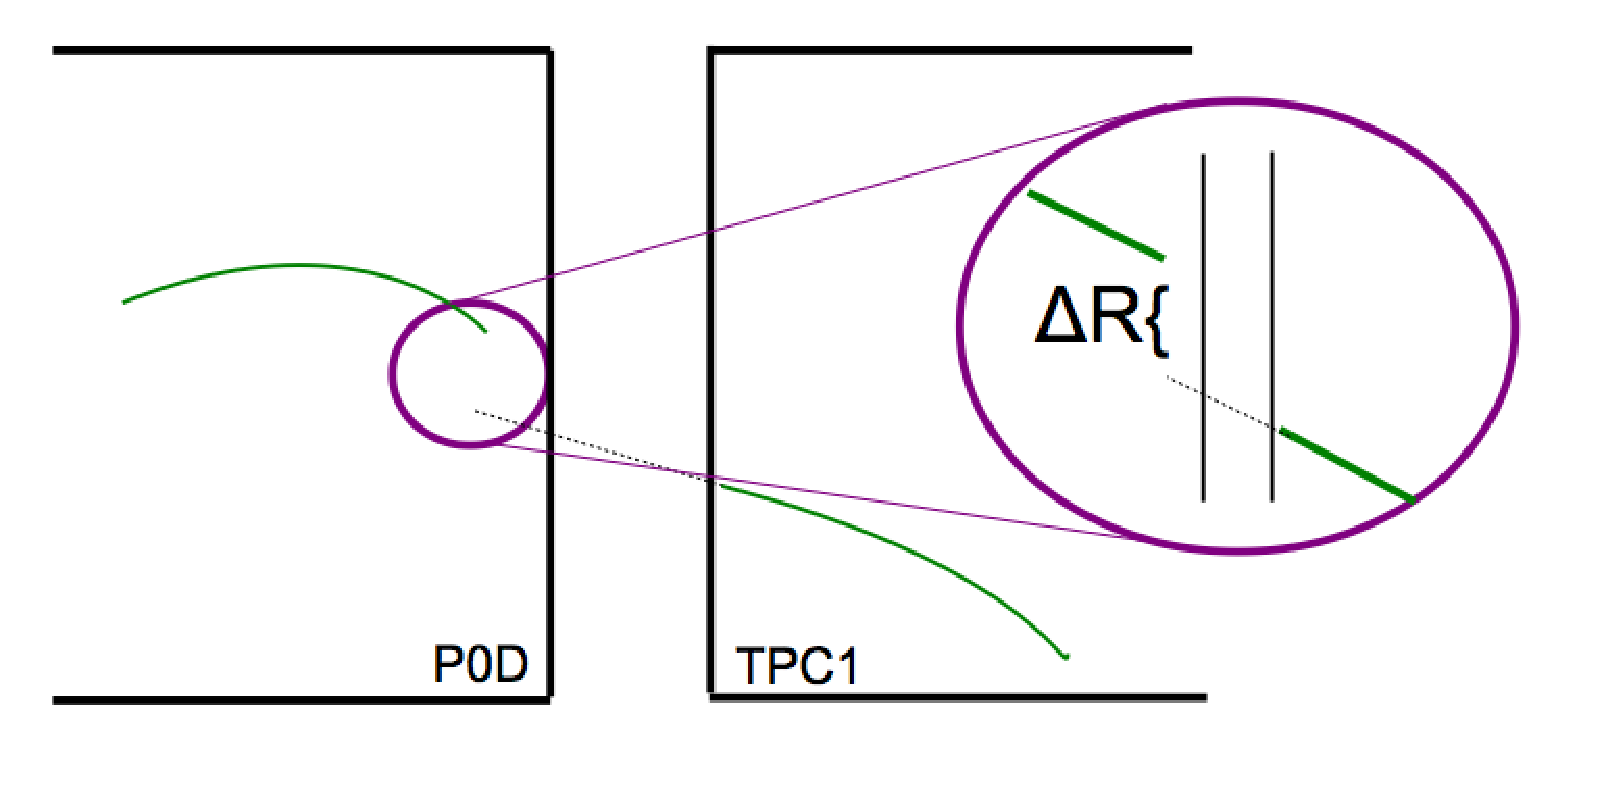
\includegraphics[width=3.2in]{Figures/drCalc.eps}
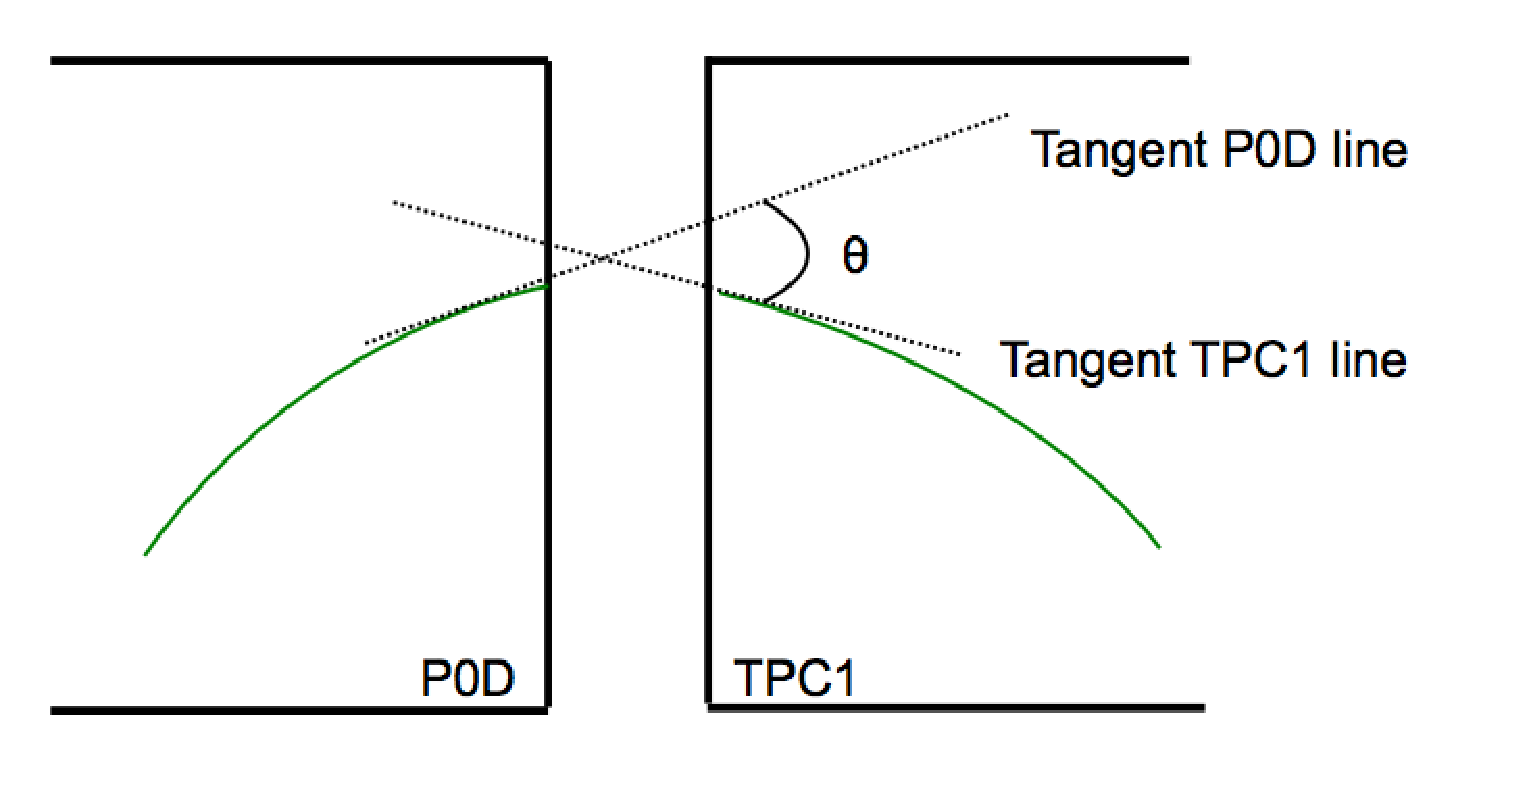
\includegraphics[width=3.2in]{Figures/sindThetaCalc.eps}
\end{center}
\caption{Graphic demonstrating how the analysis calculates $\Delta R$ (left) and sin($\Delta \theta$) (right) for the track matching algorithm.}
\label{fig:dRCalc}
\end{figure}

We use a simple figure of merit (FOM) optimization process on beam MC to determine the cut values of $\Delta$R and sin$\Delta\theta$. The chosen FOM is 
\begin{equation}
F = \frac{\delta S}{S} = \frac{\sqrt{S+2B}}{S}
\end{equation}
\noindent where S is the total number of signal events passing a certain ($\Delta$R, sin$\Delta\theta$) cut, B is the background and $\delta S$ is the error. The second form of the FOM comes from assuming poissonian errors on the total number of events and the number of background events B. Minimizing this figure of merit will maximize the total signal while minimizing the error on the signal. We use beam MC and follow the matching procedure described above up to the  ($\Delta$R, sin$\Delta\theta$) cut. For every pair of  ($\Delta$R, sin$\Delta\theta$) cut values, the signal is defined as the number of successfully matched tracks that have both track segments originating from the same primary true trajectory (a primary trajectory is a true particle vector leaving the original vertex). Then the background is the remainder of the tracks that were matched but were not from the same primary trajectory. A 3D FOM histogram is created (see Figures \ref{fig:FOM1} and \ref{fig:FOM2}) where each bin (i,j) is filled with the calculated FOM from the matching algorithm with cuts $\Delta$R$\leq$i and sin$\Delta\theta\leq$j. 

\begin{figure}
\begin{center}
\includegraphics[width=6in]{Figures/FOM1.png}
\end{center}
\caption{The figure of merit value as a function of $\Delta$R and sin$\Delta\theta$ cut values using run 2 water-in MC. The left side shows the entire allowed cut region and the right side is zoomed in to the local maximum (76~mm, 0.88) with the Z axis zero suppressed.}
\label{fig:FOM1}
\end{figure}

\begin{figure}
\begin{center}
\includegraphics[width=6in]{Figures/FOM2.png}
\end{center}
\caption{The figure of merit value as a function of $\Delta$R and sin$\Delta\theta$ cut values using run 3 water-out MC. The left side shows the entire allowed cut region and the right side is zoomed in to the local maximum (78~mm, 0.90) with the Z axis zero suppressed.}
\label{fig:FOM2}
\end{figure}

The FOM does not vary wildly over the scanned cut values. In fact, we have to zoom into the optimal region to even see where the local maxima is located. These maxima are shown in the right hand histogram in Figures \ref{fig:FOM1} and \ref{fig:FOM2}. They are at the coordinates (76~mm, 0.88) and (78~mm, 0.90) for water-in and water-out samples respectively. To simplify the selection procedure, we use the more stringent of the two cut choices, specifically $\Delta$R $\leq$ 76~mm and sin$\Delta\theta\leq0.88$ for all data and MC samples. Finally, we also investigate the agreement between data and MC in the distributions of the matching parameters. Large differences in the $\Delta$R and sin$\Delta\theta$ distributions of data and MC would cause a systematic difference in our data and MC selection efficiencies. This effect is accounted for by detailed systematic studies on the matching efficiency conducted in Section \ref{sec:matchingsyst}, but we also show in Figures \ref{fig:matchpar1} and \ref{fig:matchpar2} that the pre-cut data and MC distributions of $\Delta$R and sin$\Delta\theta$ track each other quite well near the cut values. Note that as the MC we use does not simulate external interactions, we apply a loose vertex position cut ($Z>$ -3183~mm, $|X|$ and $|Y|<$ 1000~mm) on the data.

\begin{figure}
\begin{center}[h]
\includegraphics[width=6in]{Figures/matchpar1.png}
\end{center}
\caption{The pre-cut $\Delta$R (left) and sin$\Delta\theta$ (right) distributions for data (black) and MC (red) using run 2 water-in samples.}
\label{fig:matchpar1}
\end{figure}

\begin{figure}[h]
\begin{center}
\includegraphics[width=6in]{Figures/matchpar2.png}
\end{center}
\caption{The pre-cut $\Delta$R (left) and sin$\Delta\theta$ (right) distributions for data (black) and MC (red) using run 3 water-out samples.}
\label{fig:matchpar2}
\end{figure}

\subsection{Track Momentum Reconstruction}
\label{sec:momrecon}

To reconstruct the momentum of the muon track, we use the momentum measurement from TPC1 made by fitting a helix to the track and comparing the curvature to the local magnetic field. This momentum is then corrected for the segment of the track that passed through the P0D. Using muon range tables in conjunction with the known materials density in the different P0D regions, we can calculate the momentum of the muon at the vertex by adding in the total energy lost. As we must do this for every single muon-like negative track in every event, we require that the algorithm is fast. So we chose not to use $\frac{dE}{dx}$ tables to incrementally restore the energy lost. Instead, the P0D energy loss was calculated using range data for the two types of superP0Dules: water target and ECAL. Range is defined as
\begin{equation}
R(E') = \int^{E'}_{0} \left(\frac{dE}{dx}\right)^{-1} dE
\end{equation}
where $\frac{dE}{dx}$ is the weighted average energy loss over all materials. The range is calculated for each superP0Dule. This gives us a table of range vs energy/momentum for each section of the P0D and avoids performing the integration every single time a track is found. The track length in the P0D is used to find the corresponding energy lost (see Figure \ref{fig:eloss}) and add it to the TPC1 measurement momentum. If the track traversed through mutiple superP0Dules, as it must, then the energy loss look-up procedure is performed separately for each. The momentum residual as defined by $(P_{reco}-P_{truth})/P_{truth}$ for run 2 water-in and run 3 water-out samples is shown in Figure \ref{fig:momres} for reference. The algorithm does an excellent, unbiased job of reconstructing muon momenta according to MC.

\begin{figure}
\centering
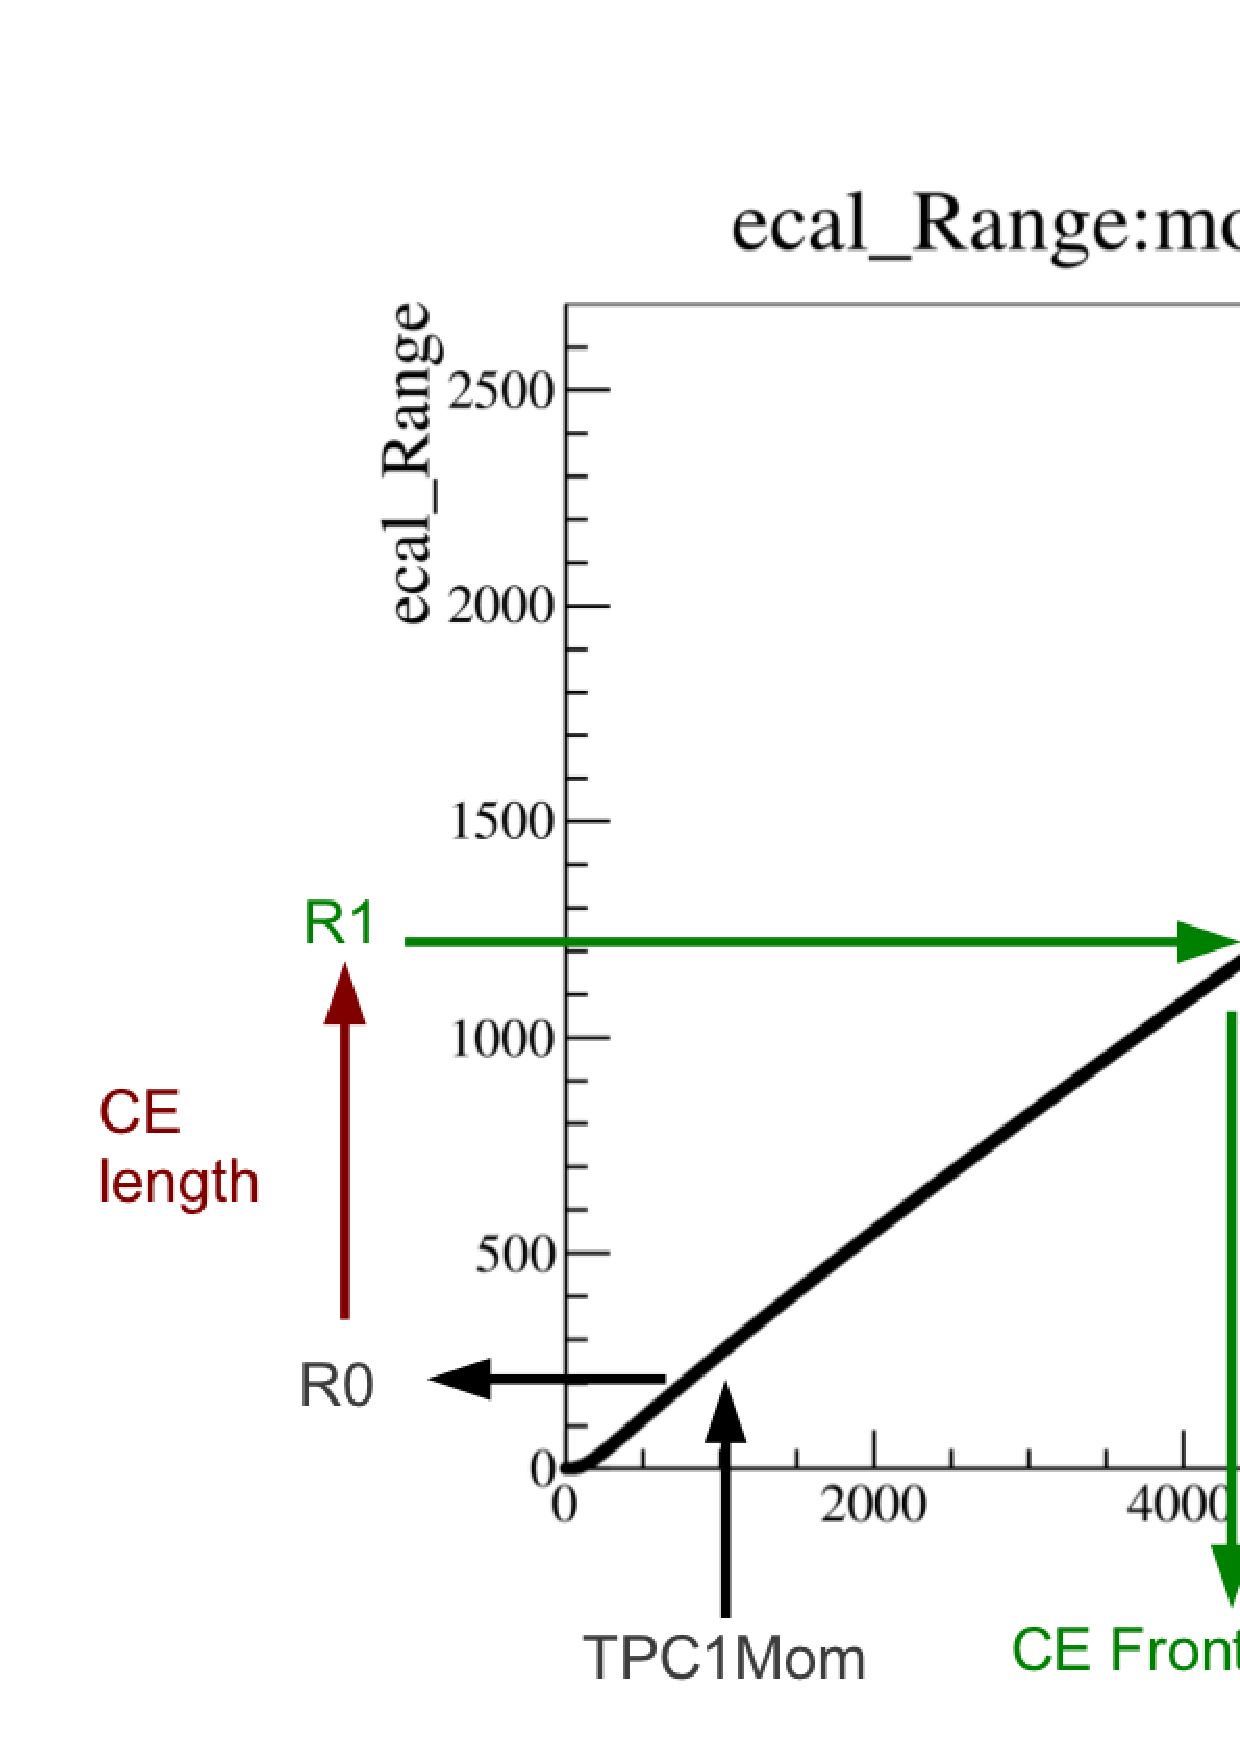
\includegraphics[width=5.5in]{Figures/eLossCalc1.png}
\caption{Calculation of P0D momentum correction. The steps of the correction
are shown schematically with the arrows} 
\label{fig:eloss}
\end{figure}

\begin{figure}
\centering
\includegraphics[width=5.5in]{Figures/momentumresidual.png}
\caption{The momentum residual comparing the reconstructed momentum with the true track momentum in run 2 water-in MC (blue) and run 3 water-out MC (purple).}
\label{fig:momres}
\end{figure}

\clearpage
\section{Fiducial Mass and Volume}
\label{sec:fidmassvol}

To calculate the $\nu_\mu$ inclusive charged current cross section, proper evaluation of the number of target nucleons is of paramount importance. This requires a clear description of an analysis fiducial volume and the measurement of the mass contained in said volume. The determination of the fiducial volume was made based on the design of the detector and the requirements of analyses predominantly concerned with selecting electromagnetic showers. Table \ref{tab:FV} lists the fiducial volume boundaries used in most analyses using the P0D. They are chosen to minimize the uncertainty on the water mass enclosed in the water target and are placed around 25~mm from the X and Y edges of the detector. These boundary values as well as all future coordinates are given with respect to the ND280 coordinate system shown in Figure \ref{fig:nd280geom}. The Z direction boundaries are chosen to primarily enclose all the water layers in the P0D. More specifically, they are placed between the X and Y layers of the two p0dules that bound the upstream and downstream ends of the water target. Since there are lead radiators in the ECALs that sandwich the water target and the interaction rates on lead are not well known, this Z axis range allows us to reject unwanted lead events while efficienctly selecting water events. 

\begin{table}[h]
\caption{The P0D Water-Target Fiducial Volume boundaries given in the ND280 coordinate system. All units are in mm.}
\centering
\begin{tabular}{ccc}
\toprule
Axis & FV (min) & FV (max) \\
\hline
X & -836 & 764 \\
Y & -871 & 869 \\
Z & -2969 & -1264 \\
\bottomrule
\end{tabular} 
\label{tab:FV} 
\end{table}

The fiducial mass of the non-water components of the P0D was determined from careful measurements during the construction of the detector. This work was completed by a few group members to provide a baseline for all P0D based analyses. We summarize the procedure and results from their work. The measurements are made for four separate elements of the P0D: brass radiators, upstream water target cover, p0dules and water. The thickness of the brass radiator sheets was measured prior to assembly and the standard density of brass used to calculate the mass. Water target covers are present to provide structural support to the outer water bag layers and are made of high-density polyethylene (HDPE). The thickness of these covers was provided by the manufacturer and the density was averaged from an online list of HDPE densities.

Each p0dule is constructed from two light-tight covers, two scintillator planes, 260 wavelength-shifting (WLS) fibers and three layers of epoxy to hold it all together. The mass of the light-tight covers was calculated by measuring their thickness and using an online list of density. The mass of each scintillator plane was measured during construction and the areal density was calculated using the total mass and fiducial area. The design thickness of each epoxy layer was used in conjunction with the known density of epoxy to calculate the mass of the three epoxy layers. Finally, the mass of the WLS fibers was calculated from the diameter and density extracted from the design specifications. The WLS fibers cross the entire height and width of the fiducial volume so the X and Y ranges were used for the fiber length. The errors on the non-water fiducial mass stem primarily from the thickness measurements and the scale used to weigh the P0Dules. They are combined by treating each component mass error as independent.

The MC fiducial mass does not use any of these specific measurements directly. Instead, the ND280 simulation geometry is density averaged and this average is multiplied by the fiducial volume. Table \ref{tab:aden} summarizes the areal density of the three non-water components of the P0D. It is important to note here that our analysis ideally subtracts out the event rate from non-water elements of the P0D. The target number in the cross section formula does not depend on the non-water fiducial mass whatsoever. This information is stated primarily for completeness.

\begin{table}[h]
\caption{The areal density of three of the four major elements of the P0D in the fiducial volume. All units are in gm/cm$^2$.}
\centering
\begin{tabular}{ccc}
\toprule
Material & Data Areal & MC Areal\\
& Density (g/cm$^2$) & Density (g/cm$^2$) \\
\midrule
Brass & $1.088 \pm 0.032$ & 1.09 \\
WT Cover & $0.024 \pm 0.002$ & 0.02 \\
P0Dule & $3.843 \pm 0.034$ & 3.84 \\
\bottomrule
\end{tabular} 
\label{tab:aden} 
\end{table}

The final component of the P0D in the fiducial volume is water. As this is our cross section target, this is also the most crucial measurement. All measurement errors translate directly to uncertainties on the cross section, so the treatment of systematics is also very important. To fill the P0D, water is pumped from a main holding tank through fill pipes and into the water bags located in the water target. The external water tank is equipped with a depth sensor and a sight glass mounted to monitor the water level inside. To measure the amount of water in the fiducial volume of the water target, the sight glass is used to observe the change in water level over the fill period and the height change is converted to water mass. This water mass is then corrected for any losses during the fill procedure and scaled down to the fiducial volume. The fiducial mass of the water ($M_{fid}$) is given by:
\begin{equation*}
M_{fid} = (C_{dm}\times H_{fid} - M_{drip} - M_{config} - M_{overshoot}) \times R_{x~cut}
\end{equation*}

Here, $C_{dm}$ is a factor that converts water level change in the main tank to water mass and $H_{fid}$ is the height change of the water in the tank over the fill period. The terms $M_{drip}$, $M_{config}$ and $M_{overshoot}$ are corrections for losses of water while filling, configuration changes in the water system and overfilling the fiducial volume respectively. To determine $C_{dm}$, 80~L buckets of water were filled from the main tank while using the sight glass to record the change in water level from each bucket fill. The water mass in the bucket was measured using a 100~kg digital scale calibrated with precision, $20$~kg$\pm 1$~g weights. The measured masses of the water buckets were plotted against the change in height of the water level. Some of the data points were rejected due to depth sensor readings that were inconsistent with the height change. The multiplicative height to mass conversion term $C_{dm}$ is the mean of the remaining data points. From two calibration runs, the $C_{dm}$ vaue is $1.0696 \pm 0.0077$~kg/mm. The data from one such calibration run is shown in Figure \ref{fig:cdm}. The sources of error on $C_{dm}$ are a $5\%$ instrument error from the weighing scale and a 2~mm uncertainty from the sight glass.

\begin{figure}
\centering
\includegraphics[width=3.2in]{Figures/cdmline.png}
\includegraphics[width=3.2in]{Figures/cdmhist.png}
\caption{Left: Measured water mass in each bucket vs. sight glass depth reading for the first of two calibration runs. The red points were rejected due to inconsistency between sight glass and main tank depth sensor readings. Right: A histogram of the ratio of measured water mass and the change in water depth after the faulty data points were removed. The mean of the remaining data points is used as the $C_{dm}$ value.}
\label{fig:cdm}
\end{figure}

Calibration fill runs were performed to evaluate the water level change ($H_{fid}$) expected when filling the fiducial volume with water. Each water bag in the P0D is equipped with a depth sensor. The bags were systematically filled a little at a time until the average depth readings over all bags equaled the lower fiducial Y boundary. The location of the water level in the main tank was marked. Similarly, the bags were filled to the upper Y boundary of the fiducial volume and another mark was placed on the main tank. The distance between these two marks is used for the water level height change $H_{fid}$. 

There are three corrections to the initial water fiducial mass calculation. The first correction, $M_{drip}$ accounts for water lost from dripping or spillage during the filling process. The total amount is very small and is estimated conservatively by eye to be $4\pm1$~kg. The second correction comes from a change in the water system configuration made after the initial main tank calibrations. An updated pumping system causes a loss in the amount of water delivered to the water bags from the main tank. This loss, $M_{config}$ is estimated to be $10\pm2$~kg. The final correction attempts to adjust for an inaccuracy in the main tank fiducial volume fill marks. The two marks on the main tank were placed by filling water bags until the \emph{average} water level in each bag was at the fiducial volume boundaries. However, it is nearly physically impossible to fill the bags to exactly where the fiducial boundaries are, so in reality the average was around 1.5~cm above the Y fiducial boundary. The correction was calculated by adding together the individual bag depth readings and comparing this to the nominal cumulative depth expected from the fiducial volume. Overfilling the bags by 1.5~cm on average corresponds to a difference of $823\pm48$~mm of water, which is $23\pm2$~kg of water. This is the value used for the $H_{overshoot}$ correction term. 

The final term in the fiducial mass equation is a multiplicative factor $R_{x~cut}$ that scales the fiducial mass down to account for the X directional boundaries. There is a vertical supportive strut in the middle of each water bag layer that separates the two water bags in each layer. Removing the width of this strut, the total width in the X direction of the water bags is $1995\pm5$~mm and the width of the fiducial volume is $1585\pm5$~mm. The ratio of the two widths is $0.794\pm0.003$ and is used as the value of $R_{x~cut}$. All the errors are treated as independent, so the final water fiducial mass with errors added in quadrature is:

\begin{equation}
M_{fid} = 1902 \pm 16 (0.8\%)~kg
\end{equation}

Now we are able to calculate the total number of target nucleons for the cross section formula. A simple calculation using Avogadro's constant and the molar mass of water yields $T_w$, the total number of nucleons in the water fiducial mass.
\begin{equation}
\label{eqn:tarnum}
T_w = \frac{6.022141\times10^{23}}{\text{mol}}\times \frac{\text{mol}}{18.015~g} \times \frac{18~\text{nucleons}}{H_2 O molecule} \times 1902~\text{kg} = 1.145 \times 10^{30} \text{nucleons}
\end{equation}


\clearpage
\section{Selection of Charged Current Inclusive Events}
\label{sec:selectionheader}

To measure the charged-current inclusive cross section on water, we must find good neutrino interaction data, clearly define the signal we are searching for and then apply a selection to determine CC inclusive event rates in the data. In the first step, we identify several, high-quality data and MC samples from the P0D corresponding to water-in and water-out configuration. Then we define what we consider a CC inclusive signal and finally we apply a cut-based selection to extract this signal from data and MC samples. This process is described in detail below and also in Ref~\cite{tn80}. While the data collection and MC generation was done by T2K as a whole, the event selection was entirely our work.

\subsection{Data and Monte Carlo Samples}
\label{sec:Samples}

This analysis uses data collected by the T2K experiment from Jan 2010 to Feb 2013. The three years of data are divided into four beam runs, each run boasting greater beam stability and intensity than the last. As the P0D was designed to be drained of water and filled with water at any time, the data taking is also divided into water-in periods and water-out periods. The P0D ran with water in during beam run 1 and with water out for beam run 3. For beam runs 2 and 4 the P0D collected both water-in and water-out data. Whether to take water-in or water-out data was decided according to various analysis needs where an attempt was made to collect equal quantitites of events for both modes.

We also consider the overall usability of collected data. The health and stability of the experimental apparatus is closely monitored both at the neutrino beam complex and the near detector facility. Any errors stemming from malfunctions or abnormal deviations in the beam setup, the near detectors or the data acquisition system are logged. These logs, both automatically and manually generated, are converted into data quality flags for each beam spill. Only events occurring within a beam spill with no bad data quality flags are used in this analysis.

The total accumulated protons-on-target (POT) for each beam run is recorded in Tables \ref{tab:DataSamplesRun1Run2Run4} and \ref{tab:DataSamplesRun2airRun3airRun4air} for water-in and water-out running respectively. The total useable POT from each of these runs is also shown. Very little data was lost to data quality issues.

\begin{table}[h]
\centering
\caption{The POT values available and used in the data analysis for 
the water-in run periods}
\begin{tabular}{cccc}\toprule
\multirow{2}{*}{Data Set} & \multirow{2}{*}{Run Period} & \multicolumn{2}{c}{Protons On Target}\\
 & & Total (Available) & DQ (Used) \\
\hline
Run 1 & Jan 2010 - Jun 2010 & $3.033\times 10^{19}$ & $2.946 \times 10^{19}$\\ 
Run 2 & Nov 2010 - Feb 2011 & $6.974\times 10^{19}$ & $4.286 \times 10^{19}$\\ 
Run 4 & Oct 2012 - Feb 2013 & $16.45\times 10^{19}$ & $16.24 \times 10^{19}$\\ 
\hline
Total &  & $26.46 \times 10^{19}$ & $23.47 \times 10^{19}$ \\ 
\bottomrule
\end{tabular} 
\label{tab:DataSamplesRun1Run2Run4} %FIXME
\end{table}

\begin{table}[h]
\centering
\caption{The POT values available and used in the data analysis for 
the water-out run periods}
\begin{tabular}{cccc}\toprule
\multirow{2}{*}{Data Set} & \multirow{2}{*}{Run Period} & \multicolumn{2}{c}{Protons On Target}\\
 & & Total (Available) & DQ (Used) \\
\hline
Run 2 & Feb 2011 - Mar 2011 & $3.593\times 10^{19}$ & $3.552 \times 10^{19}$\\ 
Run 3 & Apr 2012 - Jun 2012 & $13.58\times 10^{19}$ & $13.48 \times 10^{19}$\\ 
Run 4 & Feb 2013 - Aug 2013 & $16.37\times 10^{19}$ & $15.86 \times 10^{19}$\\ 
\hline
Total &  & $33.54 \times 10^{19}$ & $32.89 \times 10^{19}$ \\ 
\bottomrule
\end{tabular} 
\label{tab:DataSamplesRun2airRun3airRun4air} %FIXME
\end{table}

Similar to the real data, MC simulation is also divided into water-in and water-out P0D run modes. While an attempt has been made to generate as much simulated data as possible, resource constraints allow us to generate roughly an order of magnitude more events than exists in real data. However, the statistical power of the MC is assumed to be great enough to neglect statistical uncertainties from predictions made using the simulation with finite statistics. Primarily, the signal efficiencies and backgrounds that are estimated from the simulation do not have any statistical error assigned to them in the final measurement. As the size of the final statistical uncertainty is very small in comparison to the size of systematic errors, this approximation is very good. The calculation of statistical and systematic errors and a more detailed discussion of their relative sizes is included in following sections.

Finally, the Monte Carlo sample attempts to mimic the near detector setup and the beam power used for each run and so we have separate Monte Carlo samples for each run. Beam run 1 for example has no P0DEcals installed and therefore requires a different detector geometry be used in the simulation software. Also the beam intensity is greatly increased in beam run 4 when compared to beam run 1, so this also requires separate simulation. The singular exception to this rule is the water-out simulation of beam run 4. There is no existing MC simulation for the run 4 water-out sample, so we use the closest approximation. Beam run 3 uses a beam intensity that is very close to run 4. Also the detector geometries in run 3 and run 4 are identical. So we simply re-normalize the water-out run 3 MC sample to the correct protons-on-target (POT) value for water-out run 4 data and recycle the sample. 

The total simulated Protons on Target for each Monte Carlo sample is listed in Tables \ref{tab:MCSamplesRun1Run2Run4water} and \ref{tab:MCSamplesRun1Run2Run4air}. The simulated samples are all good data quality events by design.

\begin{table}[h]
\centering
\caption{The available water-in MC samples and their corresponding 
POT used for the water-in analysis}
\begin{tabular}{cc} \toprule
MC Configuration & Protons On Target \\
\hline
Run 1 & $55.10 \times 10^{19}$ \\ 
Run 2 & $75.15 \times 10^{19}$ \\ 
Run 4 & $496.2 \times 10^{19}$ \\ 
\hline
Total & $625.4 \times 10^{19}$ \\ 
\bottomrule
\end{tabular} 
\label{tab:MCSamplesRun1Run2Run4water} %FIXME
\end{table}

\begin{table}[h]
\centering
\caption{The available water-in MC samples and their corresponding 
POT used for the water-in analysis}
\begin{tabular}{cc} \toprule
MC Configuration & Protons On Target \\
\hline
Run 2 & $99.55 \times 10^{19}$ \\ 
Run 3 & $161.1 \times 10^{19}$ \\ 
\hline
Total & $260.6 \times 10^{19}$ \\ 
\bottomrule
\end{tabular} 
\label{tab:MCSamplesRun1Run2Run4air} %FIXME
\end{table}

\subsection{Signal Definition}
\label{sec:SignalDefinition}

We are using the P0D and the Tracker to make a measurement of the $\nu_\mu$ induced CC inclusive cross section on water. We primarily use a cut-based technique where events collected during beam uptime are separated into signal and background classifications. The signal events we are searching for are very specific and must satisfy the following requirements:

\begin{itemize}
\item Event is generated by the $\nu_\mu$ component of the beam.
\item Event is a Charged Current inclusive interaction
\item Event vertex is contained within the P0D fiducial volume (defined in Section \ref{sec:fidmassvol}).
\end{itemize}

Though the cross section is a measurement on water, we do not define non-water interactions as background. This is so we can use the statistical subtraction method outlined in Section \ref{sec:xsec}. Hence we select all signal events described above in both water-in and water-out P0D running. These event rates are corrected with the MC predicted background and signal efficiency for all CC inclusive events in the fiducial volume and then subtracted to extract the absolute water cross section. This technique reduces many systematic errors as we have a data-driven method for subtracting the non-water neutrino event background.

We search for the muons produced from CC inclusive events by using the Tracker. As the P0D is 2.4~m in length, and the muon track must travel through it to enter the Tracker, we are necessarily selecting a more forward going and higher momentum set of muons compared to all the $\nu_\mu$ induced CC inclusive interaction muons produced in the P0D. However, we do not add any angular or momentum requirement in the signal definition. This implies we will evaluate very small MC signal efficiencies for steep muon tracks and for low momentum muon tracks. It follows that as this is an integrated result, for these events with low signal efficiency, we are more reliant on the MC cross section model to predict the proper efficiencies. A potential extension of this analysis is the measurement of CC inclusive event rates in the P0D fiducial volume where the muons have a steep angle and escape through the P0DEcals. 



\subsection{Event Selection Procedure}
\label{sec:selection}

Now that we have defined the signal we are searching for in ND280 and the reconstruction tools we have available, we develop a selection procedure to identify candidate $\nu_\mu$ charged current interactions. Primarily, we would like to identify the daughter muon produced by a $\nu_\mu$ charged current interaction $\nu_\mu + N \rightarrow \mu^- + X$ where X represents any particle or particles. This analysis uses neutrino events from the water-target region of the P0D where the daughter muon passes through the TPC. For the MC simulation, we use the NEUT generator. We use a cut-based selection technique and summarize the steps used:

\begin{itemize}
\item Data Quality Cuts.
\begin{enumerate}
	\item The data quality flag from the beam is good for the spill is ``good"
	\item The data quality flag from the near detector is also ``good"
\end{enumerate}
\item P0D to TPC1 Track Matching. Tracks are matched together using the algorithm described in Section \ref{sec:matching}.
\item Muon Tagging:
\begin{enumerate}
	\item Sort matched tracks by time stamp into 6 or 8 beam bunches depending on beam run.
	\item Evaluate the initial momentum of each matched track under a muon hypothesis. We use the Tracker measured momentum and correct for MIP-like energy loss in the P0D to evaluate the momentum. The exact method for this momentum calculation is described in Section \ref{sec:momrecon}.
	\item Select the highest momentum, negative track in each bunch in a fiducial volume slightly larger than nominal (FV+) as the muon candidate. The charge measurement comes from the Tracker. 
	\item Apply a nominal fiducial volume (FV) cut to the most upstream position of the P0D track requiring it to be within the official P0D water target fiducial volume. The volume boundaries of FV+ and FV are shown in Table \ref{tab:WTFV}.
\end{enumerate}
\end{itemize}

We also have an additional veto to filter out a specific type of background called ``sand muons". These backgrounds are discussed in great detail in Section \ref{sec:sandintsys}. Sand muons are negative MIP-like particles that are generated in the sand and concrete outside the ND280 and then pass through part of the detector. We also define negative MIP-like particles originating in the magnet yoke and the magnet coil as sand muons. These are clearly background as they are generated outside the fiducial volume, but they require special treatment. Since they are product of beam neutrino interactions, their timing structure mimics that of a signal event. They are also negative and MIP-like, so can easily be mistaken for a signal muon. Finally, sand muons are very poorly simulated, meaning that using MC to predict the sand muon background will not work. So we have found a way of achieving high sand muon exclusion rates by using the region of the P0D outside the fiducial volume to self-veto sand muon events.

\begin{itemize}
\item Sand Muon Veto:
\begin{enumerate}
	\item Count the number of external sand muon tracks entering the P0D. This is done by searching for Kalman fitted tracks in the P0D that begin outside the FV+ volume and end inside a similar volume that is slightly smaller in the Z-direction (FV-). The volume boundaries of FV- is shown in Table \ref{tab:WTFV}.
	\item If there is a concurrent sand muon in the same bunch as a candidate muon track, we veto the entire bunch. This accounts for possible reconstruction failures where a broken sand muon track is identified as a potential muon track beginning in the nominal FV. This is shown in Figure \ref{fig:smveto}.
\end{enumerate}
\end{itemize}

\begin{table}[h]
\caption{The P0D Water-Target Fiducial Volumes used in this analysis. The nominal fiducial volume cut (FV) is applied to all events. The other two volumes (FV+) and (FV-) are used in the process of selection. All units are in mm.}
\centering
\begin{tabular}{ccccccc}
\toprule
Axis & FV (min) & FV (max) & FV+ (min) & FV+ (max) & FV- (min) & FV- (max) \\
\hline
X & -836 & 764 & -988 & 910 & -988 & 910\\
Y & -871 & 869 & -1020 & 1010 & -1020 & 1010\\
Z & -2969 & -1264 & -3139 & -900 & -3139 & -987\\
\bottomrule
\end{tabular} 
\label{tab:WTFV} 
\end{table}

\begin{figure}[h]
\centering
\includegraphics[width=6in]{Figures/smveto.png}
\caption{Graphic showing the two fiducial volume cuts used to veto sand muons. The ``Corridor" (red) boundary is the FV+ volume and the ``Corridor-" (green) boundary is the FV- volume. The external, entering sand muon track that stops in the P0D (left) causes a veto of a candidate CC inclusive event. The external, passing through sand muon track (right) does not cause a veto.}
\label{fig:smveto}
\end{figure}


\subsection{Event Selection Results}
\label{sec:selresults}

The results of the selection and the event reduction are plotted for different runs in Figures \ref{fig:xs1run1water} to \ref{fig:xs2run4air}. We also include the signal efficiency as a function of each variable. The efficiency is calculated as
\begin{equation}
\epsilon = \frac{\text{\# selected signal evts.}}{\text{\# total signal evts}}.
\end{equation}
\noindent We expect the total signal event rates to not vary as a function of the XY vertex position, so it is sensible that the signal efficiency shape mimics the event rate distribution. To first order, the data and MC reasonably track one another in the 1-D vertex distributions, though there is a discrepancy in the overall normalization. The momentum and theta distributions are a lot more interesting as they show very clearly the limitations of this selection. Specifically, we are sensitive to the higher momentum, forward-going muons and lose a lot of the steeper, low-energy muon tracks. 

\begin{figure}[h]
\centering
\includegraphics[width=3in]{Figures/TN100Plots/c_Pwater_1.png}
\includegraphics[width=3in]{Figures/TN100Plots/c_Thwater_1.png}
\includegraphics[width=3in]{Figures/TN100Plots/c_Xwater_1.png}
\includegraphics[width=3in]{Figures/TN100Plots/c_Ywater_1.png}
\caption{Kinematic and Vertex position distributions for selected events in run 1 water-in data. The data with error is shown with blue crosses and the MC signal and background are shown in red and black respectively. Below each distribution histogram is the MC predicted signal efficiency as a function of the same variable.}
\label{fig:xs1run1water}
\end{figure}

\begin{figure}[h]
\centering
\includegraphics[width=3in]{Figures/TN100Plots/c_Pwater_2.png}
\includegraphics[width=3in]{Figures/TN100Plots/c_Thwater_2.png}
\includegraphics[width=3in]{Figures/TN100Plots/c_Xwater_2.png}
\includegraphics[width=3in]{Figures/TN100Plots/c_Ywater_2.png}
\caption{Kinematic and Vertex position distributions for selected events in run 2 water-in.  The data with error is shown with blue crosses and the MC signal and background are shown in red and black respectively. Below each distribution histogram is the MC predicted signal efficiency as a function of the same variable.}
\label{fig:xs1run2water}
\end{figure}

\begin{figure}[h]
\centering
\includegraphics[width=3in]{Figures/TN100Plots/c_Pwater_4.png}
\includegraphics[width=3in]{Figures/TN100Plots/c_Thwater_4.png}
\includegraphics[width=3in]{Figures/TN100Plots/c_Xwater_4.png}
\includegraphics[width=3in]{Figures/TN100Plots/c_Ywater_4.png}
\caption{Kinematic and Vertex position distributions for selected events in run 4 water-in.  The data with error is shown with blue crosses and the MC signal and background are shown in red and black respectively. Below each distribution histogram is the MC predicted signal efficiency as a function of the same variable.}
\label{fig:xs1run4water}
\end{figure}

\begin{figure}[h]
\centering
\includegraphics[width=3in]{Figures/TN100Plots/c_Pair_2.png}
\includegraphics[width=3in]{Figures/TN100Plots/c_Thair_2.png}
\includegraphics[width=3in]{Figures/TN100Plots/c_Xair_2.png}
\includegraphics[width=3in]{Figures/TN100Plots/c_Yair_2.png}
\caption{Kinematic and Vertex position distributions for selected events in run 2 water-out. The data with error is shown with blue crosses and the MC signal and background are shown in red and black respectively.  Below each distribution histogram is the MC predicted signal efficiency as a function of the same variable.}
\label{fig:xs2run2air}
\end{figure}

\begin{figure}[h]
\centering
\includegraphics[width=3in]{Figures/TN100Plots/c_Pair_3.png}
\includegraphics[width=3in]{Figures/TN100Plots/c_Thair_3.png}
\includegraphics[width=3in]{Figures/TN100Plots/c_Xair_3.png}
\includegraphics[width=3in]{Figures/TN100Plots/c_Yair_3.png}
\caption{Kinematic and Vertex position distributions for selected events in run 3 water-out. The data with error is shown with blue crosses and the MC signal and background are shown in red and black respectively. Below each distribution histogram is the MC predicted signal efficiency as a function of the same variable.}
\label{fig:xs2run3air}
\end{figure}

\begin{figure}[h]
\centering
\includegraphics[width=3in]{Figures/TN100Plots/c_Pair_4.png}
\includegraphics[width=3in]{Figures/TN100Plots/c_Thair_4.png}
\includegraphics[width=3in]{Figures/TN100Plots/c_Xair_4.png}
\includegraphics[width=3in]{Figures/TN100Plots/c_Yair_4.png}
\caption{Kinematic and Vertex position distributions for selected events in run 4 water-out. The data with error is shown with blue crosses and the MC signal and background are shown in red and black respectively. Below each distribution histogram is the MC predicted signal efficiency as a function of the same variable.}
\label{fig:xs2run4air}
\end{figure}

\begin{figure}[h]
\centering
\includegraphics[width=2in]{Figures/TN100Plots/c_Layerwater_1.png}
\includegraphics[width=2in]{Figures/TN100Plots/c_Layerwater_2.png}
\includegraphics[width=2in]{Figures/TN100Plots/c_Layerwater_4.png}
\caption{The Z Vertex position distributions for selected events in water-in runs 1, 2 and 4 (left to right) binned by p0dule number. The data with error is shown with blue crosses and the MC signal and background are shown in red and black respectively. Below each distribution histogram is the MC predicted signal efficiency as a function of the same variable.}
\label{fig:xsZw}
\end{figure}

\begin{figure}[h]
\centering
\includegraphics[width=2in]{Figures/TN100Plots/c_Layerair_2.png}
\includegraphics[width=2in]{Figures/TN100Plots/c_Layerair_3.png}
\includegraphics[width=2in]{Figures/TN100Plots/c_Layerair_4.png}
\caption{The Z Vertex position distributions for selected events in water-out runs 2, 3 and 4 (left to right) binned by p0dule number. The data with error is shown with blue crosses and the MC signal and background are shown in red and black respectively. Below each distribution histogram is the MC predicted signal efficiency as a function of the same variable.}
\label{fig:xsZa}
\end{figure}

The event yields for data and MC are given in Table \ref{tab:sel}. For an exposure of $23.47\times 10^{19}$ POT, we select 25,419 events in water-in data. For an exposure of $32.89\times 10^{19}$ POT, we select 24,250 events in water-out data. Figures \ref{fig:xsZw} and \ref{fig:xsZa} shows the Vertex distribution and signal efficiencies for water-in and water-out runs respectively. They are binned by P0dule number which is useful for the cross section extraction outlined later. The shape of the data and MC distributions agree, however the normalization to the data compared to the NEUT MC distributions are slightly lower.

\begin{table}[h]
\caption{The total selected events from each run. The MC is normalized by POT.}
\centering
\begin{tabular}{ccc} \toprule
 & Data & MC(norm.) \\
\hline
Run 1 water-in & 3106 & 3540 \\ 
Run 2 water-in & 4652 & 5149 \\ 
Run 2 water-out & 2521 & 2967.35 \\ 
Run 3 water-out & 10077 & 11239 \\ 
Run 4 water-in & 17661 & 19678 \\ 
Run 4 water-out & 11652 & 13223 \\ 
\hline
Total water-in & 25419 & 28366\\ 
Total water-out & 24250 & 27429\\ 
\bottomrule
\end{tabular} 
\label{tab:sel}
\end{table}

\clearpage
\section{Calculating the Water Cross Section}
\label{sec:xsec}

In Section \ref{sec:selection}, highly pure samples of $\nu_\mu$ induced charged
current inclusive events were selected during water-in and water-out running
periods of the P0D. In this section, a cross
section on water is extracted by a direct subtraction of data
from water-in and water-out configurations. We use the MC
simulation to predict the background contamination in the sample and to evaluate the selection efficiency. While the flux distributions used later in this Section were taken from work done by the T2K beam group, the remainder of the cross section extraction was completed by us.

\subsection{Derivation of Statistical Subtraction Formula}

A general cross section $\sigma$~(cm$^2$/nucleon) is related to the true event rate as
follows:

\begin{equation}
N^{true} = \sigma T \Phi
\label{eqn:xsec1}
\end{equation}

where $N^{true}$ is the number of neutrino induced interactions
occurring in a volume containing $T$ total nucleons (neutrons and protons) with
a neutrino flux of $\Phi$~(cm$^{-2}$). If we know the background rate ($B$)
and efficiency ($\epsilon$) of a particular selection, then $N^{true}$ can also be
related to $N^{obs}$, the observed number of interactions:

\begin{equation}
N^{true}=\frac{N^{obs}-B}{\epsilon}.
\label{eqn:xsec2}
\end{equation}

Putting together equations \ref{eqn:xsec1} and \ref{eqn:xsec2}, we get
the general cross section formula:

\begin{equation}
\sigma = \frac{N^{obs}-B}{\epsilon \Phi T}.
\label{eqn:xsec3}
\end{equation}

We extend this simple formulation to the multi-sample, multi-target
case in the P0D. There are two types of data, water-in and water-out(air), as
well as many types of target material in the P0D. Using two versions of
equation \ref{eqn:xsec1}, we get
\begin{eqnarray}
N^{true}_1 &=& \Phi_1 \sigma_w T_w + \Phi_1 \sum\limits_{i}\sigma_i
T_i \nonumber \\
N^{true}_2 &=& \Phi_2 \sum\limits_{i}\sigma_i T_i + \Phi_2 \sigma_{air} T_{air}\nonumber
\label{eqn:xsec4}
\end{eqnarray}
\noindent where $N_1$ and $N_2$ are the total neutrino interactions in water-in
and water-out data, respectively. The cross section on air ($\sigma_{air}$) and the number of air nucleons ($T_{air}$) are both very small, so the second term in the $N^{true}_2$ equation is neglected. Since the water-in configuration of the P0D
has water and includes various other target materials, we sum up the
contributions individually. The $\Phi_1 \sigma_w T_w$ yields the
water-only contribution to the interaction rate and the $\Phi_1
\sum\limits_{i}\sigma_i$ term yields the contribution from all other
target materials summed over material type $i$. The water-out configuration
of the P0D has the exact same material types as the water-in
configuration except for air instead of water. So other than a different flux term
($\Phi_2$), the water-out equation looks similar to the water-in
equation. As we are interested in the water cross section, we solve
for $\sigma_w$, which together with equation \ref{eqn:xsec2} yields:

\begin{equation}
\sigma_w = \frac{1}{T_w}\left[\frac{N^{obs}_1-B_1}{\epsilon_1
    \Phi_1}-\frac{N^{obs}_2-B_2}{\epsilon_2\Phi_2}\right].
\label{eqn:xsec5}
\end{equation}

MC estimations of $B_1$, $B_2$, $\epsilon_1$ and $\epsilon_2$
in conjunction with the water-in and water-out selections from data then
allow us to extract the water cross section. There are a few additional considerations. As seen in Figures \ref{fig:xsZw} and \ref{fig:xsZa}, the selected number of events $N^{obs}_1$ and $N^{obs}_2$, the background terms $B_1$ and $B_2$ and the efficiency terms $\epsilon_1$ and $\epsilon_2$ are all dependent on the beam run number and the Z position of the interaction vertex. The flux terms $\Phi_1$ and $\Phi_2$ are dependent on the beam run number as the beam luminosity increased over the course of the experiment. Therefore, we rewrite the cross section equation as follows:

\begin{equation}
\sigma_w = \frac{1}{T_w}\left[\frac{1}{\sum\limits_r \Phi_1(r)}\sum\limits_{r}^{1,2,4} \sum\limits_{z}^{40} \frac{N^{obs}_1(r,z)-B_1(r,z)}{\epsilon_1(r,z)}-\frac{1}{\sum\limits_r \Phi_2(r)}\sum\limits_{r}^{2,3,4} \sum\limits_{z}^{40} \frac{N^{obs}_2(r,z)-B_2(r,z)}{\epsilon_2(r,z)}\right].
\label{eqn:xsec6}
\end{equation}

Here the Z position of the vertex is assumed to be binned according to p0dule number in the P0D. This is sensible as the expected vertex resolution in the z direction is 1 p0dule. The summation indices ``r" and ``z" correspond with beam run number and p0dule number respectively.

\subsection{Evaluating the Efficiency and Background}

An identical selection applied to the Monte Carlo simulation of P0D
data allows us to extract estimates of the selection efficiency and
backgrounds in water-in runs 1, 2 and 4 and water-out runs 2, 3 and 4. These estimates are used to correct the measured event rates in data and extract the true number of signal events in the water target. Our signal is defined as true $\nu_\mu$ induced charged
current interactions within the fiducial volume of the P0D. The backgrounds are defined as any interaction that (1) is induced by $\overline{\nu_\mu}$,
$\nu_e$, or $\overline{\nu_e}$, (2) occurs outside the fiducial volume or (3)
is non-CC. These three backgrounds are plotted as a function of P0Dule \# in Figures \ref{fig:xsbgrunw} to \ref{fig:xsbgruna}.

\begin{figure}[h]
\centering
\includegraphics[width=2in]{Figures/TN100Plots/cBG1w.png}
\includegraphics[width=2in]{Figures/TN100Plots/cBG2w.png}
\includegraphics[width=2in]{Figures/TN100Plots/cBG4w.png}
\caption{The selected background as predicted by MC and divided into three background types for run 1 water-in, run 2 water-in and run 4 water-in (left to right). The three background types are out-of-fiducial-volume (red), non-CC (black) and non-$\nu_\mu$ (blue).}
\label{fig:xsbgrunw}
\end{figure}

\begin{figure}[h]
\centering
\includegraphics[width=2.5in]{Figures/TN100Plots/cBG2a.png}
\includegraphics[width=2.5in]{Figures/TN100Plots/cBG3a.png}
\caption{The selected background as predicted by MC and divided into three background types for run 2 water-out and run 3 water-out. Note that run 4 uses the same MC files as run 3 water-out and is therefore not shown. The three background types are out-of-fiducial-volume (red), non-CC (black) and non-$\nu_\mu$ (blue).}
\label{fig:xsbgruna}
\end{figure}

\begin{figure}[h]
\centering
\includegraphics[width=3in]{Figures/BGw.png}
\includegraphics[width=3in]{Figures/BGa.png}
\caption{The selected background as predicted by MC and divided into three background types when integrated over all runs. The three background types are out-of-fiducial-volume (red), non-CC (cyan) and non-$\nu_\mu$ (dark blue). Water-in MC is to the left and water-out MC is to the right.}
\label{fig:xsbg}
\end{figure}

Figure \ref{fig:xsbg} shows the amount of background contamination as predicted by MC for water-in and water-out periods. It is separated into the three types of background types. As expected, we have a highly pure sample. The majority of the background comes from events occuring downstream of the water-target and having a vertex reconstructed inside the fiducial volume. The contribution from non-CC, non-$\nu_\mu$ and sideways entering out-of-fiducial events is extremely small. The reason we have a higher out-of-fiducial-volume (OOFV) background in the downstream end is simply because backwards going tracks do not penetrate very far into the fiducial volume. So the probability of having an event originating from downstream of the fiducial volume and having a reconstructed vertex inside the fiducial volume drops off very quickly as we move away from the downstream edge. Also, given that the selection chooses primarily forward-going muon tracks and the vertex resolution in the XY plane, contamination from OOFV background is low at the sides of the fiducial volume.

Figures \ref{fig:xsZw} and \ref{fig:xsZa} show the behavior of the selection efficiency as predicted by MC. The efficiency varies mostly due to an angular and momentum acceptance effect. We only select events that have a muon that enters the TPC downstream of the P0D. The allowed solid angle for tracks is significantly greater in the downstream region of the P0D than the upstream region. Also, the allowed range of muon momentum is greater in the downstream region of the P0D than the upstream region due to energy loss. The combination of these two effects yields a selection efficiency that varies as a function of the Z position of the interaction vertex.

As efficiency and background are both predominantly functions of the Z vertex position, we apply the efficiency correction and background subtraction also as a function of Z (see eqn. \ref{eqn:xsec6}). The reconstruction vertex resolution in Z is nominally 1 p0dule, so the selected number of events in data for each p0dule is background subtracted and efficiency corrected individually. Also, as the runs have different detector setup, beam power, etc., we also calculate the MC predicted background and signal efficiency separately for each run type and number. The end result is summed together over p0dule number, run type and run number to calculate the total true observed signal interactions in the water-target fiducial volume. The background-subtracted and efficiency-corrected ((N-B)/$\epsilon$) distributions are shown in Figure \ref{fig:xstot} for water-in and water-out. The data and MC shapes agree quite well though there is an overall normalization difference of about $15\%$. The bin contents of these 2D plots are the exact values used in Formula \ref{eqn:xsec6} for the $B_1(r,z)$, $B_2(r,z)$, $\epsilon_1(r,z)$ and $\epsilon_2(r,z)$ terms. Here the subscripts 1 and 2 correspond to water-in and water-out run types respectively. Finally, the integrated results are summarized in Table \ref{tab:xscalc}. The total MC background and signal efficiency as a function of p0dule \# for each run type and run \# is shown in Figures \ref{fig:xsBGvZ} and \ref{fig:xseffvZ}.

\begin{figure}[h]
\centering
\includegraphics[width=3in]{Figures/TN100Plots/cNBEw.png}
\includegraphics[width=3in]{Figures/TN100Plots/cNBEa.png}
\caption{The total signal binned by p0dule number for water-in runs (left) and water-out runs (right). The black crosses shows the expected signal calculated using the selected event rate in data and the MC for background and efficiency estimates. The red shows the signal according to the MC.}
\label{fig:xstot}
\end{figure}

\begin{figure}[h]
\centering
\includegraphics[width=6in]{Figures/TN100Plots/cBG_RvZ.png}
\caption{The total predicted background from MC binned by p0dule number (y-axis) and run number/type (x-axis) for all runs. The x-axis index corresponds to run 1 water-in, run 2 water-in, run 2 water-out, run 3 water-out, run 4 water-in and run 4 water-out from left to right.}
\label{fig:xsBGvZ}
\end{figure}

\clearpage

\begin{figure}[h]
\centering
\includegraphics[width=6in]{Figures/TN100Plots/cEff_RvZ.png}
\caption{The signal efficiency from MC binned by p0dule number (y-axis) and run number/type (x-axis) for all runs. The x-axis index corresponds to run 1 water-in, run 2 water-in, run 2 water-out, run 3 water-out, run 4 water-in and run 4 water-out from left to right.}
\label{fig:xseffvZ}
\end{figure}

\clearpage

\subsection{Calculating the Flux Normalization}

We calculate the total flux from the relevant flux distributions for each beam run period. The flux is integrated up to a neutrino energy of 20~GeV and then multiplied by the integrated POT corresponding to each run period. We then sum the total neutrino flux over all the run periods. Figure \ref{fig:fluxes} shows the flux distributions used for each run period.

We are not as efficient at reconstructing and selecting events generated by lower ($<1$~GeV) energy neutrinos as we are for higher energy neutrinos. This is included in the selection efficiency ($\epsilon$) as a function of P0Dule number that we use in our cross section formula. For clarity, we have included plots of the true neutrino energy distributions of the selected MC events in different runs and more importantly, the efficiency as a function of neutrino energy (Figure \ref{fig:nuEeff}).

\begin{figure}[h]
\centering
\includegraphics[width=5in]{Figures/fluxes.png}
\caption{The different flux distributions for each run.}
\label{fig:fluxes}
\end{figure}

\begin{figure}[h]
\centering
\includegraphics[width=2.5in]{Figures/TN100Plots/c_nuEwater_1.png}
\includegraphics[width=2.5in]{Figures/TN100Plots/c_nuEwater_2.png}
\includegraphics[width=2.5in]{Figures/TN100Plots/c_nuEwater_4.png}
\includegraphics[width=2.5in]{Figures/TN100Plots/c_nuEair_2.png}
\includegraphics[width=2.5in]{Figures/TN100Plots/c_nuEair_3.png}
\includegraphics[width=2.5in]{Figures/TN100Plots/c_nuEair_4.png}
\caption{The true neutrino energy of selected events in NEUT MC. The red line shows the MC total selected events, the black fill shows the background events and the blue line shows the selection efficiency as a function of true neutrino energy. The top row of plots shows MC for water-in runs 1, 2 and 4 (left to right). The bottom row shows MC for water-out runs 2, 3 and 4 (left to right).}
\label{fig:nuEeff}
\end{figure}

\subsection{Cross Section Value}

Using the integrated flux, the known volume of water in the P0D, and the total expected signal events in each run period, we can use Formula \ref{eqn:xsec6} to evaluate the central value of the absolute water cross section. For 1902~kg of water, we have $1.145\times10^{30}$ nucleons. As this is the only target, we do not need to average out nucleus type. Using the flux term calculated in the previous section and the target number above, we measure an absolute water CC inclusive cross section of:

\begin{equation}
\left<\sigma\right>_\Phi = 6.51 \times 10^{-39} \frac{cm^2}{H_2O\:nucelon}.
\end{equation}

Note that this is only the central value before any corrections due to detector biases. We will deal with shifts in the central value of the cross section in the following section. Table \ref{tab:xscalc} shows the integrated flux per POT and calculated signal (N-B)/efficiency for each run that was used to measure the absolute, uncorrected, nominal cross section. The last column shows the nominal CC inclusive cross section calculated using an estimate of 5480~kg for the total mass in the P0D fiducial volume. The exact mass of the entire fiducial volume is not as well constrained as the mass of the water. We also show the water-in and water-out CC inclusive cross sections on the P0D as a combination of materials. Before applying any of the systematic corrections, we note that water-in and water-out cross sections are very similar. This happens as carbon, the primary material in the P0D, is known to have a similar cross section to water.

\begin{table}[h]
\caption{The total calculated signal (N-B)/eff and the integrated flux per POT for each run. These values are used to calculate the uncorrected nominal cross section on water. The last column also shows an uncorrected estimation of a CC inclusive cross section for all P0D materials combined.}
\centering
\begin{tabular}{cccc} \toprule
Run & (N-B)/e & Int. Flux ($10^{13}$~$\nu_\mu$/$10^{21}$ POT) & Cr. Sec. ($10^{-39}$cm$^2$/nucleon)\\
\hline
Run 1 water-in & 11698.2 & 1.9042 & 6.32\\ 
Run 2 water-in & 17811.7 & 1.92516 & 6.54\\ 
Run 2 water-out & 9263.16 & 1.92516 & 6.29\\ 
Run 3 water-out & 37518.9 & 1.92639 & 6.71\\ 
Run 4 water-in & 68044 & 1.93972 & 6.55\\ 
Run 4 water-out & 42593.7 & 1.93972 & 6.43\\ 
\hline
Water-in & 97554 & & 6.52\\
Water-out & 89376 & & 6.53\\
\hline
\bottomrule
\end{tabular} 
\label{tab:xscalc}
\end{table}

\clearpage
\section{Systematic Uncertainties in the Flux Prediction and Cross Section Model}
\label{sec:fluxxsecsyst}

There are three major sources of systematic uncertainty in our measurement:

\begin{itemize}
\item Flux prediction uncertainty
\item Cross section model simulation uncertainty
\item Detector level uncertainties caused by imperfect detector simulation
\end{itemize}

In this section, we describe the treatment of the first two sources of uncertainty, the flux prediction and the cross section model. Section \ref{sec:FluxDetermination} outlined the methodology behind extracting the uncertainty on the netrino flux at ND280. In Section \ref{sec:fluxsyst}, we complete the treatment of the flux uncertainty by propagating it through to our cross section measurement. Similarly, Section \ref{sec:evsim} discussed the parametrization and evaluation of the cross section model uncertainties and in Section \ref{sec:xsecsyst} we propagate these through to our measurement.

\subsection{Flux Prediction Systematic Uncertainty}
\label{sec:fluxsyst}

The flux systematic uncertainty is a large source of error in the cross section measurement. The majority of the uncertainty is due to the hadronic interaction model used with some small contribution from uncertainties in the proton beam alignment/angle and the horn current and field. As described in Section \ref{sec:FluxDetermination}, the flux uncertainty is parametrized by normalization factors in bins of neutrino or anti-neutrino energy. The $\nu_\mu$ flux is divided into 11 bins, the anti-$\nu_\mu$ into 5 bins, the $\nu_e$ into 7 bins and the anti-$\nu_e$ into 2 bins. The bin limits used are as follows (in GeV):

\begin{itemize}
\item $\nu_\mu$: 0, 0.4, 0.5, 0.6, 0.7, 1.0, 1.5, 2.5, 3.5, 5.0, 7.0, 30.0
\item anti-$\nu_\mu$: 0, 0.7, 1.0, 1.5, 2.5, 30.0
\item $\nu_e$: 0, 0.5, 0.7, 0.8, 1.5, 2.5, 4.0, 30.0
\item anti-$\nu_e$: 0, 2.5, 30.0
\end{itemize}

To propagate the flux error to our measurement, we use a 25 by 25 covariance matrix that encodes the current constraints on and correlations between the flux parameters. Figure \ref{fig:fluxcov} from Section \ref{sec:FluxDetermination} shows the flux covariance matrix used with bins for each of the neutrino types for ND280 and Super-K. The 25 bins at the bottom left of the flux covariance matrix shown are the ND280 flux bins that are used, the remainder are Super-K flux bins. We use a Cholesky decomposition technique \cite{chol} on the correlation matrix and multiply the resulting lower triangular matrix with a vector of 25 uncorrelated, gaussian, random values. The gaussians are centered at 1 and have a variance equal to the known variance of the corresponding flux bin. Each random vector multiplied by the decomposed correlation matrix yields a properly correlated ``throw'' of flux bin weights. When each flux bin weight is multiplied by the integrated flux in the given bin, each throw can be thought of as a new flux prediction. So for every new flux prediction, we have to recalculate the cross section value we aim to measure, and after many repeated throws, we produce a distribution of possible cross section measurements. The variance of this distribution tells us the uncertainty in our cross section measurement due to the uncertainty in the flux prediction at ND280. The Cholesky decomposition technique is a common mathematical tool and we use an implementation of the algorithm created by a T2K collaborator. The remainder of the flux uncertainty propagation is our work.

To recalculate the cross section for each flux throw, we re-evaluate six pieces of the cross section formula in \ref{eqn:xsec6}. We re-weight the MC and recalculate the background terms, efficiency terms and integrated flux terms. The same covariance matrix is used for all 4 beam runs. To reweight the integrated flux term, we first integrate the neutrino flux within the energy range of each $\nu_\mu$ flux bin. This integrated value is multiplied by the corresponding element, $w(i)$, of the thrown 25-element vector. This yields the new neutrino flux in that particular bin. We integrate over all 11 $\nu_\mu$ bins to calculate the new total flux as follows.

\begin{equation}
\Phi_{tot} = \sum_{i}^{11} \Phi^{new}(i) = \sum_{i}^{11} \left( w(i) \int^{bin\:hi\:edge}_{bin\:low\:edge} \Phi^{old}(i) dE_\nu \right).
\end{equation}

 The efficiency reweighting is done event by event. We use the energy of the neutrino that generated each event to find its corresponding $\nu_\mu$ flux bin. This in turn gives us the event weight for a particular flux vector throw. All the selected and unselected signal events are thus reweighted and the efficiency is recalculated. The background reweighting is done similarly. As our signal definition requires that the CC inclusive event be generated by $\nu_\mu$ only, the background term has some fraction of non-$\nu_\mu$ generated events. So while we only use the first 11 elements of the thrown flux weight vector for reweighting the integrated flux and signal efficiency terms, we use all 25 for the background reweighting. We calculate a weight for each background event using the interaction neutrino's type and energy to find the corresponding element in the thrown flux vector. Then the background terms are all recalculated. We take 5000 flux throws and therefore repeat the procedure 5000 times to create a smeared distribution of the cross section prediction due to flux uncertainties. This value was selected as a compromise between computing time required and the desire for highest possible statistics.

The results of 5000 variations of the flux uncertainties on the cross section is shown in Figure~\ref{fig:fluxvar}. We integrate the distribution from either extreme to find the cross section values that correspond to 15.9\% (area under normal distribution curve from -$\infty$ to -1$\sigma$) of all throws giving values below (or above for the upper limit) it. The integrated measurement has a fractional flux systematic uncertainty of -9.62\% and +11.09\%.

\begin{figure}[h]
\centering
\includegraphics[width=5in]{Figures/fluxvar.png}
\caption{A distribution of the calculated absolute water cross section for 5000 throws of the input flux. The input flux variations are calculated directly from throws of the ND280 bins of the flux covariance matrix.}
\label{fig:fluxvar}
\end{figure}

The cross section error on just the flux term is around $12\%$. However, we measure an overall error of less that $12\%$ on the cross section due to the subtraction method used. There is a larger fraction of out-of-fiducial background in the water-out selection than in the water selection. The background terms increase linearly with total integrated flux, whereas the efficiency terms remain roughly invariant as a function of flux. When calculating total expected signal events in water-in and water-out (N-B/eff.), the final value therefore varies inversely with the integrated flux term variation. However, the total expected signal in water-in data has a smaller variation that the signal in water-out due to smaller background fraction. So in effect, the total expected signal in water-only increases as integrated flux increases and decreases as integrated flux decreases. This correlation yields a smaller error due to flux uncertainty in this subtraction method.

\subsection{Cross Section Model Systematic Uncertainty}
\label{sec:xsecsyst}

The systematic uncertainty from the cross section model is another large contributor of error in this cross section measurement. To evaluate this error, we use reweighting software called T2KReWeight. This software was developed by several T2K working groups working together, and we were not directly involved with its development. This Section covers how we use T2KReWeight to propagate external physics model uncertainties to our absolute cross section measurement. Ideally, for every small variation in a cross section parameter, the MC would be regenerated. Then the particles would be repropagated and the events reconstructed and reselected. However, this is computationally intractable. Instead, the T2KReWeight software calculates the resulting MC variations on the fly by using precalculated response functions. 

For a variation in a physics parameter, the theoretical cross section in NEUT is recalculated. The ratio of the recalculated cross section and the nominal cross section is stored. This procedure is repeated for multiple variations in each physics parameter, storing the cross section ratios for each. This is handled by the reweighting capabilities of the neutrino generator being used, in this case NEUT. Afterwards, T2KReWeight takes a MC neutrino interaction, and based on the interaction type and other truth kinematics, uses the cross section ratios to calculate an event weight that is a ``reweighting" of the nominal event. This weight is directly related to the cross section ratio and is essentially a multiplicative factor describing the change in probability of the event occurring. As the MC truth information is available at all times, event weights can be generated at any given time, without needing to reprocess terabytes of data. Furthermore, while varying parameters like $M_A^{QE}$ requires help from NEUT, most of the cross section parameters are normalization factors. These factors are basically weights already as they can be directly applied to all events from a specific interaction mode (i.e. an increase in the CCQE normalization parameter of $10\%$ means an increase in the CCQE content of our samples by $10\%$ also). This reweighting method is used to quickly evaluate the effect of cross section model uncertainties on our measurement.

 The parametrization of the cross section model and the size of the corresponding errors were discussed in Section \ref{sec:evsim}. There are two types of cross section model uncertainties that were propagated. The first type are uncertainties in the 4-vector generation at the neutrino interaction vertex and the second type are the uncertainties in interactions that occur as a generated particle travels through the nucleus. The latter type of uncertainties are referred to as Final State Interaction (FSI) errors and are evaluated separately.

To estimate the neutrino interaction cross section model uncertainties, for each parameter, we generate an event weight for each selected Monte Carlo CC inclusive event and for each unselected true Monte Carlo CC inclusive event using T2KReWeight. The re-weighted Monte Carlo events will produce a new event cross section evaluated for a 1-sigma parameter excursion divided by the nominal parameter cross section. This is done for each parameter by evaluating weights at a $\pm$1-sigma excursion. Once each selected and unselected event has a weight, we re-evaluate the MC predicted backgrounds and efficiencies and finally the cross-section. The final error for each parameter leads to a fractional shift in the nominal cross section value

\begin{equation}
\delta(\sigma) = \frac{\sigma^{var.}-\sigma^{nom}}{\sigma^{nom}}.
\end{equation}

The positive and negative errors from each parameter variation are shown in Table \ref{tab:XSecPar}. The addition of these errors is not a straightforward task however, especially as the cross section parameters themselves are correlated. Ideally, we would take a throw from the correlation matrix in Figure \ref{fig:xseccorr} for the single pion fit parameters and use gaussian throws for the rest to perform the reweighting procedure multiple times. The resulting distribution of the water cross section values would then yield a total error from physics model uncertainty. This process is unfortunately too computationally intensive, so we use a simpler method. We note that the only two parameters from the single pion fit that affect the measurement appreciably are $M_A{RES}$ and CC 1$\pi$ normalization. The other single pion parameters are either not highly correlated or do not affect the water cross section. Looking closely at the $M_A^{RES}$ parameter, we find that if it increases (decreases), the cross section value decreases (increases). On the other hand, when the CC 1$\pi$ normalization increases (decreases), the cross section value also increases (decreases). Since $M_A^{RES}$ and the CC 1$\pi$ normalization are anti-correlated, upward excursions of $M_A^{RES}$ would suggest downward excursions of CC 1$\pi$ normalization. This is consistent with the cross section decreasing only. Similarly, a downward excursion of $M_A^{RES}$ would suggest an upward excursions of CC 1$\pi$ normalization, yielding an increase in the cross section. So conservatively, we linearly add the fractional cross section change from negative excursions of both parameters. The same is done for the positive excursions. From the values in the last two columns of Table \ref{tab:XSecPar}, this results in a combined $M_A^{RES}$ and CC 1$\pi$ normalization error of $+3.57\%$ and $-3.75\%$.

The rest of the parameters are assumed completely uncorrelated. Even though upward and downward excursions of each parameter cause the cross section to change in different directions, all the remaining errors are added in quadrature. Figures \ref{fig:xsvar1} and \ref{fig:xsvar2} shows the fractional change in the signal efficiency and background rate as a function of the Z vertex position binned by p0dule number. Only water-in MC is shown as the water-out results look very similar. Each plot has the $\pm 1 \sigma$ variation results for a single standard interaction cross section parameter. As the background rate and signal efficiencies are very small in certain regimes, the fractional change varies wildly in those areas, but have little impact on the final cross section measurement. The final systematic uncertainty due to the interaction physics model is $+8.78\%$ and $-13.43\%$. 

\begin{table}[h]
\centering
\caption{Cross section model parameter uncertainties and the resulting absolute water-only cross section fractional error.}
\begin{tabular}{lcccc}\toprule\midrule
\renewcommand{\arraystretch}{1.1}
Parameter &  Value & Error & + Var. (\%) & - Var. (\%)
\\ \midrule
M$_A^{QE}$ & 1.21GeV$^2$ & 0.45 GeV$^2$ & 3.9 & -7.33\\
\midrule
M$_A^{RES}$ & 1.16GeV$^2$ & 0.11 GeV$^2$ & 0.86 & -0.89\\
\midrule
Spectral Function & off & on/off & 0 & -4.01\\
\midrule
Fermi Momentum & 217 MeV/c  & 30 MeV/c & 0.81 & -0.77\\
\midrule
Pionless Delta Decay & 0.2 & 0.2 & 0.21 & -1.05\\
\midrule
DIS/Multi-Pi Shape & 1.0 & 0.4 &  0.46 & -0.44\\
\midrule
CC QE Norm. (E$_\nu < 1.5$~GeV) & 1.0 & $0.11$ & 2.81 & -2.90\\
\midrule
CC QE Norm. (3.5~GeV$>$ E$_\nu > 1.5$~GeV) & 1.0 & $0.30$ & 1.83 & -1.73\\
\midrule
CC QE Norm. (E$_\nu > 3.5$~GeV) & 1.0 & $0.3$ & 1.75 & -1.66\\
\midrule
CC Res Norm. (E$_\nu < 2.5$~GeV) & 1.63 & $0.43$ & 2.71 & -2.85\\
\midrule
CC Res Norm. (E$_\nu > 2.5$~GeV) & 1.0 & $0.4$ & 5.65 & -4.80\\
\midrule
CC Coh Norm. & 1.0 & $1.0$ & 1.42 & -1.31\\
\midrule
%NC COh Norm. & 1.0 & $0.3$ & 0.01 & -0.01\\
%\midrule
%NC 1Pi Norm. & 1.0 & $0.3$ & 0.01 & -0.01\\
%\midrule
NC Other Norm. & 1.0 & $0.3$ & 0.24 & -0.24\\
\midrule
MiniBoone CC 1Pi E$_\nu$ Shape. & off & on/off & 0.0 & -7.45\\
\midrule
\midrule
Total Interaction Systematic & &&$+8.78\% $  & $-13.43\%$  \\
\midrule
\bottomrule
\end{tabular}
\label{tab:XSecPar}
\end{table}

\newpage
\clearpage
\begin{figure}[h]
\centering
\includegraphics[width=5in]{Figures/TN100Plots/c_6_0.png}
\caption{The fractional change in the water-in signal efficiency (predicted from MC) as a function of p0dule number of neutrino interaction vertex for a +1 $\sigma$ (blue) and -1$\sigma$ (red) variation of cross section parameter. From left to right, top to bottom, the cross section parameters varied are: MAQE, MARES, DIS Multi-Pi Shape, Spectral Function, Fermi Momentum, Pion-less Delta Decay, CCQE Norm. ($E_\nu < 1.5$GeV), CCQE Norm. ( 3.5~GeV$E_\nu>1.5$GeV), CCQE Norm ($E_\nu > 3.5$GeV), CC 1Pi Norm. ($E_\nu < 2.5$GeV), CC 1Pi Norm. ($E_\nu > 2.5$GeV), CC Coh Norm., NC Coh Norm., NC 1Pi Norm., NC Other Norm., MiniBoone CC 1Pi $E_\nu$ Shape.}
\label{fig:xsvar1}
\end{figure}

\newpage
\begin{figure}[h]
\centering
\includegraphics[width=5in]{Figures/TN100Plots/c_12_0.png}
\caption{The fractional change in the water-in background (predicted from MC) as a function of p0dule number of neutrino interaction vertex for a +1$\sigma$ (blue) and -1$\sigma$ (red) variation of cross section parameter. From left to right, top to bottom, the cross section parameters varied are: MAQE, MARES, DIS Multi-Pi Shape, Spectral Function, Fermi Momentum, Pion-less Delta Decay, CCQE Norm. ($E_\nu < 1.5$GeV), CCQE Norm. ( 3.5~GeV$E_\nu>1.5$GeV), CCQE Norm ($E_\nu > 3.5$GeV), CC 1Pi Norm. ($E_\nu < 2.5$GeV), CC 1Pi Norm. ($E_\nu > 2.5$GeV), CC Coh Norm., NC Coh Norm., NC 1Pi Norm., NC Other Norm., MiniBoone CC 1Pi $E_\nu$ Shape.}
\label{fig:xsvar2}
\end{figure}

The FSI error is evaluated following the procedure in Section \ref{sec:evsim}. There are 16 combinations of variations used for the FSI parameters to fully account for the necessary uncertainty. Each combination of 16 parameter variations is fed through T2KReWeight and the water cross section is recalculated. The fractional change from the nominal cross section is given as the error as before. The water cross section error from each combination are averaged together to yield the FSI uncertainty contribution. The results are shown in Table \ref{tab:XSecFSI}.

\begin{equation}
\sigma_{avg}^2 = \sum_i^{16} \frac{\sigma_i^2}{16}
\end{equation}

\begin{table}[h]
\caption{Final State Interaction parameter uncertainties and the resulting water-only cross section fractional error.}
\centering
\begin{tabular}{cccccccc}\toprule\midrule
\renewcommand{\arraystretch}{1.1}
Comb.& Inel Lo & Inel Hi & Pi Prod. & Pi Abs. & Ch Ex Lo & Ch Ex Hi & Error
\\ \midrule
1 & 0.6 & 1.1 & 1.5 & 0.7 & 0.5 & 2.3 & 0.23\%\\
\midrule
2 & 0.6 & 1.1 & 1.5 & 0.7 & 1.6 & 2.3 & 0.56\%\\
\midrule
3 & 0.7 & 1.1 & 1.5 & 1.6 & 0.4 & 2.3 & 0.16\%\\
\midrule
4 & 0.7 & 1.1 & 1.5 & 1.6 & 1.6 & 2.3 & 0.27\%\\
\midrule
5 & 1.4 & 1.1 & 1.5 & 0.6 & 0.6 & 2.3 & 0.45\%\\
\midrule
6 & 1.3 & 1.1 & 1.5 & 0.7 & 1.6 & 2.3 & 0.33\%\\
\midrule
7 & 1.5 & 1.1 & 1.5 & 1.5 & 0.4 & 2.3 & -0.44\%\\
\midrule
8 & 1.6 & 1.1 & 1.5 & 1.6 & 1.6 & 2.3 & -0.03\%\\
\midrule
9 & 0.6 & 2.3 & 0.5 & 0.7 & 0.5 & 1.3 & 0.46\%\\
\midrule
10 & 0.6 & 2.3 & 0.5 & 0.7 & 1.6 & 1.3 & 0.34\%\\
\midrule
11 & 0.7 & 2.3 & 0.5 & 1.6 & 0.4 & 1.3 & 0.30\%\\
\midrule
12 & 0.7 & 2.3 & 0.5 & 1.6 & 1.6 & 1.3 & 0.30\%\\
\midrule
13 & 1.4 & 2.3 & 0.5 & 0.6 & 0.6 & 1.3 & 0.30\%\\
\midrule
14 & 1.3 & 2.3 & 0.5 & 0.7 & 1.6 & 1.3 & -0.01\%\\
\midrule
15 & 1.5 & 2.3 & 0.5 & 1.5 & 0.4 & 1.3 & -0.37\%\\
\midrule
16 & 1.6 & 2.3 & 0.5 & 1.6 & 1.6 & 1.3 & -0.31\%\\
\midrule
Total & & & & & & & 0.34\%\\
\midrule
\bottomrule
\end{tabular}
\label{tab:XSecFSI}
\end{table}

The total error in the absolute water cross section measurement is +8.79\% and -13.43\% when FSI and standard interaction uncertainties are added in quadrature. We note that there is some model dependence in our measurement that is introduced through the MC estimate of the background interactions. Also, a majority of the background contamination is OOFV CC inclusive events. As this background still consists of CC inclusive events (albeit outside the fiducial volume) we are using the MC to model not only the contamination rate of the OOFV events, but also the rate of CC inclusive events. This implies that there is some signal model dependence in our measurement. As the variation of $M_A^{QE}$, a parameter that controls a signal interaction mode, caused a 7\% shift in the cross section measurement, the model dependence is not negligible.

\newpage
\section{Detector Systematic Effects}
\label{sec:detsys}

The detector related systematic uncertainty is the smallest source of systematic uncertainty in the absolute water cross section measurement. Also, there are a few corrections in detector modeling and simulation that must be applied to the cross section calculation. The sources of detector systematic uncertainty and correction are: 

\begin{enumerate}
\item P0D tracking and matching efficiency
\item Hit Reconstruction efficiency
\item Neutral back scattering
\item Fiducial volume
\item Sand muon background rate
\item Out of fiducial volume background
\item Event pile-up rate
\item Track timing
\item Cosmic background
\item TPC1 tracking efficiency
\item Charge mis-ID rate
\end{enumerate}

In the following sections we describe the evaluation of these uncertainty sources in great detail. We first evaluate the systematic uncertainties and present the results as an error on the ratio of total selected events in data to the total selected events in MC. The errors on the data/MC ratio are summarized in Table \ref{tab:syssum} following the discussion of the error calculation methodologies. With the exception of the TPC1 tracking efficiency and the charge mis-ID rate, all other work in this Section is entirely ours. The TPC1 tracking efficiency and the base charge mis-ID rates per TPC were provided to us by the Tracker group. Our contribution lies in propagating this information to an uncertainty on the absolute water cross section. 

In a subsequent section, we develop a formalism for propagation of data/MC ratio uncertainties to cross section measurement uncertainties. We also describe how we correct the cross section result for inaccuracies in the detector modeling and background simulation. Finally, the developed formalism is used in conjunction with the results from this section to yield the new central value and the detector systematic uncertainties of the absolute $\nu_\mu$ CC inclusive cross section on water.

\subsection{Track Matching Efficiency Uncertainty}
\label{sec:matchingsyst}

The efficiency of reconstruction, and the differences between Monte Carlo and data efficiencies, are the first source of systematic uncertainty studied for the CC inclusive selection. There are several steps involved in reconstructing the final candidate muon track as described in previous sections. In this section, we use a `FGD Cosmic' sample to  investigate the reconstruction and matching efficiencies of our analysis. Cosmics provide a sample independent of the physics we are probing, and are an excellent unbiased sample to use to evaluate the efficiency systematic. However, as Cosmics do not have the same bunched timing structure as our beam events, we also used as independent sample of sand muons to cross check our results. Sand muons are generated by beam neutrinos interacting with material outside the off-axis near detector and have the same timing as the beam events. The sand muon study is not shown, but efficiencies extracted from cosmics and sand muons agree well. Finally, we also performed a hand-scan of beam events in reconstruction files to identify and quantify any reconstruction issues missed with the FGD cosmics and sand muon samples.

We use a simple method to examine the efficiency of our matching algorithm for tracks that deposit energy in the P0D, enter the Tracker and are reconstructed by the Tracker reconstruction software. We simultaneously determine how often P0D reconstruction successfully fits a track and how often we succesfully match this track with a Tracker reconstructed track. First, we pre-select a sample of quality tracks reconstructed in TPC1 that point squarely into the 
P0D. We then attempt to pair each of these tracks to a P0D reconstructed track. The ratio of the number of matched pairs found to the number of quality TPC1 tracks yields the ``matching efficiency". Though this estimate is not necessarily the absolute efficiency, given that MC simulates data well to first order, the observed difference between the MC efficiency and the data efficiency gives us the systematic due to reconstruction and matching.

This definition folds in the P0D's intrinsic, lower level reconstruction efficiencies (i.e. hit finding, P0D-only tracking, etc.) as well as matching and recombination efficiencies from the matching algorithm. However, as we use reconstructed tracks in the ND280 Tracker as a baseline, we do not account for the Tracker tracking efficiency with this strategy. We determine the systematic uncertainty from the Tracker efficiency separately in a later section.

\subsubsection{Cosmics Sample}
\label{sec:CosmicsEfficiency}

Using the `FGD Cosmics' sample, we extract the matching efficiency as defined above. The following determine the denominator and numerator. Note that for the numerator of the efficiency, the cuts closely mimic those used in Section \ref{sec:selection} to select muon candidates. Also, the pre-selection cuts are slightly different between the Cosmics sample as opposed to the Sand Muon sample. The necessity for this difference is discussed later.

Pre-Selection Cuts (Denominator):

\begin{enumerate}
\item There must be a Tracker reconstructed track in the event
\item The Tracker track must be reconstructed as beginning at the upstream face of the first TPC (Z \(<\) -750 mm)
\item The TPC must measure a momentum of at least 250 MeV
\item Project the Tracker track linearly backwards into the P0D. The projection is made to the Z = -1100 mm plane, and then just the XY fiducial cut is applied to the projected point.
\item The Tracker track has \(>\) 18 reconstruction nodes
\item The Tracker track has a `corrected time' stamp between -4800ns and -4400ns. The time correction allows us to find the tracker time in relation to the P0D electronics. The time cut is placed 80ns from the edge of the 480ns-wide P0D integration window. This is the window where the P0D electronics are capable of properly reconstructing hits.
%\item There are at least 3 `good P0D hits'. A `good hit' is defined as a 7 p.e. or greater P0D hit which is found within a certain region of the P0D and with a certain time. The region we search is a cone with opening angle of 30 degrees and length of 250mm. The time is required to be 80ns from the edge of the P0D integration window. We make this cut to assure that no noise hits or hits with invalid timing due to known electronics design, are contaminating our pre-selection.
\end{enumerate}

Matching Cuts (Numerator):
\begin{enumerate}
\item All pre-selection cuts are made as above
\item P0D Vertex must be reconstructed by TP0DPairwiseVertexPID algorithm, proprietary reconstruction algorithm, and the track must be a constituent of this vertex
\item P0D Track must be exiting as defined by the last node having a Z position $>$ -1016 mm
\item P0D Track must be 3D as defined by cutting on track position variance
\item Evaluate $\Delta R$, $\Delta \sin \theta$  and $\Delta T$ between the p0d track projection and tracker track as before. Apply the following cuts: $\Delta R$ \(<\) 86mm, $\Delta \sin \theta$ \(<\) .76, $\Delta T$ \(<\) 100~ns.
\end{enumerate}

The number of tracks passing the numerator cuts divided by the number passing the denominator cuts yields the efficiency. Figures \ref{fig:eff_dR} and \ref{fig:eff_dSdT} show the matching parameter distributions for $\Delta R$, $\Delta X$, $\Delta Y$, $\sin \Delta \theta$ and $\Delta T$. 
The $\Delta Y$ distribution does not agree very well and causes some disagreement in the $\Delta R$ distribution as well. This discrepancy has been isolated to a difference between forward going and backwards going cosmics tracks as determined by the Tracker reconstruction. Figure \ref{fig:dY} shows the $\Delta Y$ residuals separated by forward and backwards going tracks for FGD cosmics in data and MC. Note that in MC, the two different directions have a small shift in the central value of the residual. However, in data, the shift is much greater. We have fit gaussians to all of the residuals and the results are shown in Table \ref{tab:FitdY}. The root cause of this effect is a difference in the geometry used for reconstruction and the geometry of the `as built' detector. Finally, note that since the $\Delta R$ agreement between data and MC for the Cosmics sample is actually worse than the beam events, the evaluated uncertainty should be conservative. 
Similarly, though the timing distribution does not agree as well as the others, the timing cut is large enough to account for the overall shift. 

\begin{figure}[h]
\centering
\includegraphics[width=5in]{Figures/Systematics/MatchingEfficiency/dRcosmics.eps}
\includegraphics[width=3in]{Figures/Systematics/MatchingEfficiency/dXcosmics.eps}
\includegraphics[width=3in]{Figures/Systematics/MatchingEfficiency/dYcosmics.eps} 
\caption{
Matching Parameters $\Delta$ R, $\Delta$ X, and $\Delta$ Y for cosmics. The matching cut is applied only on $\Delta$ R. Black dots with error bars denote data while the orange fill is MC. We note that the difference in shape in $\Delta$ R distributions is due to a shape difference in $\Delta$ Y between data and MC.
}
\label{fig:eff_dR}
\end{figure}

\begin{figure}[h]
\centering
\includegraphics[width=3in]{Figures/Systematics/MatchingEfficiency/dScosmics.eps}
\includegraphics[width=3in]{Figures/Systematics/MatchingEfficiency/dTcosmics.eps}
\caption{Cosmics matching efficiency parameters \(\sin \theta\) and \(\Delta T\). The difference in \(\Delta T\) is not understood, but the cut is placed wide enough to be insensitive to the overall shift.}
\label{fig:eff_dSdT}
\end{figure}

\begin{figure}[h]
\centering
\includegraphics[width=3in]{Figures/Systematics/MatchingEfficiency/datadY.eps}
\includegraphics[width=3in]{Figures/Systematics/MatchingEfficiency/mcdY.eps}
\caption{
Matching Parameter $\Delta$ Y for FGD cosmics in data and MC split into forward and backward going tracks. Gaussian fits have been overlayed. The left plot shows the shift in the residual in data cosmics when comparing forward (red) and backward (black) tracks. The right plot shows that in MC we do not see such a shift between forward (red) and backward (black) tracks.
}
\label{fig:dY}
\end{figure}

\begin{table}[h]
\caption{Gaussian fit results and fit error of $\Delta Y$ for 10000 Production 4 FGD Cosmics in data and MC. The results are divided into backwards and forward going cosmics as determined by the Tracker reconstruction.}
\centering
\begin{tabular}{lccc}\toprule\midrule
Type and Dir. &  Mean & Sigma & $\chi^2$/NDOF \\ \midrule
Data Forward & $-4.1\pm 0.1$ & $4.1\pm 0.1$ & $100.0/48$  \\
\midrule
Data Backward & $3.1\pm 0.1$ & $4.5\pm 0.1$ & $155.2/58$ \\
\midrule
MC Forward & $0.1\pm 0.1$ & $3.2\pm 0.1$ & $255.1/51$ \\
\midrule
MC Backward & $0.5\pm 0.1$ & $3.2\pm 0.1$ & $263.2/59$ \\
\bottomrule
\end{tabular}
\label{tab:FitdY}
\end{table}

\begin{figure}
\centering
\includegraphics[width=3in]{Figures/Systematics/MatchingEfficiency/Eff_vs_Momentum.eps}
\includegraphics[width=3in]{Figures/Systematics/MatchingEfficiency/Eff_vs_Theta.eps}
\caption{Cosmics efficiencies as a function of Momentum and \(\theta\). Black dots are data and red line is the MC. The orange fill shows the error on the MC. We note that the data and MC efficiencies track each other as a function of both kinematic variables.}
\label{fig:eff_ND}
\end{figure}

Figure \ref{fig:eff_ND} then shows the final efficiency values for data and MC as a function of muon momentum and $\theta$. Note that in Figure \ref{fig:eff_ND}, the statistical errors are calculated using a probability distribution function derived with a Bayesian approach. The derivation of the PDF can be found in a paper by M. Paterno~\cite{bayes} and is implemented in ROOT under the TEfficiency class. The central values in Figure \ref{fig:eff_ND} are then the mean of the PDF (as opposed to the median). The statistical error for the integrated ratio is calculated more simply by approximating the efficiency as a binomial distribution. The efficiencies from the FGD cosmics sample are $99.08\%\pm 0.16\%$ for data and $99.22\%\pm 0.24\%$ for MC.

\subsubsection{Reconstruction Failures in Beam Events}

We also performed a search for unclassified reconstruction failures in beam events to account for any possible systematic effect missed by the FGD cosmics and sand muons study. Similar to the method in Section \ref{sec:CosmicsEfficiency}, beam events with one or two quality Tracker tracks pointing directly into the P0D were pre-selected. As the data has a large number of sand muons present, we also added a cut to veto these events. If more than two above-noise hits were found in the outer edges of the P0D coincident in time with the TPC1 track, we tag the event as a sand muon and exclude it. Of the remaining events, we filtered out those where the matching algorithm failed to find a suitable P0D track to match with the Tracker piece. Finally, the filtered events were examined by hand using event plotting software to identify any potential reconstruction pathologies previously missed.

When hand scanning filtered events, we founds several modes of failure, many of which were expected. For example, events which had short or partially reconstructed tracks in the downstream end of the P0D as well as events with no P0D constituent were missed by the matching algorithm for obvious reasons. Furthermore, some DIS-like events had large clusters of energy deposits in the P0D and were difficult to separate properly into tracks. These were also missed by the matching algorithm as expected. However, there were three classes of failure which, by eye, looked as if they should have been successfully matched. These we examined more closely.

First, we found events with multiple clean tracks passing into TPC1 which were missed by our algorithm. Further study showed this failure mode existed both in data and MC and was an expected effect. A P0D to TPC track matching amibiguity (due to design) causes a small portion of multi-track events to fail the matching algorithm. Second, we found another class of failed events where the P0D and Tracker tracks were well matched spatially, but separated widely in time ($\Delta T$ failure). Finally, the last failure mode were events where the P0D and Tracker tracks were mismatched in the XZ projection, a symptom of incorrect T0 extraction at the TPC1 reconstruction stage. An incorrect T0 calculation creates an offset in the TPC drift direction (XZ). Figure \ref{fig:mismatchexamples} shows examples of the $\Delta T$ and $T0$ failure modes.

\begin{figure}[h]
  \centering
  \includegraphics[width=3in]{Figures/delltaTmismatch.eps}
  \includegraphics[width=3in]{Figures/t0mismatch.eps}
  \caption{An example of the $\Delta T$ (left) and $T0$ (right) failure modes. In the  $\Delta T$ failure, the P0D track (red) and the Tracker track (blue) match perfectly spatially, but are disjoint in time by $>100$ns. In the $T0$, the YZ projection has a good spatial match between the P0D track (red) and Tracker track (yellow), but the drift direction shows a symptomatic offset.} 
  \label{fig:mismatchexamples}
\end{figure}

We scanned by hand data events corresponding to $1.056\times 10^{19}$POT and MC events corresponding to $3.34\times 10^{18}$POT. The two timing related failure modes, $T0$ and $\Delta T$, were only observed in data and never in MC. Closer examination of the failed events showed that though some were muon-like tracks originating inside the P0D, many were actually sand muon events which made it through the veto. As the timing of the TPC1 track piece and the P0D track piece were generally different in these events, our sand muon veto did not associate the hits in the outer edges of the P0D with the TPC1 track, causing the sand muons to leak through our selection cuts. In Table \ref{tab:handscan} we summarize the number of events in data that failed via the $T0$ and $\Delta T$ modes and whether they originated from inside or outside the P0D.
\begin{table}[h]
\caption{
Total number of events from the $\Delta T$ and $T0$ failure modes for sand muons and in-P0D muon-like events.
}
\centering
\begin{tabular}{lcc}\toprule
& $\Delta T$ Failures & $T0$ Failures\\\midrule
Sand Muon & 11 & 20 \\
In-P0D Muon & 10 & 9 \\\bottomrule
\end{tabular}
\label{tab:handscan}
\end{table}

An examination of the $\Delta T$ failures show that none of the tracks have FGD constitutents. As the two control samples are predominantly tracks that pass through the FGD, the $\Delta T$ failure is most likely not accounted for in the efficiencies evaluated using Sand Muons and FGD Cosmics. We use the 10 $\Delta T$ In-P0D failures as uncertainty in the data event rate. 
Sand muon events which made it past our veto in this study would still be correctly rejected in the actual CC inclusive selection by the fiducial volume cut. However, the T0 effect is not necessarily replicated correctly in the cosmics and sand muon samples. When relatively steep tracks pass through TPC1 without also entering an FGD, the T0 is more likely to be miscalculated. Since FGD cosmics require the tracks to pass through the FGDs and sand muons are generally lengthy tracks passing through the entire ND280, T0 problems are less likely observed. So the hand scan study also adds a matching uncertainty due to the 9 muon-like tracks corresponding to the T0 failure mode. 

Including the statistical errors appropriately, we have $19\pm 4.36$(stat.) events more in the data from the T0 failure and the In-P0D $\Delta T$ failure modes combined. When normalized to the total data POT for each run type from the inclusive analysis, we get $422.28 \pm 96.88$  events per $23.47\times 10^{19}$POT for water-in running and $591.77 \pm 135.76$  events per $32.89\times 10^{19}$POT for water-out running.

\paragraph{Results of Matching Efficiency Systematic Studies}
\label{sec:Systematics_MatchingEfficiencyResults}

From the FGD cosmic sample, the MC / data efficiency ratio is $(99.22\%\pm 0.24\%) / (99.08\%\pm 0.16\%) = 100.14\%\pm 0.24\%$. This is the value we need to multiply the final data to MC ratio by to correct for efficiency. Similarly, using the results from the hand-scanning procedure, we calculate corresponding correction factors of $1.017 \pm 0.0039$ for water-in and $1.023 \pm 0.0053$ for water-out. These correction factors are multiplicative and uncorrelated with the cosmics efficiency correction. Propagating errors in quadrature yields total correction factors of $1.018 \pm 0.0049$ for water-in and $1.024 \pm 0.0060$ for water-out. The data to MC ratios are shifted by using this final correction factor. The corresponding errors are then $\pm 0.0049$ for water-in runs and $0.0060$ for water-out runs.


\subsection{Hit Reconstruction Efficiency}
\label{sec:Systematics_HitEfficiency}

We use a side-band sample of beam events to evaluate 
the layer by layer hit reconstruction efficiency in the P0D. The sample is generated by looking at events originating in the first layer of the P0D and is not a part of the actual selection. 
The hit reconstruction efficiency combines both the probability of finding an above threshold hit 
in a P0D bar with the probability of succesfully combining 
the hit into a track. 
As the P0D Reconstruction algorithm allows for gaps of hits in a track, 
we use particularly long reconstructed tracks to evaluate 
the rate of missed layers. 
Since each P0Dule has two layers (an X and a Y layer), 
we expect any track passing through a P0Dule to create 
two reconstructed nodes. 
So for each reconstructed track, we use the most upstream node 
and the most downstream node to calculate the number of total expected nodes. 
This value is compared to the number of actually reconstructed nodes. 
Then the efficiency per layer is given 
by: $($\# Expected Nodes - \# Reconstructed Nodes$)/($\# Expected Nodes$)$. 
To have similar levels of P0D bar coverage in both data and MC, 
we also require that any tracks used in this study begin and end at similar layer ranges. 
The hit reconstruction efficiency as a function of layer number 
is shown in Figure \ref{fig:hiteffsand}.

\begin{figure}
\centering
\includegraphics[width=3in]{Figures/Systematics/HitEfficiency/Hiteffsandw.eps}
\includegraphics[width=3in]{Figures/Systematics/HitEfficiency/Hiteffsanda.eps}
\caption{The hit reconstruction efficiency as a function of layer number for water-in running (left) and water-out running (right). Data (black dots with error bars) and MC (orange error bars) show very high efficiencies for all layers. Layers corresponding to the water target have almost perfect efficiency. A few layers in the water target have ~0.5\% inefficiency. Note that the Y-axis is zero-suppressed.}
\label{fig:hiteffsand}
\end{figure}

\begin{table}
\caption{Data and MC hit reconstruction efficiencies by relevant layer numbers. Errors are excluded as the efficiencies are so high. }
\centering
\begin{tabular}{lcccc}\toprule\midrule
Layer \# &  Data (water-in). & MC (water-in) & Data (water-out) & MC (water-out)  \\ \midrule
15 & 1 & 0.999894 & 0.999984 & 0.999857 \\ \midrule
65 & 0.999916 & 0.999718 & 0.99996 & 0.999587 \\ \midrule
77 & 0.999638 & 0.998028 & 0.995591 & 0.997677 \\ \midrule
78 & 0.999359 & 0.998028 & 0.999394 & 0.996979 \\ \midrule
79 & 0.999638 & 0.998416 & 0.99975 & 0.998247 \\ \midrule
%80 & 0.994044 & 0.999141  \\ \midrule
\bottomrule
\end{tabular}
\label{tab:hiteff}
\end{table}

As expected, the hit reconstruction efficiency is extremely high. The few layers in data with small 0.5\% inefficiencies are at the single bar level, which are also expected. Any systematic arising from hit reconstruction efficiency will feed in through our matching algorithm and the fiducial volume cut. In the matching algorithm, we require that the P0D track have a node in the last two p0dules, so if both p0dules somehow failed to reconstruct a node, then we would have a small inefficiency. The last two p0dules correspond to layer numbers 77-80. Also, when making the fiducial volume cut, we may misreconstruct out-of-FV tracks as in-FV due to missed nodes at the upstream end of the water target. Similarly, we may lose in-FV tracks in the downstream end of the water target. Even in the least efficient of our p0dules, failing to reconstruct two or more adjacent nodes from a track is negligible (less than 0.0025\%), so we can estimate the effect of hit reconstruction efficiency on the fiducial cut using only the likelihood of missing a single node. The upstream end of the fiducial volume corresponds to layer 15 and the downstream end corresponds to layer 65. The hit reconstruction efficiencies for layers 15, 65, and 77-80 are given in Table \ref{tab:hiteff}.

From this table, we can then extract the final systematic values due to hit reconstruction efficiency. The probability of having \emph{no} nodes in the last two layers is essentially zero and therefore not included as a systematic. The probability of having gained an out-of-FV track from the upstream end of the FV cut is given by number of muon candidate tracks originating in layer 16 multiplied by the inefficiency of layer 15. Similarly, the probability of having missed an in-FV track at the downstream end of the FV cut is given by the \# of muon candidate tracks orginating in layer 66 multiplied by the inefficiency of layer 65. The largest inefficiency is that from layer 65 in MC water-out running, and it is 0.04$\%$. As the change in the data/MC ratio due to gains and losses of events from hit inefficiency cannot exceed this fraction, and is realistically smaller, we can neglect any systematic effect from hit efficiency differences between data and MC.

\subsection{Neutral Back Scattering}

There are a certain class of events where one or more layers in the middle of a track have no energy deposited. They may appear to be the result of layer inefficiencies studied in the previous section, but further investigation shows that is not the case. Some neutrino interactions end up creating a backwards going neutral particle as well as a forward going charged particle. The backwards traveling neutral particle converts in several layers upstream of the true interaction vertex. The hits from the resulting charged particle are grouped together with the forward going particle to create a long track with a significant gap in the middle. As this topology appears to be a single track, the vertex is actually incorrectly reconstructed at the most upstream layer. This effect might migrate the vertex far enough upstream to cause the event to fail the fiducial volume cut. In that case, not only would we expect a smaller selection inefficiency, we might also get a systematic shift in the data/MC ratio depending on how well neutral interactions are modeled in the MC. 

We examined several aspects of neutral back scattered events. To quantify the magnitude of this effect in data and MC, we calculated the fraction of tracks that had more than 1 missing layer between its most upstream layer and most downstream layer. The results are shown in Tables \ref{tab:NodeMissFractionsWaterIn} and \ref{tab:NodeMissFractionsWaterOut}. We also studied the location of the missing layers with respect to the beginning of the track. The vertex layer number is subtracted from the missed layer number and the resulting value is histogrammed and normalized to the total number of tracks examined. The results are shown in Figure \ref{fig:MisssedNodePerTracks} where it is clear that the second node is the most frequently missed node in these types of events. Given that a two-node pair corresponds to one P0Dule, it is not surprising that a converted neutral particle does not often have the energy to leave multi-P0Dule tracks. We also calculated the POT normalized number of tracks with missing layers and listed the results in Tables \ref{tab:TracksWithMiss0to20perPTWaterIn} and~\ref{tab:TracksWithMiss0to20perPTWaterOut}.

\begin{table}[h]
\caption{The fractions of tracks with more than 1 missed node 
for both data and MC water-in samples in the different run periods.}
\centering
\begin{tabular}{lcc}\toprule
      & &  Fraction of tracks \\
\cline{2-3}
Run 1 & Data & $1.63\%$  \\ 
      & MC & $1.90\%$  \\ 
\cline{2-3}
Run 2 & Data & $1.40\%$  \\ 
      & MC & $1.76\%$ \\ 
\cline{2-3}
Run 4 & Data & $1.39\%$  \\ 
      & MC & $1.80\%$ \\ 
\bottomrule
\end{tabular}
\label{tab:NodeMissFractionsWaterIn}
\end{table}

\begin{table}[h]
\caption{The fractions of tracks with more than 1 missed node 
for both data and MC water-out samples in the different run periods.}
\centering
\begin{tabular}{lcc}\toprule
      & &  Fraction of tracks \\
\cline{2-3}
Run 2 & Data & $1.55\%$  \\ 
      & MC & $1.83\%$  \\ 
\cline{2-3}
Run 3 & Data & $1.46\%$  \\ 
      & MC & $1.80\%$ \\ 
\cline{2-3}
Run 4 & Data & $1.65\%$  \\ 
      & MC & $1.80\%$ \\ 
\bottomrule
\end{tabular}
\label{tab:NodeMissFractionsWaterOut}
\end{table}

\begin{figure}
\centering
\includegraphics[width=5in]{Figures/layeff1.png}
\includegraphics[width=5in]{Figures/layeff2.png}
\includegraphics[width=5in]{Figures/layeff3.png}
\caption{The number of layers separating the first layer of missed nodes and the beginning of the track. The histograms are normalized to the total number of available tracks.
In all plots the blue and red histograms are generated from the data and MC samples
respectively.
}
\label{fig:MisssedNodePerTracks}
\end{figure}


\begin{table}[h]
\caption{The rate of tracks
with missed layers (layers 0 to 20 from counting from the start of the track)
for the data and MC water-in samples 
as calculated for run 1, run 2, run 4 and run 1$+$2$+$4 combined periods.
}
\centering
\begin{tabular}{lcc}\toprule
      & &  Tracks per POT [$\times 10^{-18}$] \\
\cline{2-3}
Run 1 & Data & $6.53$  \\ 
      & MC & $7.92$ \\ 
\cline{2-3}
Run 2 & Data & $7.13$  \\ 
      & MC & $8.08$ \\ 
\cline{2-3}
Run 4 & Data & $7.52$  \\ 
      & MC & $8.12$ \\ 
\cline{2-3}
Run 1+2+4 & Data & $7.32$  \\ 
      & MC & $8.09$ \\ 
\bottomrule
\end{tabular}

\label{tab:TracksWithMiss0to20perPTWaterIn}
\end{table}

\begin{table}[h]
\caption{The rate of tracks
with missed layers (layers 0 to 20 from counting from the start of the track)
for the data and MC water-out samples 
as calculated for run 2, run 3, run 4 and run 2$+$3$+$4 combined periods.
}
\centering
\begin{tabular}{lcc}\toprule
      & &  Tracks per POT [$\times 10^{-18}$] \\
\cline{2-3}
Run 2 & Data & $5.38$  \\ 
      & MC & $6.34$ \\ 
\cline{2-3}
Run 3 & Data & $6.14$  \\ 
      & MC & $6.34$ \\ 
\cline{2-3}
Run 4 & Data & $5.80$  \\ 
      & MC & $6.34$ \\ 
\cline{2-3}
Run 2+3+4 & Data & $5.90$  \\ 
      & MC & $6.34$ \\ 
\bottomrule
\end{tabular}
\label{tab:TracksWithMiss0to20perPTWaterOut}
\end{table}

Fortunately, despite the uncertain status of modeling neutral backscattering interactions, the data/MC ratios are unaffected. The fraction of tracks that suffer from missing layers is very low. Also, the absolute rate per POT of the occurence of this track topology is similar between data and MC. Finally, the distribution of missing nodes also tracks between data and MC quite well. All of this points to MC adequately simulating the effects of neutral particles backscattering. We assign no systematic error or correction due to vertex migration from backwards traveling neutral particles.

\subsection{Fiducial Volume Systematic}
\label{sec:fidvolsys}

There is a small possibility that the distribution of vertices is not properly simulated in the MC and that we somehow placed our fiducial boundaries where the vertex density is varying wildly. This would cause a systematic shift in the data to MC ratio that does not correspond to incorrect physics but rather incorrect detector simulation. It is however very unlikely that the vertex density varies very wildly right at the fiducial boundaries so any systematic effects are expected to be very small. To quantify this effect, we first evaluate the X and Y vertex reconstruction resolution with MC truth. The Z resolution is assumed to be 1 P0Dule layer. Any smearing of the Z direction resolution would be from hit inefficiencies or backwards going neutral tracks, situations that have been treated independently. To calculate the X and Y vertex position resolution, we simply take the residual of the reconstructed position and the true position of muon candidate tracks. Figure \ref{fig:fiducialResolution} shows the residuals fitted with a Breit-Wigner function. The X and Y vertex position residuals have a full width half maximum of 5.7~mm and 7.2~mm respectively.

\begin{figure}[ht]
\centering
\includegraphics[width=5.5in]{Figures/Systematics/FVresolution.png}
\caption{Vertex position residuals of Reconstructed - MC truth for the X direction (left) and Y direction (right). This uses an arbitrarily large MC sample from run 1 with no applied normalization.} 
\label{fig:fiducialResolution}
\end{figure}

We take a conservative approach to evaluating the fiducial volume systematic. Given the FWHM of the X and Y position residuals, we vary the fiducial volume in those two axes by $\pm10$~mm. The Z axis fiducial boundaries are varied by one P0Dule layer. The CC inclusive selection is repeated twice for data and MC, once for the outward excursion of fiducial boundaries and once for the inward excursion. The outward excursion fiducial volume is define as the nominal volume plus 10~mm in X and Y and 1 layer in Z. Similarly, the inward excursion fiducial volume is the nominal volume minus 10~mm in X and Y and 1 layer in Z. The data to MC ratios are recalculated for each excursion and the difference from the nominal ratio is listed in Table \ref{tab:FVSystematic}. These values are a very conservative estimate of the systematic uncertainty associated with our fiducial volume boundaries.

\begin{table}[h]
\caption{The change in the nominal data to MC ratio when increasing and decreasing the selection fiducial volume by the assigned resolution values of each axis. Water-in and water-out samples were evaluated separately.}
\centering
\begin{tabular}{cccc}\toprule
 & & Water-in & Water-out \\ \midrule
Outside & & $+$0.00301 & $+0.00262$\\
Inside & & $-$0.00727 & $+0.00024$\\
\bottomrule
\end{tabular} 

\label{tab:FVSystematic}
\end{table}

There are a few other possible effects we must consider. One is the effect of hit reconstruction efficiency when making a FV cut. This has been shown to be negligible in Section \ref{sec:Systematics_HitEfficiency}. Another is the possibility that the vertex resolution in data is different from that in MC. However, we note that small differences in the width of the vertex resolution will not translate to a systematic uncertainty. The number of total true out-of-FV events that get `smeared' into the FV will cancel out with the number of true in-FV event that get `smeared' out of the FV. This statement requires two things to be true. First that the vertex resolution (i.e. the residual distribution) is symmetric, which we show is the case. Second, the underlying distribution of the true vertex distribution is flat near the fiducial volume boundaries. As the boundaries are set away from the physical edges of the water target, we find that the true vertex distributions are indeed flat. Finally, we note that the behavior of the vertex distributions in the selected sample are clearly not flat. This is due to selection inefficiencies and we correct for this in our cross section extraction. Whether the selection efficiency estimated by the MC can be trusted is investigated in this fiducial volume systematic section. Any differences between data and MC end up assigned as a systematic error.

Examining the matching parameter distribution (Figure \ref{fig:eff_dR}) from Section \ref{sec:CosmicsEfficiency}, we can draw some conclusions on the vertex resolution in data. The backwards projected Tracker track provides a best guess for where the true position of the P0D node should be, so the $\Delta Y$ and $\Delta X$ residuals mimic the vertex resolution. We see that the data and MC residuals have similar widths (see Table \ref{tab:FitdY} for an example) and more importantly, are symmetric. This indicates that vertex resolution has negligible effect on the Fiducial Volume systematic.

\subsection{Sand Muon Interference and Contamination}
\label{sec:sandintsys}

Muons that are generated by neutrinos interacting in the sand and concrete outside the ND280 are called ``Sand Muons''. These muons are often very energetic and can travel into and through the P0D. The sand muon veto step of the selection procedure is designed specifically to minimize the effect of this background source. While the veto does an excellent job in reducing the background, there are some subtleties when the same veto is also applied to the MC.

The simulation of data in the ND280 volume only uses the geometry of the detector out to the magnet yoke. This does not include any target mass in the form of the external concrete and sand where sand muons originate. To remedy the lack of simulated information from outside the detector itself, there is another MC sample with neutrino interactions solely in the sand. This however leaves out the unique case of coincidental sand muons and P0D water target interactions unsimulated. It is possible that a sand muon actually passed straight through the P0D while a signal neutrino interaction was occurring in water. This sand muon track may have then been mis-reconstructed as two broken track segments. This broken track then triggers our sand muon veto as one segment is considered as stopping inside the P0D even though the particle actually exited. This false veto causes a loss of efficiency in our selection and can also have a systematic effect on the data/MC ratio. We attempt to quantify the shift in the data/MC ratio, the error on the ratio and the level of contamination due to the sand muon background and its interaction with our veto strategy.

\subsubsection{Sand Muon Contamination}

Reconstructed sand muons occasionally cause false vetos of perfectly good CC inclusive events in the P0D, but there is another class of sand muon events that affect our analysis. A handful of times, an external sand muon has an erroneously reconstructed vertex within the water target fiducial volume and also enters the TPC. To the selection, these events are identical to a muon track from a CC inclusive interaction. This is a known background, but we also expect it to be extremely small. The likelihood of an external muon track being virtually undetected until the fiducial volume is miniscule. To quantify the magnitude of this background, we use the MC sand muon simulation discussed earlier. By applying the nominal CC inclusive selection to the sand muon simulation, we can estimate the expected sand muon contamination. For the water-in and water-out configurations of the detector, we find a sand muon contamination rate of 1.034 events per $10^{19}$ POT and 1.476 events per $10^{19}$ POT respectively. By normalizing these rates with the POT in a chosen sample, we have a MC based prediction of the sand muon contamination for all the runs. The percentages of sand muon contamination are shown in Table \ref{tab:sandcont}. As expected, the magnitude of this background mode is negligible. We do not assign any systematic error to this miniscule effect.

\begin{table}[h]
\caption{The percentage of selected events in each run that are expected to be external sand muons. These rates are based on a simulation of sand muons in water-in and water-out detector configurations.}
\label{tab:sandcont}
\centering
\begin{tabular}{cccc}
\toprule
Run & Water-in/out & Data & MC \\
\midrule
1 & Water-in & 0.00098 & 0.00088\\
2 & Water-in & 0.00094 & 0.00086\\
2 & Water-out & 0.00208 & 0.00214\\
3 & Water-out & 0.00198 & 0.00180\\
4 & Water-in & 0.00096 & 0.00087\\
4 & Water-out & 0.00180 & - \\
\bottomrule
\end{tabular}
\end{table}

\subsubsection{Sand Muon Interference}

To calculate the necessary correction to the data/MC ratio and the corresponding systematic error, we use a two step process. First, we use the sand muon simulation to estimate the probability of reconstructing an external sand muon track in the P0D in a single beam bunch. Then we use the beam MC and data and compare the fraction of events that pass the veto stage in each sample. This gives us a handle on any systematic differences we must account for in the ratio.

The probability having a sand muon track reconstructed in the P0D in a beam bunch can be written as

\begin{equation}
P_{bunch} = N_{sand} \times \frac{POT_{data}}{POT_{sand MC}} \times \frac{1}{N_{data spills}*N_{bunches}}
\end{equation}

In this equation, $N_{sand}$ is the number of beam spills that have at least one reconstructed P0D track. As this uses the sand muon only simulation, no tracks are expected from neutrino interactions inside the P0D volume. The POT terms represent the normalization of the probability to the exposure available in data. Finally, $N_{data spills}$ is the total number of cumulative beam spills in a given data sample and $N_{bunches}$ is the number of beam bunches in each data sample (6 or 8). This last term is the normalization of the probability to the total number of beam bunches available in a data sample. Using this equation, we can calculate the probability according to MC of reconstructing an external track in a beam bunch of a data sample. The results are shown in Table~\ref{tab:pbunch}.

\begin{table}[h]
\caption{The probability of reconstructing an external track in the P0D in a beam bunch as calculated from sand muon simulation.}
\label{tab:pbunch}
\centering
\begin{tabular}{ccc}\toprule
Run & Water-in/Water-out & $P_{bunch}$ \\
\midrule
1 & Water-in & 0.0125 \\
2 & Water-in & 0.0198 \\
2 & Water-out & 0.0232 \\
3 & Water-out & 0.0251 \\
4 & Water-out & 0.0279 \\
4 & Water-out & 0.0320 \\
\bottomrule
\end{tabular}
\end{table}

Next, we evaluate the fraction of events that survive the sand muon veto procedure in beam data ($R_{Data veto}$) and MC($R_{MC veto}$). Any differences in the survival rate ($R_{MC veto} - R_{Data veto}$) is nominally due to a difference in how often misreconstructed sand muons coincide with neutrino events in the water target. Table \ref{tab:rveto} shows the survival rates by run and type as calculated by dividing the number of events remaining after the veto by the number of events before. As expected, the majority of events survive even though the rate is not the same for data and MC. Since we expect the difference is due to the sand muon interference, the difference in survival probability in data and MC is used to calculate the systematic correction required on the central value of the absolute water cross section. This propagation is discussed later.

\begin{table}[h]
\caption{The fraction of events that survive the sand muon veto stage in data ($R_{Data veto}$) and MC ($R_{MC veto}$). The last column lists the difference between the theoretical probability of reconstructing an external track in the P0D ($P_{bunch}$ and the measured shift in survival rate in data and MC ($R_{MC veto} - R_{Data veto}$). This last value is used to calculate the systematic error on the sand muon interference correction.}
\label{tab:rveto}
\centering
\begin{tabular}{ccccc}
\toprule
Run & Water-in/Water-out & $R_{Data veto}$ & $R_{MC veto}$ & $P_{bunch}-(R_{MC veto}-R_{Data veto})$ \\
\midrule
1 & Water-in & 0.9822 & 0.9888 & 0.0059\\
2 & Water-in & 0.9829 & 0.9874 & 0.0152\\
2 & Water-out & 0.9632 & 0.9821 & 0.0043\\
3 & Water-out & 0.9748 & 0.9824 & 0.0175\\
4 & Water-in & 0.9767 & 0.9872 & 0.0173\\
4 & Water-out & 0.9653 & 0.9823 & 0.0150\\
\bottomrule
\end{tabular}
\end{table}

To evaluate the systematic error corresponding to sand muon interference, we compare the difference in survival rate with the probability of reconstructing an external track in the P0D in a single beam bunch ($P_{bunch}$). $P_{bunch}$ gives us an upper bound on the possible interference rate as not every single reconstructed external track is expected to cause a false veto in our selection. The survival rate difference ($R_{MC veto} - R_{Data veto}$) is used to calculate a correction to the cross section central value. We use the difference between $P_{bunch}$ and the survival rate shift to calculate the systematc error due to sand muon interference. This value is shown in the last column of Table \ref{tab:rveto} for the different runs. We increase/decrease the MC event rate by a factor of $P_{bunch}-(R_{MC veto}-R_{Data veto})$ and recalculate the data to MC ratio to get the upper/lower excursions. The difference between the nominal data to MC ratio and these two excursions yields the quoted systematic error from sand muon interference. The absolute $+1\sigma$ and $-1\sigma$ errors are shown in Table \ref{tab:sanderr}. The errors are propagated in a future section to the actual cross section measurement. 

\begin{table}[h]
\caption{The $\pm 1\sigma$ absolute errors for the water-in and water-out samples. The calculation of these values is described in the text.}
\label{tab:sanderr}
\centering
\begin{tabular}{ccc}
\toprule
Error Boundary & Water-in & Water-out \\
\midrule
$+1 \sigma$ & -0.0116 & -0.0144 \\
$-1 \sigma$ & +0.0119 & +0.0138 \\
\bottomrule
\end{tabular}
\end{table}

\subsection{Out of Fiducial Volume Systematic}

A fraction of selected CC inclusive events originate outside the fiducial volume and are misreconstructed inside. This Out of fiducial volume background (OOFV) must be evaluated in data and MC to see if there is any systematic difference in contamination rates. To do so, we first define four non-intersecting volumes near the P0D where candidate events might originate. 

\begin{enumerate}
\item WT Fiducial: Events in this region are signal as this is the target we are interested in.
\item CECAL$+$ no truth info: The CECAL is the volume directly downstream of the WT fiducial volume. Events from this region have backscattered into the water target volume to cause the reconstructed vertex to migrate upstream of the true position. This is the largest source of OOFV background. As we will be using MC for parts of this study, we also include all events without truth information in this event class. This decision is a conservative one as the CECAL volume has the largest BG contribution.
\item Inside P0D but outside CECAL: This volume covers all events that occured within the P0D but not within the CECAL. This volume is also outside the water target fiducial volume. They are primarily two types of events. The first kind occurred upstream of the water target but had some missed hits that cause the reconstructed vertex to migrate into the fiducial volume. The second kind are steep tracks originating around the edges of the water target that pass through enough dead material (water bags for example) to avoid proper vertex reconstruction.
\item Outside P0D: All other events are considered in this volume. Selecting such events is very unlikely and this background source is mostly events from the surrounding P0D Ecal and SMRD. 
\end{enumerate}

Using beam MC simulation, we calculate the fraction of selected CC inclusive candidates with a true vertex in these four volumes. The percentages are shown in Table \ref{tab:oofvfrac}. To calculate a systematic uncertainty on the data to MC ratio, we must ideally convolute this fraction with the data to MC CC inclusive event rate ratios from each region. However, volume 3 is an exception to the case. The reason OOFV events in this volume are being reconstructed in the fiducial volume is vertex smearing from hit inefficiencies and from the presence of dead material. We found that the X and Y vertex resolutions are symmetrica. We also found that the underlying MC vertex distribution is flat as a function of X and Y vertex position. This implies that the fraction of events lost from inside the fiducial volume due to this reason is roughly the same as the background entering the fiducial. So we do not include events from volume 3 in our OOFV systematic calculations.

\begin{table}[h]
\caption{The percentage of selected events in each run with true vertices in four predefined volumes. Volume 1 is signal, the rest are considered out of fiduial volume background. As these are calculated from MC, we do not have an independent run 4 water-out sample.}
\label{tab:oofvfrac}
\centering
\begin{tabular}{cccccc}
\toprule
Volume & Run 1 water-in & Run 2 water-in & Run 2 water-out & Run 3 water-out & Run 4 water-in \\
\midrule
1 & 96.70\% & 96.74\% & 95.70\% & 95.44\% & 96.75\%\\
2 & 2.05\% & 2.09\% & 2.69\% & 3.12\% & 1.96\%\\
3 & 1.14\% & 1.03\% & 1.38\% & 1.19\% & 1.16\%\\
4 & 0.11\% & 0.14\% & 0.23\% & 0.25\% & 0.13\%\\
\bottomrule
\end{tabular}
\end{table}

For the CECAL volume, we use a CC inclusive selection that is nearly identical to the nominal selection. The only difference is that the volume cut used is shifted into the CECAL. The X and Y boundaries are kept the same but the Z boundaries are shifted downstream to (-1266~mm,~-1016~mm). Events are selected from this slice of the CECAL in data and MC and the ratio of event rates is calculated. For the data to MC ratio in volume 4, we refer to a CC inclusive selection performed in the SMRD \cite{smrdtn} that reports a data to MC ratio of 1.085.

To calculate the systematic errors from volume 2 and volume 4, we first use the OOFV background fractions from Table \ref{tab:oofvfrac} to estimate the number of events in data that originated in each volume. The predicted number of data events from each volume is then multiplied by the data to MC ratio from that volume. This yields the corrected number of OOFV background events from each volume. Finally, the corrected OOFV background is subtracted from the original data total from the fiducial volume and the overall data to MC ratio is recalculated. The difference between the recalculated data to MC ratio and the nominal ratio, shown in Table \ref{tab:oofv}, is used as ths systematic error due to the OOFV background. The results from the different runs are combined by averaging after POT-weighting. The OOFV systematic error from volume 2 and volume 4 combined yields $\pm0.000274$ and $\pm0.000537$ for the water-in and water-out samples respectively.

\begin{table}[h]
\caption{The out of fiducial volume systematic difference between data and MC from events in Volume 2 and Volume 4 for different runs. The final two rows are the combined systematic shifts for the water-in and water-out (air) samples as calculated by POT-weighted averaging.}
\label{tab:oofv}
\centering
\begin{tabular}{cccc}
\toprule
Run & Water-in/out & Volume 2 & Volume 4 \\
\midrule
1 & Water-in & 0.000028 & 0.000207\\
2 & Water-in & 0.000775 & 0.000249\\
2 & Water-out & 0.000480 & 0.000492\\
3 & Water-out & -0.000873 & 0.000457\\
4 & Water-in & -0.000007 & 0.000236\\
4 & Water-out & -0.000242 & 0.000480 \\
1+2+4 & Water-in & 0.000141 & 0.000235 \\
2+3+4 & Water-out & -0.000242 & 0.000480 \\
\bottomrule
\end{tabular}
\end{table}

\subsection{Event Pile-up Systematic}

Our selection only allows a single neutrino interaction per beam bunch. If there were multiple CC interactions within the same integration window, we only select the one that produced the higher momentum muon. The probability of multiple interactions is very low considering the magnitude of the CC inclusive cross section, so we do not expect a large event pile-up effect. However, since the beam power (and therefore the neutrino flux per time) changes for various practical reasons, the MC can never perfectly simulate the event pile-up rate. If the pile-up rates are drastically different between data and MC, then the ratio will be systematically shifted. To evaluate the magnitude, we first assume that there is an equal probability for an interaction to occur in a given beam bunch. This is a reasonable assumption as the beam power does not change appreciably over each spill. Then we take the number of bunches that had a candidate CC event and divide by the total number of bunches where an event may have occurred. The latter value is nominally the number of beam bunches per spill (6 for run 1 and 8 for all others) multiplied by the total beam spills in each run. This yields the probability of reconstructing a CC candidate event in any given bunch. The square of this probability is the event pile-up rate, i.e. the chance of two events occurring in the same beam bunch. This rate was found to be on the order of $1\times 10^{-7}$l and so no systematic error was assigned due to the event pile-up effect.

\subsection{Track Timing Systematic}

In the event we placed our timing cut in a place where the data and the MC time distributions are very different in shape, we expect a systematic shift in the data to MC ratio. However, the timing of beam induced events peaks at well known time stamps with a very narrow width. Our timing cuts are also placed quite wide, using up a large fraction of what is allowed by the electronics. The expected effect from reconstructing stray tracks outside the time cuts is extremely low. To cross check this expectation, we vary the time cuts in a similar manner to the fiducial volume systematic evaluation. The time windows are widened and narrowed by 15~ns and 18~ns for run 1 and run 2 respectively. These variation values are the bunch-averaged peak widths of the time distribution of muon candidates. The timing variation found no change in run 1 and only a single event that failed the inside excursion of the timing cut in run 2. The process was not repeated for run 3 or run 4 as these values prove that there is negligible effect of shifting the timing cut. No systematic error is assigned to this source.

\subsection{Cosmic Background Systematic}

While our beam data includes the possibility of reconstructing cosmic events, our beam MC sample does not include any type of cosmic flux. This implies that the data event rates must be corrected for any cosmic event contamination. To measure the contamination, we use a sideband sample from our available beam data. There are a few empty electronics integration cycles before the 6 or 8 integration cycles when the beam arrives. We argue that any events reconstructed in these nominally empty integration cycles are entirely from the cosmic background. So we search these integration cycles for any events that pass our CC inclusive selection and then divide the total selected tracks by the amount of time these integration cycles were open. The cosmic tracks per unit time value is then multiplied by the total amount of time within our beam selection time cuts to calculate the predicted cosmic contamination rate in our beam data. The results from run 1 and run 2 are summarized in Table \ref{tab:cosmiccont}. We did not process any of the other runs as the expected cosmic contamination are so small that this background channel is negligible. So it follows that no systematic correction or error is assigned to the data event rate because of the cosmic background.

\begin{table}[h]
\caption{Expected cosmic contamination rates in run 1 and run 2. The contamination rates are not POT normalized.}
\label{tab:cosmiccont}
\centering
\begin{tabular}{ccc}
\toprule
 & Run 1 & Run 2\\
\midrule
Selected cosmic tracks & 2 & 0\\
Total cosmic search time & $2.429\times10^9$~ns & $2.811\times10^9$~ns \\
Total allowed beam time & $2.159\times10^9$~ns & $3.331\times10^9$~ns \\
Expected cosmic BG & 2 tracks & 0 tracks\\
\bottomrule
\end{tabular}
\end{table}

\subsection{TPC1 Tracking Efficiency}
\label{sec:Systematics_TPC1tracking}

When calculating the P0D tracking and matching efficiency in Section \ref{sec:matchingsyst}, we used a selection of tracks which were reconstructed in TPC1. In this section, we now evaluate the systematic uncertainty arising from the efficiency of reconstrucing a track in TPC1 using sub-detector reconstruction only. 

The technique uses a selection of events with reconstructed tracks in the P0D and TPC2 and looks for the fraction of time where there is also a reconstructed track in TPC1 \cite{trkefftn}. Any TPC1 track found is required to have at least 18 nodes, a quality cut used in most T2K tracking analyses. The required TPC2 track, called a reference track, is required to be 60 nodes long. The P0D reference track is required to be at least 72~cm long and have energy deposited in the most downstream layer. The 72~cm cut is selected to provide roughly the same solid angle distribution as the TPC2 reference tracks. The P0D reference track is helically extrapolated to the Z position of the TPC1 upstream face. If the X and Y positions of the projected point are within the X and Y limits of the TPC1 upstream face, then the algorithm passes to the next cut. The TPC2 reference track is extrapolated backwards to the downstream face of the P0D. If the extrapolated TPC2 track intersects the downstream face of the P0D within 200~mm of the exit point of the P0D reference track, then there is an expected track in TPC1. Exactly the same procedure is repeated for data and MC.

The efficiencies, binned by track momentum, are shown in Figure \ref{fig:tpc1eff}. We find the TPC1 tracking efficiency to be very high and the uncertainty very low so we linearly add the central \textit{in}-efficiency ratio value with the error to calculate the final systematic. 

\begin{figure}[h]
\centering
\includegraphics[width=4in]{Figures/tpc1matcheff.png}
\caption{TPC1 Track Finding Efficiency vs. muon momentum from 0~GeV to 20~GeV. Black (Red) shows MC (data). The plot is zero suppressed.}
\label{fig:tpc1eff}
\end{figure}

\begin{table}[h]
\caption{TPC1 Track finding efficiencies and ratios of efficiency for MC and data. Errors are also shown. All numbers are percentages.}
\label{tab:tpc1eff}
\centering
\begin{tabular}{cccccc}\toprule
& MC & Data & Ratio & \% Water-in & \% Water-Out \\ \midrule
0 - 2 GeV & $99.74 \pm 0.05 \%$ & $99.70 \pm 0.04 \%$ & $99.96 \pm 0.07 \%$ & 57.1 \% & 57.3 \% \\
2 - 5 GeV & $99.77 \pm 0.06 \%$ & $99.68 \pm 0.06 \%$ & $99.91 \pm 0.09 \%$ & 31.5 \% & 25.1 \% \\
5 - 20 GeV & $99.64 \pm 0.14 \%$ & $99.34 \pm 0.14 \%$ & $99.70 \pm 0.20 \%$ & 11.4 \% & 8.1 \%\\
\bottomrule
\end{tabular}
\end{table}

The TPC1 efficiency results are shown in Table \ref{tab:tpc1eff}. Linearly adding the inefficiency ratio and error, 
the TPC study obtains very small uncertainties of 0.1\%, 0.2\% and 0.5\% 
for momentum bins 0-2 GeV, 2-5 GeV and 5+ GeV respectively. 
These uncertainties are then weight-averaged with the percentage 
of selected events in each momentum bin for each run type. 
The systematic yielded by this study for a single momentum bin is $0.18 \%$ for water-in and $0.15 \%$ for water-out. 
As expected, the overall effect from tracking inefficiencies 
in the TPC is extremely small.

\subsection{Charge Mis-ID}
\label{sec:Systematics_ChargeMisID}

Occasionally, the TPCs fail to properly reconstruct the charge of a track. This reconstruction failure can cause our selection to either falsely identify muon tracks or fail to select a muon track that was mistakenly tagged as positive. To evaluate how often the charge of a track is misidentified, simultaneous charge measurements of a single track from TPC1 and TPC2 are compared \cite{chmisidtn}. The probability of TPC1 and TPC2 measuring the same charge ($P_{same}$), regardless of whether it is correct, is related to the probability of a single TPC incorrectly reconstructing the charge as follows:
\begin{eqnarray*}
P_{same} & = & P^2_{r} + P^2_{w} \\
P_{same} & = & (1-P_{w})^2 + P^2_w \\
P_w & = & \frac{1}{2}\left( 1- \sqrt{1-2(1-P_{same})} \right)
\end{eqnarray*}

Here $P_r$ is the probability of a single TPC reconstructing the correct charge and $P_w$ is the probability of a single TPC reconstructing the wrong charge. It has been assumed that the mis-ID probability $P_w$ is the same for both TPC1 and TPC2. As $P_{same}$ is rather trivial to measure in data and MC, we now have a simple way to calculate the charge mis-ID probability $P_w$. To cross check the charge mis-ID values calculated this way, the true charge information from the MC is used. Figure \ref{fig:chmisid} shows the charge mis-ID rate vs. track momentum. The probability method refers to the technique of calculating $P_w$ from $P_{same}$ and the charge method refers to the calculation of the mis-ID rate directly from the MC truth. Other than the expected correlation between mis-ID rate and track momentum (and therefore track curvature), we also note that the three methods are in agreement.

There is one final subtlety in calculating the correct charge mis-ID rate. The probability method requires the comparison of TPC1 and TPC2 charge measurements of the same track. Whether the track in TPC1 and TPC2 is the same is determined by a matching algorithm, which can of course fail sometimes. This failure to match together the correct pair of tracks means that there is no reason to expect both the TPCs to reconstruct the same charge and the equation for $P_w$ no longer applies. To correct for this subtlety, MC truth is used to calculate the fraction of times where a track charge is misreconstructed due to track mismatching. The charge mis-ID rate from track mismatching is then subtracted from the total charge mis-ID rate $P_w$ calculated by the probability method. The mis-ID rate due to track mismatching is also shown in Figure \ref{fig:chmisid}. The corrected charge mis-ID rates used to evaluate the systematic uncertainty in our analysis is listed in columns~2 and~3 in Table \ref{tab:N_corr_w} for water-in and Table \ref{tab:N_corr_a} for water-out.

\begin{figure}[h]
\centering
\includegraphics[width=5in]{Figures/Systematics/chmisID1.png}
\caption{The charge mis-ID rate vs. track momentum as calculated using the probability method (points) and charge method (fill)  \cite{chmisidtn}. All tracks used have a minimum of 18 nodes. The mis-ID rates in data (red) are calculated with the probability method.}
\label{fig:chmisid}
\end{figure}

The next step of the procedure is to propagate these charge mis-ID values to a systematic error on the data to MC ratio. The following observations concerning our selection significantly simplify the propagation of the charge mis-ID systematic:
\begin{enumerate}
\item The vast majority of selected muon tracks have $> 40$ nodes in the TPC constituent
\item The charge of the track is extracted only from TPC1, which makes the analysis insensitive to any mis-ID rates from TPC3 or any global charge reconstruction algorithms
\item As the tracks have a reconstructed vertex in the P0D, most are forward going.
\end{enumerate}

To propagate the charge mis-ID systematic into our analysis, we use a simple approach. We begin with samples extracted from the entire data and Monte Carlo sets by excluding the charge cut that is the very last CC inclusive cut. So we have quality matched tracks both positive and negative that originate in the P0D and pass through TPC1. This data and MC sample is further classified into two mutually exclusive subsets:

\begin{enumerate}
\item Beam bunches where the highest momentum track is reconstructed as positive
\item Beam bunches where the highest momentum track is reconstructed as negative
\end{enumerate}

If a track in subset 1 had been misreconstructed as positive when in truth it was negative, then it is a candidate muon track which we missed. To correct for this, we must add the number of charge misidentified tracks in subset 1 to the total number of selected CC inlcusive events. Similarly, if a track in subset 2 had been misreconstructed as negative when in truth it was positive, then we must remove it from the number of candidate CC inclusive events. To calculate the number of tracks in each subset that were reconstructed with incorrect charge, we simply multiply by the charge mis-ID rate. So the corrected number of events after adjusting for charge mis-ID is given by:

\begin{center}
$N^{corr}(i) = N(i)+P(i)\cdot\left(N^{1}(i)-N^{2}(i)\right)$.
\end{center}

$N(i)$ is total number of events in subset 2 in a particular momentum bin $i$ and $N^{corr}(i)$ is the charge mis-ID corrected value in the same momentum bin. We chose to use subset 2 for the value of $N(i)$ as it is almost identical to the CC inclusive selection. $P(i)$ represents the probability of charge mis-ID in momentum bin $i$ extracted directly from Ref \cite{chmisidtn} except for one small change. Negative probabilities are unphysical so we ignore them and set them to zero. Any error on the probability is change to match (ex:$-0.2\pm 1$ is changed to $0 + 0.8$). Finally, $N^1$ and $N^2$ are the total number of tracks in subsets 1 and 2 respectively. Table \ref{tab:N_posneg} summarizes the number of tracks in each subset for different momentum bins in both data and MC. Tables \ref{tab:N_corr_w} and \ref{tab:N_corr_a} then show the charge mis-ID corrected number of CC inclusive events for data and MC in water-in and water-out data respectively. 

\begin{table}
\caption{Number of data and MC events in subset 1 and 2 for both runs. MC values are normalized by POT, not flux-reweighted and not corrected for fiducial mass discrepancy.}
\label{tab:N_posneg}
\centering
\begin{tabular}{cccccc}\toprule
Data / MC & Mom. bin & Subset 1 & Subset 2 & Subset 1 & Subset 2\\
& Water-in & Water-in & Water-out & Water-out \\\midrule
& 0-1.3 GeV & 667 & 2463 & 1705 & 5627\\
& 1.3-2.6 GeV & 220 & 983 & 486 & 1995\\
Data & 2.6-4.0 GeV & 59 & 568 & 170 & 1290\\
& 4.0-5.3 GeV & 21 & 286 & 62 & 551\\
& 5.3+ GeV & 54 & 359 & 117 & 719 \\\midrule
& 0-1.3 GeV & 701 & 2672 & 1886 & 5959\\
& 1.3-2.6 GeV & 229 & 1025 & 547 & 2122\\
MC & 2.6-4.0 GeV & 90 & 689 & 222 & 1409\\
& 4.0-5.3 GeV & 34 & 350 & 83 & 731\\
& 5.3+ GeV & 56 & 404 & 122 & 891 \\
\bottomrule
\end{tabular}
\end{table}

\begin{table}
\caption{The charge mis-ID rate and the corrected number of CC inclusive events for data and MC in different momentum bins for water-in.}
\label{tab:N_corr_w}
\centering
\begin{tabular}{ccccc}\toprule
Mom. bin & Data Mis-ID Rate(\%) & MC Mis-ID Rate(\%) & $N^{corr}_{Data}$ & $N^{corr}_{MC}$ \\\midrule
0-1.3 GeV & $0+0.8$ & $0+0.1$ &2463.0 &2672.0 \\
1.3-2.6 GeV & $1.4\pm 0.7$ & $2.1\pm 0.1$  & 972.3 & 1008.5 \\
2.6-4.0 GeV & $3.3\pm 1.3$ & $4.5\pm 0.1$ & 551.2 & 661.8 \\
4.0-5.3 GeV & $6.1\pm 2.5$ & $4.5\pm 0.2$ & 269.8 & 335.9 \\
5.3+ GeV & $12\pm 3$ & $13.1\pm 0.2$  & 322.4 & 358.5 \\\midrule
Total & --  & --  & 4578.8 & 5036.7\\
\bottomrule
\end{tabular}
\end{table}

\begin{table}
\caption{The charge mis-ID rate and the corrected number of CC inclusive events for data and MC in different momentum bins for water-out.}
\label{tab:N_corr_a}
\centering
\begin{tabular}{ccccc}\toprule
Mom. bin & Data Mis-ID Rate(\%) & MC Mis-ID Rate(\%) & $N^{corr}_{Data}$ & $N^{corr}_{MC}$ \\\midrule
0-1.3 GeV & $0+0.8$ & $0+0.1$ & 5627.0 & 5958.7 \\
1.3-2.6 GeV & $1.4\pm 0.7$ & $2.1\pm 0.1$  & 1973.9 & 2089.1 \\
2.6-4.0 GeV & $3.3\pm 1.3$ & $4.5\pm 0.1$ & 1253.0 & 1355.7 \\
4.0-5.3 GeV & $6.1\pm 2.5$ & $4.5\pm 0.2$ & 521.2 & 701.7 \\
5.3+ GeV & $12\pm 3$ & $13.1\pm 0.2$  & 646.8 & 791.3 \\\midrule
Total & --  & --  &10021.8 & 10896.6\\
\bottomrule
\end{tabular}
\end{table}

To extract systematics from Tables \ref{tab:N_corr_w} and \ref{tab:N_corr_a}, we recalculate the data/MC ratio with the corrected values and take the difference from the nominal ratio. The nominal ratio is defined as the data/MC ratio from the total number of events in subset 2. %The nominal ratio is 98.23\% and the corrected ratio is 98.56\%, which yields a systematic difference of 0.33\%.
The errors on the charge mis-ID values are on the order of the misidentification rate itself, so we cannot ignore them. To be conservative, we linearly added and subtracted the mis-ID rate with the error in each bin. Any negative probabilities were set to 0. The change in data/MC ratio was calculated for both the cases where all the mis-ID rates had gone up by 1 $\sigma$ and gone down by 1 $\sigma$. The larger change is assigned as a symmetric systematic error. We find a systematic of $\pm 0.75\% $ and $\pm 0.72\%$ from the charge mis-ID rate for water-in and water-out running respectively.

\subsection{Summary of Detector Systematic Uncertainties}

We have evaluated detector systematic corrections and errors on the data to MC ratio from several sources. The effects of hit reconstruction efficiency, neutral back scattering, sand muon contamination, event pile-up, track timing and the cosmic background are all negligible and have not been assigned any systematic errors. Track matching efficiency and the sand muon interference rate both cause systematic shifts in the central value data to MC ratio. Therefore these two effects have a systematic correction as well as a systematic error associated with them. The corrections are applied in the next section while the errors are summarized here. All the non-negligible systematic errors on the data to MC ratio are summarized in Table \ref{tab:syssum}. These errors must still be propagated to the absolute cross section measurement. The process of calculating an error on the cross section from the values in Table \ref{tab:syssum} is discussed in the following section.

\begin{table}[h]
\caption{Summary of non-negligible fractional detector systematic uncertainties on the data to MC ratio of CC inclusive event rate for water-in and water-out samples.}
\label{tab:syssum}
\centering
\begin{tabular}{ccc}
\toprule
Systematic Source & Water-in & Water-out\\
\midrule
P0D Tracking and Matching Efficiency & $^{+0.00447}_{-0.00447}$ & $^{+0.00541}_{-0.00541}$\\[2pt]\midrule
Fiducial Volume & $^{+0.00301}_{-0.00727}$ & $^{+0.00262}_{-0.00024}$\\[2pt]\midrule
Sand Interference & $^{+0.01190}_{-0.01160}$ & $^{+0.01380}_{-0.01440}$\\[2pt]\midrule
Out of Fiducial Volume & $^{+0.00027}_{-0.00027}$ & $^{+0.00262}_{-0.00024}$\\[2pt]\midrule
TPC1 Tracking Efficiency & $^{+0.00164}_{-0.00164}$ & $^{+0.00135}_{-0.00135}$\\[2pt]\midrule
Charge Mis-ID & $^{+0.00685}_{-0.00685}$ & $^{+0.00649}_{-0.00649}$\\[2pt]
\bottomrule
\end{tabular}
\end{table}

\clearpage

\section{Detector Systematic Corrections and Uncertainties}
\label{sec:detsysprop}

In the previous Section we evaluated the detector systematic corrections and uncertainties on the data/MC ratio. In this Section, we first take the systematic corrections and apply them to the central value of the water cross section. Then we propagate the data/MC errors to and error range on the cross section measurement. All of the work in this Section is specific to our analysis and therefore completed by us.

\subsection{Detector Systematic Corrections}

During the evaluation of the systematic uncertainties on the data/MC ratio, we found several inaccuracies that require a correction to the central value of the cross section measurement. There are three major corrections that are applied: fiducial mass, matching efficiency and sand muon interference. The fiducial mass in the MC is slightly different than the surveyed mass of the actual detector as shown in Table \ref{tab:fidmass}. There is also a minor difference between MC and data in the expected matching efficiency when pairing together tracks from the P0D and Tracker reconstruction algorithms. The matching efficiency systematic from Section \ref{sec:matchingsyst} yields a small correction to the absolute water cross section. Finally, as discussed in Section \ref{sec:sandintsys}, we expect that there is a difference in the reconstruction failure rate in data and MC caused by external sand muon tracks. These tracks are concurrent in time with candidate CC inclusive muon tracks. As the sand muon rate is not very well known, and as this rate also depends on the beam intensity, we apply a run by run correction to the MC event rate before extracting the absolute water cross section. 

To apply these corrections, we rewrite the water subtraction formula in equation \ref{eqn:xsec6} as follows:
\begin{equation}
\sigma_w = \frac{1}{T_w}\left[\frac{1}{\sum\limits_r \Phi_1(r)}\sum\limits_{r}^{1,2,4} \sum\limits_{z}^{40} \frac{N^{obs}_1(r,z)-B^{pred}_1(r,z)}{\epsilon^{pred}_1(r,z)}-\frac{1}{\sum\limits_r \Phi_2(r)}\sum\limits_{r}^{2,3,4} \sum\limits_{z}^{40} \frac{N^{obs}_2(r,z)-B^{pred}_2(r,z)}{\epsilon^{pred}_2(r,z)}\right].
\end{equation}
Here the $B^{pred}$ and $\epsilon^{pred}$ terms are corrected from the nominal MC prediction. How these terms are corrected is described below.

\begin{table}[h]
\caption{The mass in the P0D fiducial volume for water-in and water-out run periods.}
\label{tab:fidmass}
\centering
\begin{tabular}{cccc}\toprule
Mass (kg) & Water-in & Water-out & Water-only \\\midrule
As-built (run 1) & $5460.86 \pm 37.78$ & $3558.86 \pm 34.23$ & $1902 \pm 16$\\
As-built (run 2)& $5480.30 \pm 37.40$ & $3578.30 \pm 33.80$ & $1902 \pm 16$\\
MC Prod. 5 & $5393.22\pm 0.56$ & $3469.14 \pm 0.55$ & $1927.5 \pm 0$ \\
\bottomrule
\end{tabular}
\end{table}

The fiducial mass correction changes only one term in the cross section formula, specifically, the MC predicted background. The adjusted background term is:
\begin{equation}
B^{pred} = C^{FM} * B^{MC}.
\end{equation}
The $C^{FM}$ term is the ratio of as-built fiducial mass to the MC fiducial mass calculated from Table \ref{tab:fidmass}. For run 1, the correction used is the ratio of the nominal fiducial mass values in row 3 and row 1. For all other runs, the correction is the ratio of row 3 and row 2. Corrections for water-in and water-out run periods are calculated separately using the water-in and water-out columns of Table~\ref{tab:fidmass}. As the number of neutrino interactions is directly proportional to the amount of target material, the $C^{FM}$ term corrects the MC background to what we would expect in the data given the slightly different fiducial mass. We do not apply any correction to the efficiency term as both the numerator and denominator of the efficiency scale the same way with a change in fiducial mass. 

The cosmics matching efficiency study yielded a data matching efficiency of $99.08\% \pm 0.16\%$ and MC matching efficiency of $99.22\% \pm 0.24\%$. We calculate that the multiplicative shift in the data/MC ratio from this small difference in matching efficiency is equal to the MC matching efficiency divided by the data matching efficiency. This yields a correction factor of $1.0014 \pm 0.0024\%$. The hand scanning study yielded a difference in the rate of anomalous matching failures between data and MC. The data was found to have more failures than the MC. To correct for this difference, we calculated that the data/MC ratio should be multiplied by $1.017 \pm 0.0039$ for water-in and by $1.023 \pm 0.0053$ for water-out. The data/MC ratio shifts from the cosmics study and hand scan study are combined multiplicatively and the errors added in quadrature. This yields a total data/MC ratio shift of $1.018 \pm 0.0049$ for water-in and $1.024 \pm 0.0060$ for water-out.

The matching efficiency correction applied in this analysis is equal to the central value of the shift in the data/MC ratio. The error in this shift is treated later as a systematic error. The matching efficiency correction affects two terms in the cross section formula: the background and the efficiency. Similar to the fiducial mass correction, the MC background is multiplied by the matching efficiency correction term to properly predict the amount of background expected in the data. As the matching efficiency only affects the process of selection and not the total number of signal interactions generated, we multiply the numerator of the signal efficiency term by the correction factor. So the signal efficiency term now looks like

\begin{equation}
\epsilon^{pred} = C^{eff.}* \epsilon^{MC}.
\end{equation}

The sand muon correction is also applied to our absolute water cross section measurement. The sand muon veto procedure yields a discrepancy in the number of events vetoed between data and MC. As sand muon interactions are simulated separately from the beam MC, there are no potential events in the MC selection that have both a sand muon track and a true CC inclusive track concurrent in time. This difference is corrected with a small multiplicative factor to the total MC events selected. To find this multiplicative factor, we compare the veto survival rates ($R_{veto}$) in data and MC. Here $R_{veto}$ is equal to the number of selected events after the sand muon veto divided by the number of selected events before the sand muon veto. The difference in data and MC veto survival rate is used to calculate the correction factor ($C^{SM}$) due to sand muon interference,

\begin{equation}
C^{SM} = 1-(R^{MC}_{veto} - R^{Data}_{veto})
\end{equation}

\noindent where $R^{MC}_{veto}$ and $R^{Data}_{veto}$ are the sand muon veto survival ratios for data and MC respectively. Also note that since the beam power changes for every run and run type, $C^{SM}$ is actually a function of run (i.e. $C^{SM} \rightarrow C^{SM}(r)$). Although sand muons are technically a source of background, in this case the sand muon interference causes us to potentially veto perfectly good signal events. This affects both the calculated efficiency and the MC predicted background. The sand muon interference correction factor is therefore applied both to the background and signal efficiency terms in our cross section equation. Table \ref{tab:smcorr} lists the values for $C^{SM}$ calculated from Table \ref{tab:rveto}. 

\begin{table}[h]
\caption{The sand muon interference correction $C^{SM}$ for each run number and run type.}
\label{tab:smcorr}
\centering
\begin{tabular}{cc}\toprule
Run \#/type & $C^{SM}$ \\ \midrule
Run 1 water-in & 0.9934 \\
Run 2 water-in & 0.9954 \\
Run 2 water-out & 0.9811 \\
Run 3 water-out & 0.9924 \\
Run 4 water-in & 0.9894 \\
Run 4 water-out &  0.9830 \\
\bottomrule
\end{tabular}
\end{table}

Putting the three corrections together, the cross section formula is now:

\begin{multline}
\label{eqn:nomxsec}
\sigma_w = \frac{1}{T_w} \left[ \frac{1}{\sum\limits_r \Phi_w(r)}\sum\limits_{r}^{1,2,4} \sum\limits_{z}^{40} \frac{N^{obs}_w(r,z)-(C_w^{FM}*C_w^{eff}*C_w^{SM}(r))B^{MC}_w(r,z)}{C_w^{eff}*C_w^{SM}(r)*\epsilon^{MC}_w(r,z)} \right. \\
	\left. -\frac{1}{\sum\limits_r \Phi_a(r)}\sum\limits_{r}^{2,3,4} \sum\limits_{z}^{40} \frac{N^{obs}_w(r,z)-(C_a^{FM}*C_a^{eff}*C_a^{SM}(r))B^{MC}_w(r,z)}{C_a^{eff}*C_a^{SM}(r)*\epsilon^{MC}_w(r,z)}\right].
\end{multline}

Using the correction factors described above, the new central value for the absolute water cross section is
\begin{equation}
\left<\sigma\right>_\Phi = 6.37\times 10^{-39} \frac{\text{cm}^2}{H_2O\:\text{nucelon}}.
\end{equation}
This can be compared to the uncorrected cross section value of $6.51\times 10^{-39}$ cm$^2$/nucleon.

\subsection{Detector Systematic Uncertainties}

In previous sections, we evaluated the systematic uncertainty on the data/MC ratio of CC inclusive events rates. In this section, we discuss the propagation of these detector systematic errors. There are seven sources of detector systematic uncertainty that are calculated. To propagate them to the absolute water cross section measurement, we use a very simple and straightforward approach. Each of the seven systematics yield a small error on the MC background, the MC efficiency or both. So for each systematic source, we evaluate the fractional variation on the absolute water cross section $(\delta\sigma)$ using the following familiar formula:

\begin{multline}
\label{eqn:finalxsec}
\sigma_w = \frac{T_w}{\sigma_{nom}}\left[\frac{1}{\sum\limits_r \Phi_w(r)}\sum\limits_{r}^{1,2,4} \sum\limits_{z}^{40} \frac{N^{obs}_w(r,z)-(f_w^{BG sys.})B^{MC}_w(r,z)}{f_w^{eff. sys.}*\epsilon^{MC}_w(r,z)}
\right. \\
\left. -\frac{1}{\sum\limits_r \Phi_a(r)}\sum\limits_{r}^{2,3,4} \sum\limits_{z}^{40} \frac{N^{obs}_w(r,z)-(f_a^{BG sys.})B^{MC}_w(r,z)}{f_a^{eff. sys.}*\epsilon^{MC}_w(r,z)}\right].
\end{multline}

Here, $\sigma_{nom}$ is the nominal cross section calculated in the previous subsection. The factors in front of the background and efficiency come directly from Table \ref{tab:syssum}. They are scale factors that allow us to vary the background and efficiency by 1$\sigma$ excursions for any given systematic. The scale factors are calculated very simply.

When a detector systematic is varied, the ratio of the number of selected CC inclusive events in data (D) to the number in MC (M) also varies. The fractional variation from the nominal ratio ($R = D / M$) to the new ratio ($R' = D' / M'$), is what is used as a systematic error in Ref\cite{tn80}. Here, we use the same fractional variation $\delta R = \frac{R' - R}{R}$ to calculate the scale factors. By assuming that the number of selected CC inclusive events in data remains the same when varying a detector systematic, we assert that the entirety of the data to MC ratio difference must be due to a change in the MC event rate(i.e. $M^{old} \rightarrow M^{new}$). As the scale factors ($f^{sys}$) for background and signal efficiency should be ($M^{new} / M^{old}$), we calculate that they are related to $\delta R$ as follows:

 %by using the fractional systematic error on the data/MC ratio. For example, for a systematic with a fractional error of $\delta r$ of the data to MC ratio, the scale factor on the water background term would be:

\begin{equation}
 f^{BG sys.}_w =  \frac{1}{1+\delta R}.
\end{equation}

Note that this actually is a very conservative approach as we assume the MC predictions of background and signal efficiency are as different from the data as our measurements allow. The fractional systematic errors in the data/MC ratio are taken directly from Table \ref{tab:syssum}. Instead of using different upward and downward fluctuations in the fractional errors, for each detector systematic, we assign the larger variation as a symmetrical fractional error. Finally, we evaluate $\delta\sigma$ for both the upward and the downward fluctuation of the detector systematic and once again take the larger variation as the symmetric fractional systematic uncertainty on the absolute water cross section.

There are two more considerations before calculating the detector systematic uncertainty in this fashion. First, just like the fiducial mass and matching efficiency corrections, not all systematics sources affect both the background and signal efficiency predictions. For each systematic, we must decide whether to vary both the background and the signal efficiency or just one of the two. In such cases, the unaffected scale factors $f$ are set to 1. Second, we must consider whether or not the uncertainty is correlated between water-in running and water-out running. As we do not directly calculate the correlation coefficient, we estimate them by choosing a correlation coefficient value of 1, 0 or -1 (i.e. fully correlated, uncorrelated and anticorrelated). This decision is made logically by examining whether the source of an error remains unchanged between water-in and water-out running. We find that only one error source is uncorrelated while the rest are fully correlated. There are no errors that are assumed anticorrelated. The specifics for each error source are discussed below. 

In the case of correlated errors, we calculate $\delta\sigma$ by making $1\sigma$ variations simultaneously in the water-in and water-out terms of the cross section formula (i.e. $f_w^{BG sys.}$, $f_w^{eff. sys.}$, $f_a^{BG sys.}$ and $f_a^{eff. sys.}$ are all set to their respective 1$\sigma$ values). In this case, we calculate $\delta\sigma$ twice, once for a 1$\sigma$ variation in just the water-in scale factors (i.e.  $f_w^{BG sys.}$ and $f_w^{eff. sys.}$ are set to 1$\sigma$ variation values while $f_a^{BG sys.}$ and $f_a^{eff. sys.}$ are set to 1) and once for a 1$\sigma$ variation in just the water-out terms. The two $\delta r$'s are added in quadrature to yield the systematic uncertainty on the absolute water cross section for that source.

The list of significant detector systematics, a brief comment on water-in/water-out correlation and the effect on predicted background/signal-efficiency are provided below.
\begin{itemize}
\item P0D Tracking and Matching Efficiency: The track reconstruction software uses hits generated by particles passing through scintillator bars in the P0D. The matching algorithm then pairs together reconstructed tracks from the P0D and Tracker. Neither of these pieces of code depends on the presence of water in the P0D as there are no additional hits generated in the water. The water-in and water-out running periods then have fully correlated tracking/matching uncertainties. As argued in the previous subsection, the matching efficiency affects both the predicted background and the signal efficiency.
\item Fiducial Mass: The total fiducial mass error is calculated from two sources: the P0D material fiducial mass and the water fiducial mass. The water-out P0D material uncertainty is fully correlated between water-in and water-out running. As the mass of the water-out P0D does not change, this systematic error is neglected. The water fiducial mass uncertainty is only applied to the water-in terms. From Table \ref{tab:fidmass}, we find that the fractional uncertainty on water-only is 16/1902 = 0.84\%. As argued in the previous subsection, the fiducial mass variation does not affect the signal efficiency prediction. However, this is the only detector systematic that results in a variation in the total nucleons in water, $T_w$, used in Formula \ref{eqn:finalxsec}.
\item Fiducial Volume: This error accounts for any large potential differences in vertex distributions in the P0D at the edges of the fiducial volume cut. The fiducial volume systematic section describes this effect in greater detail. The distributions are known to be smooth and the individual systematic is small. The positioning of the vertex relies on the available hits in the P0D and not on the presence of water in the bags although there is an energy loss dependence. As such, the shape of the vertex distributions are arguably unrelated to whether the P0D is in water-in or water-out running mode. The error is treated as fully correlated. This is a selection cut and therefore affects the background prediction as well as the selected signal efficiency.
\item Out-of-Fiducial-Volume: We do not have sufficient information to argue correlation between water-in and water-out. The amount of background certainly varies as a function of the amount of mass in the P0D. We do however believe that there is no reason this error is anticorrelated. Therefore, we take the conservative approach and treat this error as uncorrelated, yielding the largest error. Again, as this is a background source, we only vary the background prediction scale factors for this.
\item Sand Muon Contamination: The sand muon simulation is somewhat different from what the data observes. We calculate an error to account for the possible excess of sand muons observed in data even though our veto power is excellent. The generation of sand muons is unrelated to the presence of water in the P0D and so the systematic is treated as fully correlated between water-in and water-out. Although sand muons are actually background, its primary effect in our analysis is to cause false-vetos of genuine CC inclusive events. In this way, the sand muon contamination changes the signal selection itself. Therefore both the background and signal efficiency scale factors are varied for this systematic.
\item TPC1 tracking efficiency: This is a detector systematics that has no dependence on water as the Tracker remains the same through all run periods. This error is fully correlated. Also, a track must be found from the Tracker to pass the selection so both background and signal efficiency scale factors are affected.
\item Charge Mis-ID: Similar to the TPC1 tracking efficiency, the charge mis-id error rate has no dependence on water in the P0D. This error is also fully correlated. Also, the charge measurements from the Tracker are used in the selection so both background and signal efficiency scale factors are affected.

\end{itemize}

We then use the argued detector systematic correlations and the data to MC ratio systematic values to calculate the fractional systematic uncertainty on the absolute water cross section measurement for each source. The systematic sources are estimated to be uncorrelated to each other. So we add the errors in quadrature to evaluate the total uncertainty. The results are summarized in Table \ref{tab:detsys}. The fractional systematic errors from Table \ref{tab:syssum} are summarized in columns 2 and 3 for water-in and water-out. The resulting fractional error in the absolute water cross section is shown in column 4.

The total fractional detector systematic uncertainty on the absolute water cross section is $2.02\%$. As expected, it is the smallest uncertainty when compared to flux and cross section model systematics. The small size of the detector systematic is possible due to the subtraction measurement as the correlations between water-in and water-out allow us to reduce overall error.

% \clearpage

\subsection{Statistical Uncertainty}

We assume Poissonian errors on the event rates in each bin and propagate the cross section error following basic error analysis formulae. As we are only concerned with the statistical error from the number of selected events in data, we treat the target number, integrated flux terms, efficiency terms, background terms and correction factors as constants. Then Equation~\ref{eqn:nomxsecerr} yields the statistical variance on the cross section measurement and comes directly from the formula in Equation~\ref{eqn:nomxsec} for the nominal cross section:

\begin{multline}
\label{eqn:nomxsecerr}
\delta(\sigma_w)^2 = \frac{1}{T_w^2} \left[ \frac{1}{\left(\sum\limits_r \Phi_w(r)\right)^2} \sum\limits_{r}^{1,2,4} \sum\limits_{z}^{40} \frac{N^{obs}_w(r,z)}{(C_w^{eff}*C_w^{SM}(r)*\epsilon^{MC}_w(r,z))^2} \right. \\
	\left. +\frac{1}{\left(\sum\limits_r \Phi_a(r) \right)^2}\sum\limits_{r}^{2,3,4} \sum\limits_{z}^{40} \frac{N^{obs}_w(r,z)}{(C_a^{eff}*C_a^{SM}(r)*\epsilon^{MC}_w(r,z))^2}\right].
\end{multline}
We find an absolute statistical error of $1.57\times 10^{-40}$ which is 2.47\% fractionally on the cross section measurement.

\begin{table}[h]
\caption{Summary of Detector Systematic Errors for runs 1-4 and the resulting fractional error on the absolute water cross section.}
\centering
\begin{tabular}{lccc}\toprule\midrule
\renewcommand{\arraystretch}{1.1}
Systematic Source & Water-in $\delta r$  & Water-out $\delta r$ & $\delta\sigma$ frac.
\\ \midrule
P0D Tracking and Matching Efficiency & 0.0047 & 0.00541 & 0.0033\\
\midrule
Fiducial Mass & 0.0084 & 0 & 0.0064\\
\midrule
Fiducial Volume & 0.00727 & 0.00262 & 0.0156\\
\midrule
Out of P0D FV & 0.00027 & 0.00054 & 0.0001\\
\midrule
Sand Muon BG & 0.0119 & 0.0138 & 0.0072\\
\midrule
TPC1 Tracking Efficiency & 0.00164 & 0.00135 & 0.0021\\
\midrule
Charge Mis-ID & 0.00685  & 0.00649 & 0.0074\\
\midrule
\midrule
Total Det. Sys. &  - & - & 0.0202  \\
\midrule
\bottomrule
\end{tabular}
\label{tab:detsys}
\end{table}



\clearpage
\section{Results and Discussion}
\label{sec:results}

In this thesis we have presented a measurement of the $\nu_\mu$ induced flux-averaged, charged current inclusive, absolute cross section on water. We use data from all four beam run periods with an accumulated exposure of 5.636$\times 10^{20}$ protons on target. Charged current inclusive events are selected in the water target volume of the P0D by requiring the produced muon to pass through the Tracker that is directly downstream. Data is collected from the P0D while it is both filled with water and drained of water. The background contamination and the signal efficiency are both estimated using NEUT MC. After background subtracting and efficiency correcting the water-in and water-out CC inclusive event rates, we perform a statistical subtraction to extract the absolute water cross section.

There are several detector level corrections that are made. Specifically, the MC estimations for background and signal efficiency are corrected for small differences between data and MC in the P0D fiducial mass, the track matching efficiency, and the sand muon interference rate. These corrections shift the central value of the absolute water cross section by a small amount. Many sources of systematic uncertainty have also been evaluated. These include the flux systematic uncertainty, the standard interaction cross section model uncertainty, the final state interaction cross section model uncertainty and a host of detector level systematic uncertainties. Fractionally, the flux, physics model and detector systematic uncertainties are $^{-9.62\%}_{+11.09\%}$, $^{-13.43\%}_{+8.79\%}$ and $\pm 2.02\%$ respectively. This yields a total systematic uncertainty of $-16.64\%$ and $+14.29\%$ fractionally.

As our analysis studies charged current interactions and we do not distinguish interactions on protons and neutrons, our result is a cross section measurement per nucleon. However, water is not an iso-scalar target, so the result is given per H$_2$O nucleon. We also include a result per water molecule. The final, $\nu_\mu$ induced, flux-averaged CC inclusive absolute water cross section is:

\begin{equation}
\left<\sigma\right>_\Phi = (6.37 \pm 0.157 (stat.) ^{-1.060}_{+.910} (sys.))\times 10^{-39} \frac{\text{cm}^2}{H_2O\:\text{nucleon}}
\end{equation}

\begin{equation}
\left<\sigma\right>_\Phi = (11.5 \pm 0.284 (stat.) ^{-1.91}_{+1.64} (sys.))\times 10^{-38} \frac{\text{cm}^2}{H_2O\:\text{molecule}}
\end{equation}

To compare to other results from different neutrino experiments, it is useful to convert our cross section measurement to that on an iso-scalar target such as carbon. The inclusive charged current cross section of a neutrino with a neutron has been observed to be higher than that of a neutrino with a proton. An iso-scalar target has the same number of neutrons and protons, so to compare to such a target, we must average out the structure of our own nucleus. In water, there are 10 protons and 8 neutrons, so we use the following correction formula:

\begin{equation}
\left<\sigma\right>_\Phi^{iso} = \left<\sigma\right>_\Phi^{H_2O}*\frac{(10\sigma(\nu p)+8\sigma(\nu n))/18}{(\sigma(\nu p)+\sigma(\nu n))/2}
\end{equation}
where $\sigma(\nu p)$ and $\sigma(\nu n)$ are the CC inclusive cross sections on protons and neutrons individually. We use a  $\sigma(\nu n)/\sigma(\nu p)$ ratio of 3.3 to calculate the corrected cross section per iso-scalar nucleon for comparison. The value of 3.3 was extracted from a digitized plot of the BNL-7ft experiment results that measure the relative neutron and proton cross sections. Note that as we expect some coherent neutrino interactions, this iso-scalar conversion does not account for nuclear effects.

The $\nu_\mu$ induced, flux-averaged CC inclusive absolute water cross section per iso-scalar nucleon is:

\begin{equation}
\left<\sigma\right>_\Phi^{iso} = (6.77 \pm 0.167 (stat.) ^{-1.127}_{+.968} (sys.))\times 10^{-39} \frac{\text{cm}^2}{\text{iso. nucleon}}.
\end{equation}
This result can be compared to the result from Ref\cite{ccinc} that used the Tracker for a similar CC inclusive selection on primarily carbon which is an iso-sclar target. The analysis in Ref\cite{ccinc} has a higher efficiency of high-angle and low momentum muon tracks. They find a flux averaged CC inclusive cross section of $(6.93 \pm 0.13 (stat.) \pm 0.85(sys.)) \times 10^{-39} \frac{cm^2}{nucleons}$. These results are quite compatible as we would expect. Note that the flux and model systematics are very highy correlated between these two measurements. We can also compare our iso-scalar result with the NEUT and GENIE predictions in Ref\cite{ccinc}. They predict that the cross sections are:

\begin{equation}
\left<\sigma\right>_\Phi^{NEUT} = 7.26 \times 10^{-39} \frac{cm^2}{nucleon}
\end{equation}

\begin{equation}
\left<\sigma\right>_\Phi^{GENIE} = 6.68 \times 10^{-39} \frac{cm^2}{nucleon}
\end{equation}

For comparison with other data, we present our result and the NEUT/GENIE predictions as a cross section per GeV. The P0D T2K result is shown in figure \ref{fig:xsdata} overlaid on results from several other experiments. The colored lines show the NEUT and GENIE predictions for T2K as extracted from Ref \cite{ccinc}. Some of the data were digitized directly from the relevant publications and others were taken from tables or data releases. We have marked the data sets that were collected through digitization in the figure. Furthermore, many results were quoted as an absolute cross section instead of cross section divided by neutrino energy. We took a direct division of the cross section and the mean neutrino energy without adding any neutrino energy shape errors to the systematic envelope of the divided result. The neutrino energy shape errors should be accounted for in the horizontal error bars. Finally, for a few data points, we do not show a horizontal error bar. This is either a result of no horizontal errors being provided or no meaningful digitization of horizontal error bars being available in the publications. In our case, it is a nontrivial matter to calculate an error envelope on the neutrino flux. We do not provide one in this plot. For the mean neutrino energy of T2K, we use the value of 0.85~GeV \cite{ccinc}.

We find that our error bars are comparable to the most precise measurements of neutrino cross section at such low energies. We are also consistent with global data and the GENIE cross section prediction. We are also the very first inclusive charged current cross section result on the non-isoscalar target of water, a common target in many neutrino detectors. In the future, we can hope to extract the ratios of exclusive neutrino interactions and to compare nuclear effects on a water molecule. We can also, with better reconstruction techniques, achieve higher efficiencies at steeper muon angles and lower neutrino energies. Finally, with the proper treatment of migration errors, it is also possible to extend this result into multiple bins of muon kinematic observables to extract a single or double differential cross section on water.
\afterpage{
\begin{landscape}
\begin{figure}[h]
\centering
$\vcenter{\hbox{\includegraphics[height=5.5in]{Figures/XSec.png}}}$
\caption{Absolute neutrino cross sections divided by mean neutrino energy for various experiments. The result from this analysis is shown in blue with total vertical error bars. No error on the mean neutrino energy is shown. Experiment names marked with (*) have data extracted from plots by digitization. The MC predictions are taken directly from digitizing the NEUT/GENIE figure from Ref\cite{ccinc}.}
\label{fig:xsdata}
\end{figure}
\end{landscape}
}

\clearpage
\begin{thebibliography}{30}
\label{sec:references}

\bibitem{Hewett:2012ns} 
  J.~L.~Hewett, H.~Weerts, R.~Brock, J.~N.~Butler, B.~C.~K.~Casey, J.~Collar, A.~de Gouvea and R.~Essig {\it et al.},
  ``Fundamental Physics at the Intensity Frontier,''
  arXiv:1205.2671 [hep-ex] (2012).

\bibitem{Wu:1957} C.~S.~Wu, E.~Ambler, R.~W.~Hayward, D.~D.~Hoppes, and R.~P.~Hudson, 
``Experimental Test of Parity Conservation in Beta Decay," 
Phys. Rev. 105, 1413 (1957).

\bibitem{LSCCQE} C.~H.~Llewellyn~Smith, 
``Neutrino Reactions at Accelerator Energies,"
Phys. Rep. 3C, 261 (1972).

\bibitem{MBCCQE} A.A.~Aguilar-Arevalo {\it et al.}, 
``First Measurement of the Muon Neutrino Charged Current Quasielastic Double Differential Cross section",
Phys. Rev. D81, 092005 (2010).

\bibitem{RS1pi} D.~Rein and L.~H.~Sehgal,
``Neutrino-Excitation of Baryon Resonances and Single Pion Production,"
 Annals of Physics 133, 79 (1981).

\bibitem{FKR} M.~Kislinger, R.~P.~Feynman and F.~Ravndal,
``Current Matrix Elements from a Relativistic Quark Model,"
 Phys. Rev. D3, 2706 (1971).

\bibitem{GKbook} C.~Giunti and C.~Kim,
``Fundamentals of Neutrino Physics and Astrophysics,"
Oxford Univ. Press (2007).

\bibitem{QPM} R.P.~Feynman, 
``Very high-energy collision of hadrons,"
 Phys. Rev. Lett. 23, 1415 (1969).

\bibitem{RFG} R.A.~Smith and E.J.~Moniz,
``Neutrino Reactions on Nuclear Targets,"
Nucl. Phys. B43, 605 (1972).

\bibitem{SF} H.~Nakamura and R.~Seki,
``Quasi-elastic Neutrino-Nucleus Scattering and Spectral Function,"
Nucl. Phys. B(Proc. Suppl.) 112, 197 (2002).

\bibitem{nueApp1} K.~Abe {\it et al.}  [T2K Collaboration],
  ``Indication of Electron Neutrino Appearance from an Accelerator-produced Off-axis Muon Neutrino Beam,"
  Phys.\ Rev.\ Lett.\ 107, 041801 (2011).

\bibitem{nueApp2}  K.~Abe {\it et al.}  [T2K Collaboration],
  ``Evidence of Electron Neutrino Appearance in a Muon Neutrino Beam,"
  Phys.\ Rev.\ D {\bf 88}, no. 3, 032002 (2013).

\bibitem{nueApp3} K.~Abe {\it et al.}  [T2K Collaboration],
 ``Observation of Electron Neutrino Appearance in a Muon Neutrino Beam,"
  Phys.\ Rev.\ Lett.\  112, 061802 (2014).

\bibitem{muDis} K.~Abe {\it et al.}  [T2K Collaboration],
  ``Measurement of Neutrino Oscillation Parameters from Muon Neutrino Disappearance with an Off-axis Beam,"
  Phys.\ Rev.\ Lett.\  111, no. 21, 211803 (2013).

\bibitem{ccinc} K.~Abe {\it et al.}  [T2K Collaboration],
 ``Measurement of the inclusive $\nu_\mu$ charged current cross section on carbon in the near detector of the T2K experiment,"
  Phys.\ Rev.\ D87, no. 9, 092003 (2013).

\bibitem{t2kex} K.~Abe {\it et al.}  [T2K Collaboration],
 ``The T2K Experiment,"
  Nucl.\ Instrum.\ Meth.\ A659, 106 (2011)

\bibitem{p0dnim} S.~Assylbekov {\it et al.},
``The T2K ND280 Off-Axis Pi-Zero Detector,"
 Nucl.\ Instrum.\  Meth.\ A686, 48 (2012).

\bibitem{fluxpred} K.~Abe {\it et al.}  [T2K Collaboration],
  \emph{T2K neutrino flux prediction},
  Phys.\ Rev.\ D87, no. 1, 012001 (2013)

\bibitem{fluxtn} N.~Abgrall {\it et al.}, 
``Flux Prediction and Uncertainties for the 2012a Oscillation Analysis,"
T2K Technical Note 99 (2013).

\bibitem{allabyref} J.~V.~Allaby {\it et al.},
``High-energy particle spectra from proton interactions at 19.2 GeV/c,"
Technical Report 70-12, CERN (1970).

\bibitem{eichtenref} T. Eichten {\it et al.},
``Particle production in proton interactions in nuclei at 24 GeV/c,"
Nucl. Phys. B44 (1972).

\bibitem{neut}  Y.~Hayato,
  ``A neutrino interaction simulation program library NEUT,''
  Acta Phys.\ Polon.\ B40, 2477 (2009).

\bibitem{xsectn}  P.~de~Perio {\it et al},
``Cross section parameters for the 2012a oscillation analysis,"
T2K Technical Note 108 (2013).

\bibitem{GRV98} 
  M.~Gluck, E.~Reya and A.~Vogt,
  ``Dynamical parton distributions revisited,''
  Eur.\ Phys.\ J.\ C5, 461 (1998).

\bibitem{ccminos} 
  P.~Adamson {\it et al.}  [MINOS Collaboration],
  ``Neutrino and Antineutrino Inclusive Charged-current Cross Section Measurements with the MINOS Near Detector,''
  Phys.\ Rev.\ D81, 072002 (2010)
  
\bibitem{recontn} A.~Hillairet {\it et al.},
``ND280 Reconstruction,"
T2K Technical Note 72 (2011).

\bibitem{p0dgeomtn} K.~Gilje,
``Geometry and Mass of the $\pi^0$ Detector in the ND280 Basket,"
T2K Technical Note 73 (2012).

\bibitem{fidmasstn} K.~Connoly {\it et al.},
``P0D Target Water Mass Calculation,"
T2K Technical Note 82 (2013).

\bibitem{chol} ``Cholesky Decomposition," in Wikipedia. Retrieved July 30, 2015 from \url{https://en.wikipedia.org/wiki/Cholesky_decomposition}.

\bibitem{smrdtn} O.~Perevozchikov,
``Magnet induced background for neutrino interactions and CC analysis in SMRD,"
T2K Technical Note 88 (2011).

\bibitem{tn80} T.~Campbell {\it et al.},
``Analysis of $\nu_\mu$ Charged Current Inclusive Events in the P0D in Runs 1+2+3+4,"
T2K Technical Note 80 (2014).

\bibitem{bayes}
M. Paterno, ``Calculating Efficiencies and Their Uncertainties," \url{http://home.fnal.gov/~paterno/images/effic.pdf}.

\bibitem{trkefftn} A.~Hillairet {\t et al.},
``ND280 tracker tracking efficiency,"
T2K Technical Note 75 (2015).

\bibitem{chmisidtn} J.~Caravaca {\it et al.},
``Charge Misidentification in local and global reconstruction,"
T2K Technical Note 48 (2011).

\end{thebibliography}
\end{document}

